\documentclass[a4paper]{article}
\usepackage[english]{babel}
\usepackage[T1]{fontenc}
\usepackage[utf8]{inputenc}
\parindent 10pt
\usepackage[tbtags]{amsmath}
\usepackage{amssymb, amsthm, mathtools, physics}
\usepackage{siunitx}
\usepackage{mhchem}
\usepackage{empheq}

\usepackage{pgfplots}
\usepackage{float}
\pgfplotsset{compat=1.15}

\usepackage{lmodern}
%\usepackage{tgbonum}
%\usepackage[T1]{fontenc}

\usepackage[margin=1in, top=1.25in, headheight=2\baselineskip, headsep=\baselineskip]{geometry}
\usepackage{fancyhdr}
\usepackage[pdfusetitle, colorlinks]{hyperref}
\usepackage[shortlabels, inline]{enumitem}
\usepackage{multicol, array}
\usepackage{titlesec}
\usepackage[titles]{tocloft}
\usepackage{xcolor, xpatch, calc}
\usepackage{multirow}
\usepackage{comment}
\usepackage{lipsum}
% \usepackage{indentfirst}
% \usepackage{setspace}



% Grafici
\usepackage{graphicx, booktabs, wrapfig, pdfpages}
\usepackage{pgfplots}
\usepackage{pdfpages} %prova M
\usepackage[framemethod=tikz]{mdframed}
\usepackage[outline]{contour}
\usepackage[ labelfont=bf, labelsep=period, font=small]{caption}
%margin=0.2in
%\usepackage{subcaption}
\usepackage{caption}
\usepackage{subfig}
\usepackage[rightcaption]{sidecap}
\usetikzlibrary{babel, calc, scopes, intersections, angles, quotes, arrows, arrows.meta, backgrounds, shapes.geometric, patterns, shadows, perspective, external}
\tikzset{
	font = {\selectfont},
	frame/.style={thin, dashed, lightgray, line cap=round, rounded corners=5pt}
}
\contourlength{1pt}


% Colori
\definecolor{padovauniversityred}{rgb}{0.8, 0.0, 0.0}
\newcommand{\emphcolor}{gray}

% Tutti i link in grigio
\hypersetup{allcolors=\emphcolor}

% Elenco personalizzazione
% \setlist[enumerate, 1]{
% 	label=\textbf{\emphcolor}{\arabic*.},
% 	labelindent=\parindent,
% itemindent=*,
% 	ref=\textbf{\arabic*}
% }
% \setlist[enumerate, 2]{%
% 	label=\textbf{\color{\emphcolor}(\alph*)},
% 	itemindent=*,
% 	ref=\textbf{(\alph*)}
% }
% \setlist[enumerate, 3]{%
% 	label=\color{\emphcolor}\roman*.,
% 	itemindent=*,
% 	ref=\roman*
% }

% Personalizzazione dell'indice
\renewcommand{\cftdotsep}{1}
\renewcommand{\cftsecleader}{\cftdotfill{\cftdotsep}}
%\renewcommand{\cftsecpresnum}{\emphcolor}
\renewcommand{\cftsecaftersnum}{.}
\setlength{\cftsecindent}{25pt}
\renewcommand{\cftsecafterpnum}{\hspace*{25pt}}
\setlength{\cftbeforesecskip}{\baselineskip/2}


% --- Disegno del documento ---

% maquillage 
\fancypagestyle{plain}{%
	\renewcommand{\headrulewidth}{0pt}
	
	\fancyhf{}
	\fancyfoot[c]{%
		\begin{tabular}{M{1em}@{}M{2em}@{}M{1em}}
			\textcolor{\emphcolor}{$\boldsymbol{-}$}
			& \thepage &
			\textcolor{\emphcolor}{$\boldsymbol{-}$}
		\end{tabular}
	}
}

% Disegno dell'intestazione e pie' di pagina
\pagestyle{fancy}

\renewcommand{\headrulewidth}{1pt}% riga di separazione intestazione
\xpretocmd\headrule{\color{\emphcolor}}{}{\PatchFailed}% Colore della riga

\fancyhf{}
\fancyhead[l]{%
	\begin{tabular}{@{}R{2.25em}@{}R{\widthof{\shortinstitute\ }}}
		
\includegraphics[height=.25in]{logo.pdf}% simbolo dell'Universita'
		& \shortinstitute
	\end{tabular}
}
\newcommand{\thesubject}%
	{Physics Laboratory}

\fancyhead[r]{%
	\textit{\thesubject}% Titolo del corso
}
\fancyfoot[c]{%
	\begin{tabular}{M{1em}@{}M{2em}@{}M{1em}}
		\textcolor{\emphcolor}{$\boldsymbol{-}$}
		& \thepage &
		\textcolor{\emphcolor}{$\boldsymbol{-}$}
	\end{tabular}
}

% --- Inizio del documento ---

\begin{document}

\selectlanguage{english} 

\hrulefill %of course we can modify this part, this is just an example

\noindent\begin{minipage}{0.25\textwidth}% adapt widths of minipages to your needs

\includegraphics[width=0.7\linewidth]{logo.pdf}
\end{minipage}%
\hfill%
\begin{minipage}{0.75\textwidth}\raggedleft
\large{\textbf{Universit\`a di Padova}}\\
\large{\textbf{Department of Physics and Astronomy ``G. Galilei''}}\\  
\large{\textbf{Course:} Physics Laboratory}\\
\large{\textbf{Academic Year:} 2024-2025}
\end{minipage}

\bigskip

\begin{center}
    %\large{\textbf{Universit\`a di Padova}}\\
    %\Large{\textbf{Department of Physics and Astronomy ``G. Galilei''}}\\ 
    %\large{\textbf{Course:} Physics Laboratory}\\
    %\large{\textbf{Academic Year:} 2024-2025}\\
\large{\textbf{Group 30 - Cosmic Rays}} \\

Saadallah Shagul - 2142057 - \url{shagulraoofsaadallah.saadallah@studenti.unipd.it} \\
Sibilla Margherita - 2149745 - \url{margherita.sibilla@studenti.unipd.it} \\
Vianello Emma - 2156560 - \url{emma.vianello@studenti.unipd.it} \\

\bigskip
09 December 2024\\

\end{center}


\hrulefill 
\bigskip
\begin{center}
{\huge \textbf{Study of Cosmic Rays}}\\
{\huge \textbf{detection and counting}}
\end{center}

\begin{comment}
    
\begin{center}
		\rule{.9\textwidth}{0.4pt}%
	\end{center}
	\begin{abstract}
	
        %write the abstract here
  
        \medskip
		\end{abstract}
%\end{center}

\end{comment}

\bigskip

\tableofcontents
\phantom{.}\vfill\phantom{.}
    
\thispagestyle{empty} %remove page number 
\clearpage


\section{Introduction} 
\setcounter{page}{1}

In this report a study of cosmic muons will be done, by using data collected performing coincidences between two scintillators, UP and DOWN. The first part is devoted to the study of the signals and to the creation of coincidences. Then, the attention will be focused on the study of the longitudinal impact positions of the particles: the difference between times of arrival at the ends of each scintillator will be calibrated by means of two pairs of trackers. Finally, the relation between the counting rate and the angle of the scintillators with respect to the zenith will be investigated.


\section{Data analysis and discussion}
\subsection{Preliminary study of the signals}
\subsubsection{PMTs anode signals and discriminators}
Cosmic rays were studied using a telescope made of two parallel plastic scintillators, here referred to as UP and DOWN. The photons produced in the scintillators are collected by means of light guides and sent to four PMTs, one at each extremity of the scintillators. The scintillators are initially horizontal. 
Here the characteristics of the anode signals from the PMTs are studied. A picture of the signal, obtained with the oscilloscope, is provided in Fig. \ref{fig:pmt signals}. In the first picture, the bipolar anode signal from the PMT on the $\mathtt{UP_{left}}$ extremity is shown, as it appeared using the average mode set at 64, whereas the amplitude variation of the original $\mathtt{UP_{left}}$ signals can be partially seen in the right panel.%\footnote{In the picture on the right, the vertical scale of Ch.2 of the oscilloscope is amplified by a factor 10.} 
 
\begin{figure}[H]
    \centering
    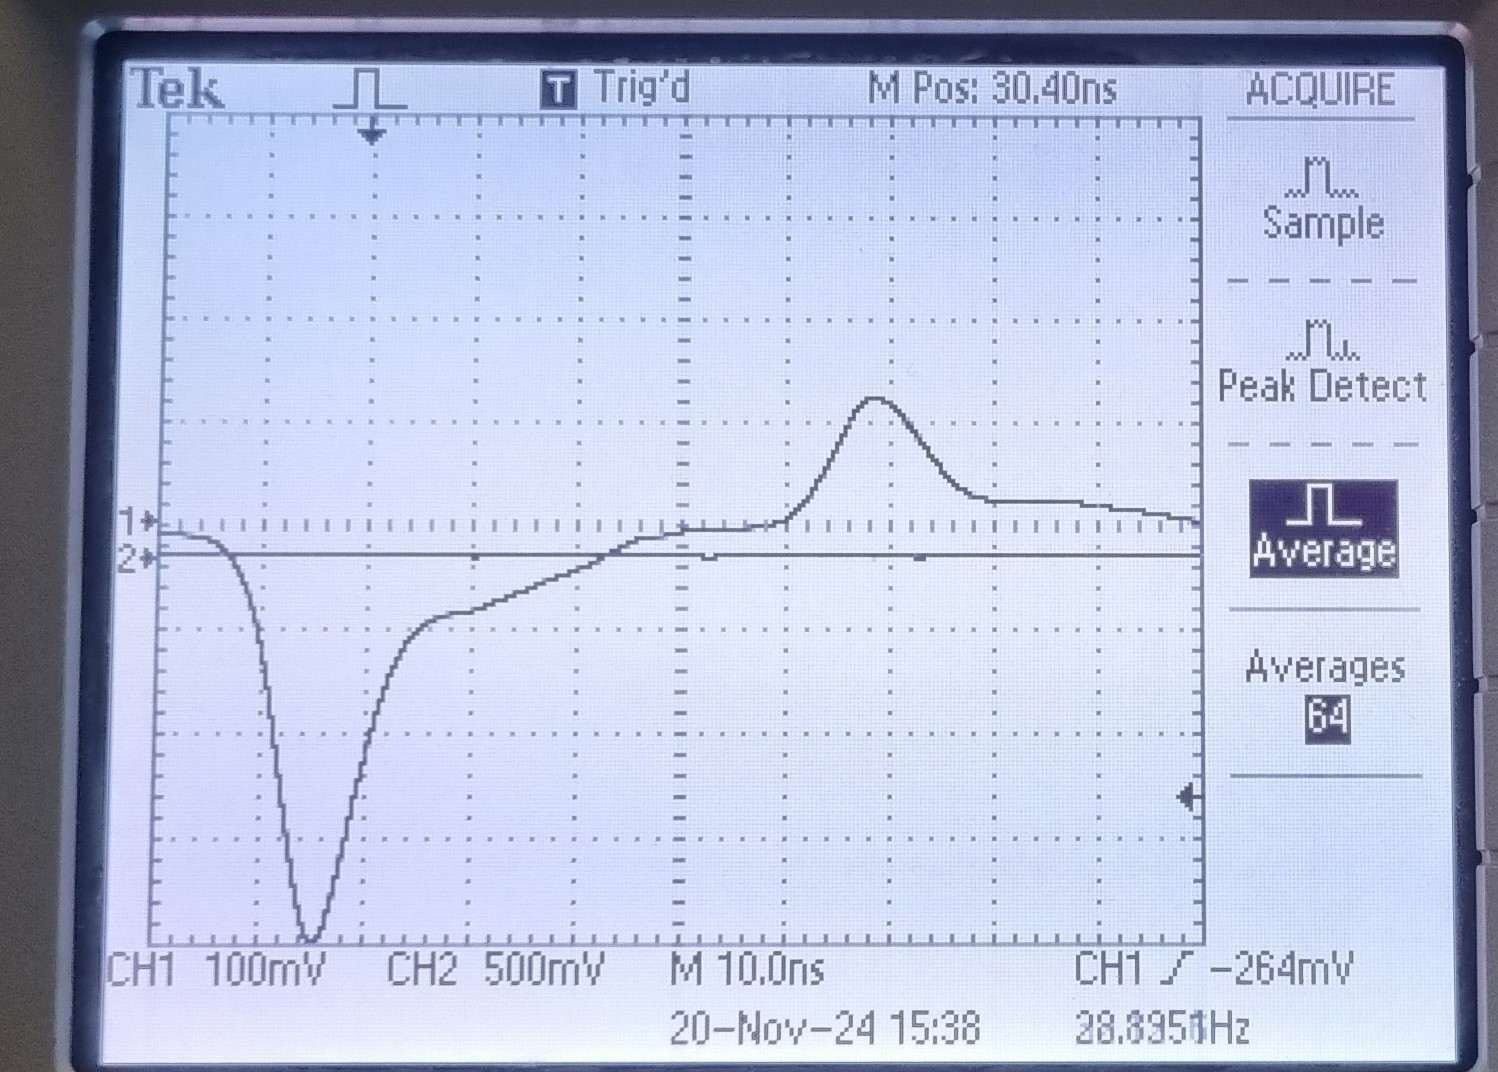
\includegraphics[height=0.33\linewidth]{pmt_cfd_signals/pmt3.jpg}
    \quad
    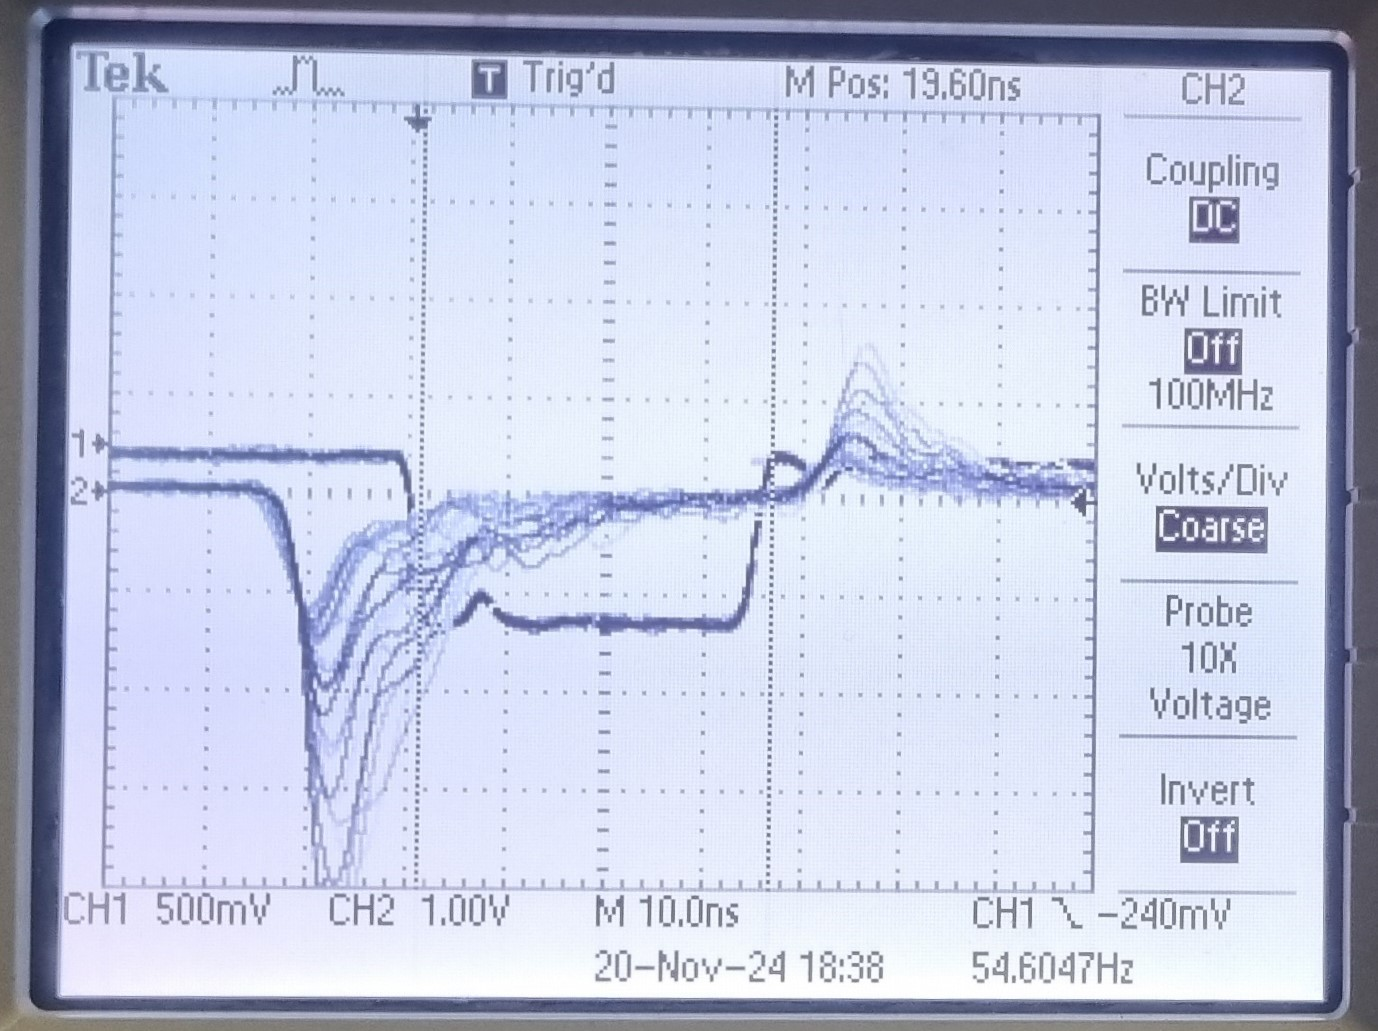
\includegraphics[height=0.33\linewidth]{pmt_cfd_signals/cfd.jpg}
    \caption{Average anode signal from the $\mathtt{UP_{left}}$ PMT (on the left) and signals from the same PMT triggered by the corresponding discriminator signals (on the right).\protect\footnotemark}
    \label{fig:pmt signals}
\end{figure}
\footnotetext{In the picture on the right, the vertical scale of Ch2 of the oscilloscope is amplified by a factor 10.} 

In Tab. \ref{tab:pmt_signals} the significative values for the description of this average signal are reported for $\mathtt{UP_{left}}$ and $\mathtt{UP_{right}}$; these measurements were done with the cursors of the oscilloscope by using the average mode set on $64$ (as shown in Fig. \ref{fig:pmt signals}). 
The $\mathrm{DOWN}$ signals, instead, were observed but not directly measured, that's the reason why they are not reported in Tab. \ref{tab:pmt_signals}.  
Let us point out that $t_{\mathrm{rise}}$ was calculated considering all the peaks of the signal (i.e. the time of rise was considered to be the time required to the signal to go back to the noise level), whereas $V_{\mathrm{max}}$ was evaluated just looking at the first (negative) peak.\footnote{The uncertainties on the oscilloscope were estimated using the formulas on the manual \url{https://download.tek.com/manual/071181702web.pdf}.}

\begin{table}[H] 
    \centering
    \captionsetup{width=.8\linewidth}
    \begin{tabular}{|l|cccc|}
         \hline
         & $t_{\mathrm{fall}}\, \mathrm{(ns)}$ & $t_{\mathrm{rise}}\, \mathrm{(ns)}$ & $V_{\mathrm{max}}\, \mathrm{(mV)} $ & $V_{\mathrm{noise}}\, \mathrm{(mV)}$\\
         \hline
         UP LEFT &  $7.6\pm0.4$& $175\pm1$ & $544\pm9$  & $\approx 2.0$\\ %Vnoise to 8ns
         UP RIGHT & $13.4\pm0.2$& $169\pm1$ & $328\pm5$  & $\approx 1.2$\\
        % DOWN LEFT &  $\simeq 10\, \mathrm{ns}$ & & $\simeq1100$ & & \\
         %DOWN RIGHT &   \\
         \hline         
    \end{tabular}
    \caption{Falling time, rising time, negative peak height of the average anode signals and noise level estimation from the $\mathtt{UP_{left}}$ and $\mathtt{UP_{right}}$ PMTs} 
    \label{tab:pmt_signals}
\end{table}

Each PMT anode signal was connected to the input of a leading edge discriminator. For a given PMT output, the discriminator threshold value should be set so that the rate of high enough events is compatible with the expected rate of muon events, which is $\approx\!40$ Hz. However, a lower threshold value is preferable in order to not miss muon signals that are attenuated by propagation of light inside the scintillator. The value was chosen so as to have a counting rate of about 70 Hz, which was measured by means of a CAEN scaler with a preset timer of $1\,\mathrm{s}$. By observing the anode signals triggered on the discriminator output, it was possible to see that the chosen threshold value is $\approx\!100$ mV. Fig. \ref{fig:pmt signals} on the right gives an example of the threshold that implies a rate of $\approx\!40$ Hz.

%description of scalers

%some photons may be included by setting the threshold higher, but they will be eliminiting by coincidence condition. %not sure if we have to eliminate them with conditions on the histograms

\subsubsection{Coincidences} 
\hypertarget{2.1.2}{}
\paragraph{1. Left and right} Besides threshold setting, a further way to select a muon event in a scintillator is to require that the event is seen by both the left detector and the right detector. 
To do so, the outputs of the discriminators are sent to two coincidence units, one for each of the following coincidences: 
\begin{center}
$\mathtt{UP_{left}\wedge UP_{right}^\mathrm{(delayed)}\equiv UP}$ $~~~~~~~~~~~~~\mathtt{DOWN_{left}\wedge DOWN_{right}^\mathrm{(delayed)}\equiv DOWN}$ %$\mathtt{T_1\vee T_2\equiv T}$ %Here $\mathtt{T_1}$     
\end{center}
For a given scintillator, the right signal is delayed of a time $D_1$ before being sent to the coincidence unit: in this way, the timing information of the output of the coincidence unit corresponds to the right signal one. 
The widths of the discriminators’ signals and the delays $D_1$ (Tab. \ref{tab:coincidences}) have the effect shown in Fig. \ref{fig:coincidences}: it may be seen that, for both scintillators, timing overlap is guaranteed and always starts with the right signal. 
The overlapped output signal can be seen in Fig. \ref{fig:overlapped}. %\footnote{Here again the vertical scale of Ch.2 of the oscilloscope is amplified by a factor 10.} 
The time distance between the two NIM signals in those panels, whose values are shown in Tab. \ref{tab:coincidences}, is equal to $D_1+D_2$, where $D_2$ is the characteristic I/O delay time of the circuit. It may be seen that $D_2\approx15$ ns.

The counting rates of left-right coincidence events turn out to be lower than 70 Hz.
% Table \ref{tab:coincidences} also shows the counting rates of left-right coincidence events in the two scintillators, measured by means of the CAEN scaler.
% 
% \begin{multicols}{2}
% \begin{itemize}
%     \item Coincidence 
%     $\mathtt{UP_{left}\wedge UP_{right}\equiv UP}$;
%     \item Coincidence $\mathtt{DOWN_{left}\wedge DOWN_{right}\equiv DOWN}$;
%     \item Coincidence $\mathtt{UP\wedge DOWN}$;
%     \item Coincidence $\mathtt{UP\wedge DOWN\wedge T}$, with $\mathtt{T=T_1\vee T_2}$.
% \end{itemize}
% \end{multicols}

\begin{table}[H]
    \centering
   % \captionsetup{width=.9\linewidth}
    \begin{tabular}{|l|cccc|}
    \hline
        Coincidence & \multicolumn{2}{c}{width (ns)} & $D_1$ (ns)& $D_1+D_2$ (ns)\\
        &$\mathtt{left}$&$\mathtt{right}$&&\\
        \hline
        
        $\mathtt{UP}$ & $44.8\pm0.7$ & $44.9\pm0.7$ & $\approx26$ &$\approx42$\\
        $\mathtt{DOWN}$ & $47.6\pm0.7$ & $46.6\pm0.7$ & $\approx24$ & $\approx38$\\
        \hline
    \end{tabular}
    \caption{Widths of left and right discriminator signals, delay $D_1$ of the right signal and total delay $D_1+D_2$ of the overlapped output with respect to the left signal, for coincidence $\mathtt{UP}$ and coincidence $\mathtt{DOWN}$}
    \label{tab:coincidences}
\end{table}

\begin{figure}[H]
    \centering
   % \captionsetup{width=.92\linewidth}
    \subfloat[][$\mathtt{UP}$]
    {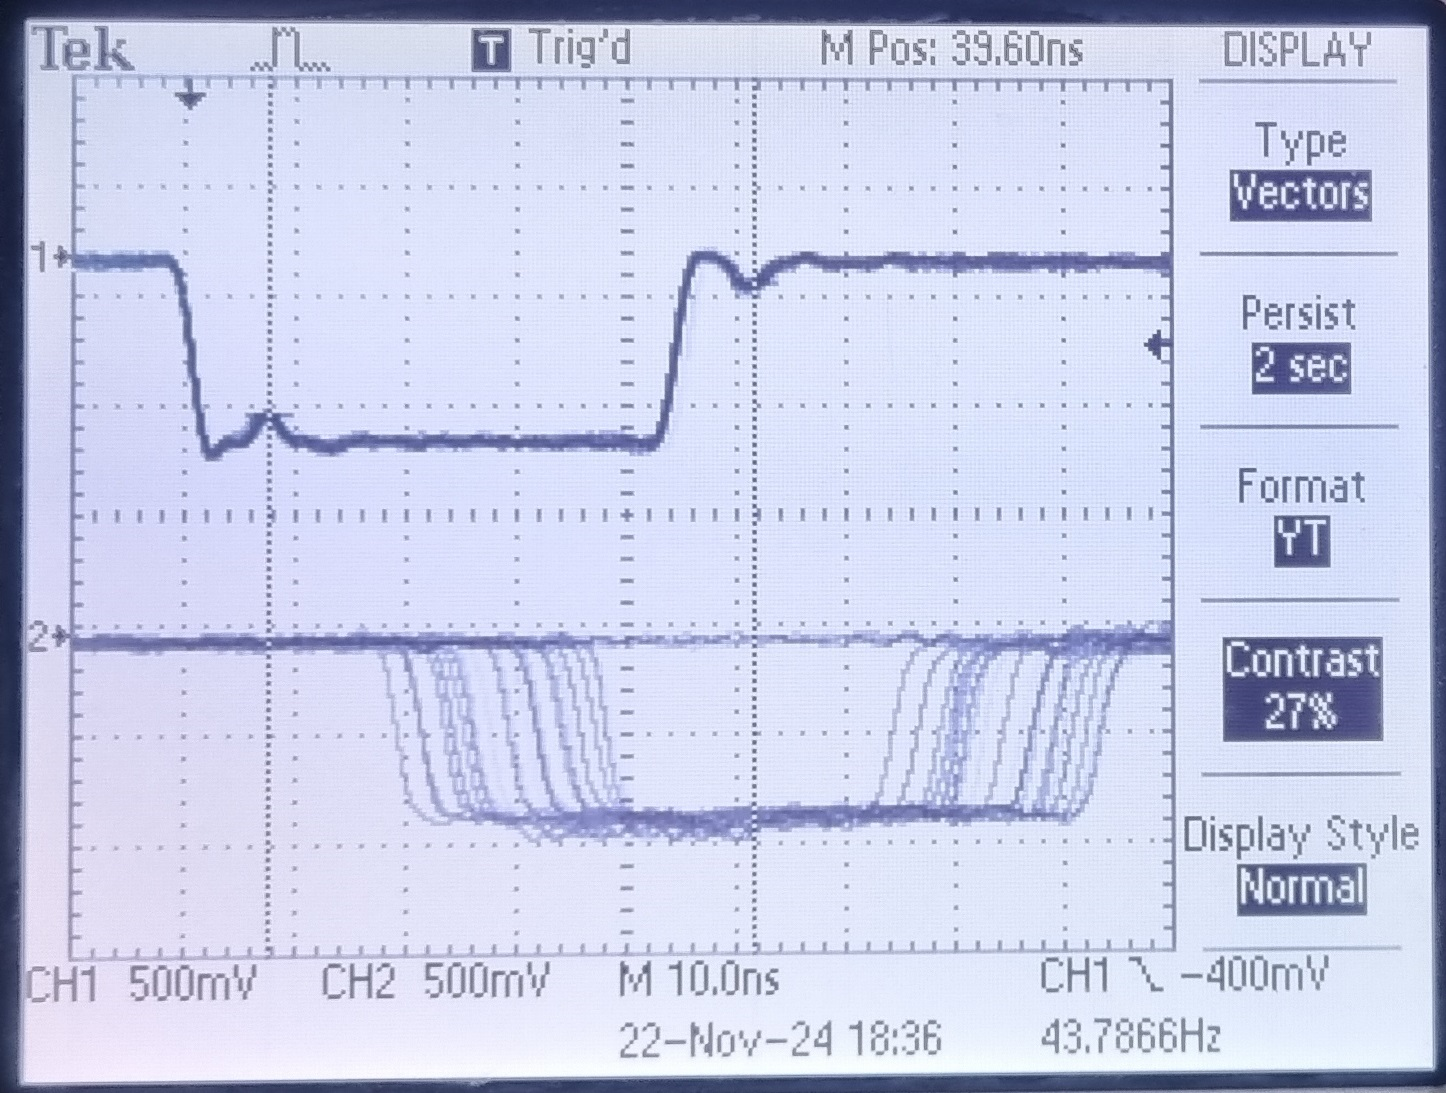
\includegraphics[height=0.35\linewidth]{Figures_Coincidences/C1_Up.jpg}}\quad\quad\quad
     \subfloat[][$\mathtt{DOWN}$]
     {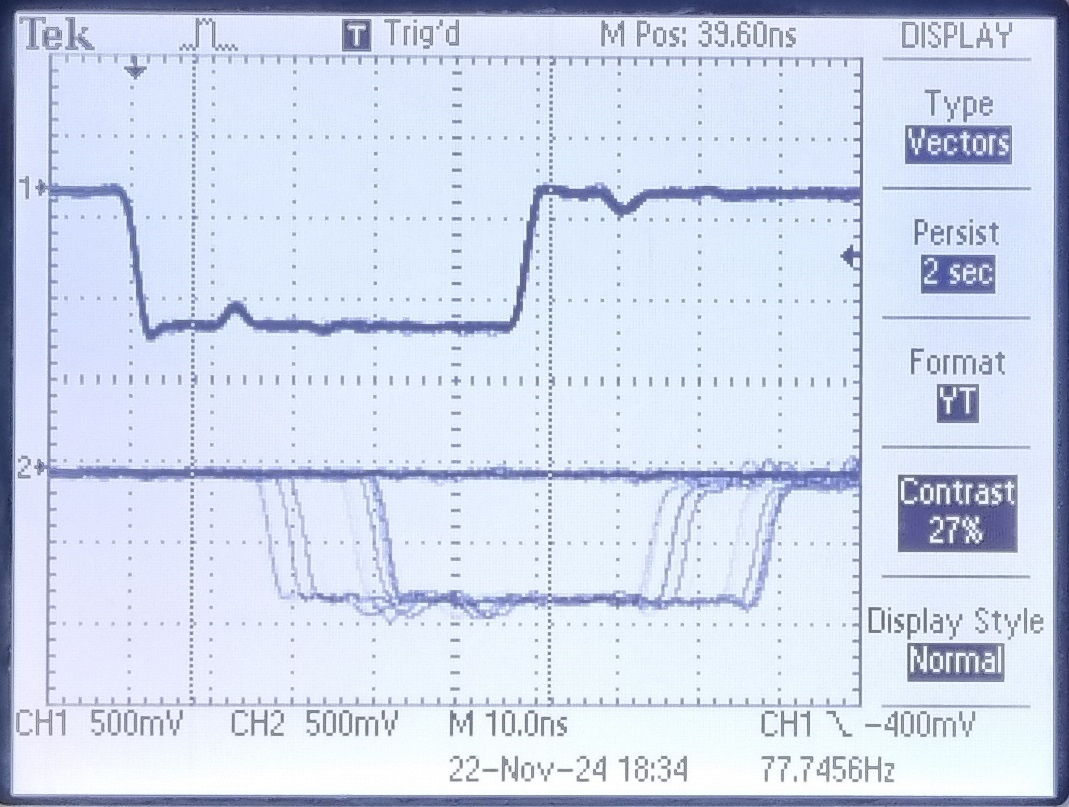
\includegraphics[height=0.35\linewidth]{Figures_Coincidences/C2_Down.jpg}}\quad
     % \subfloat[][$\mathtt{UP Left and Right}$]  {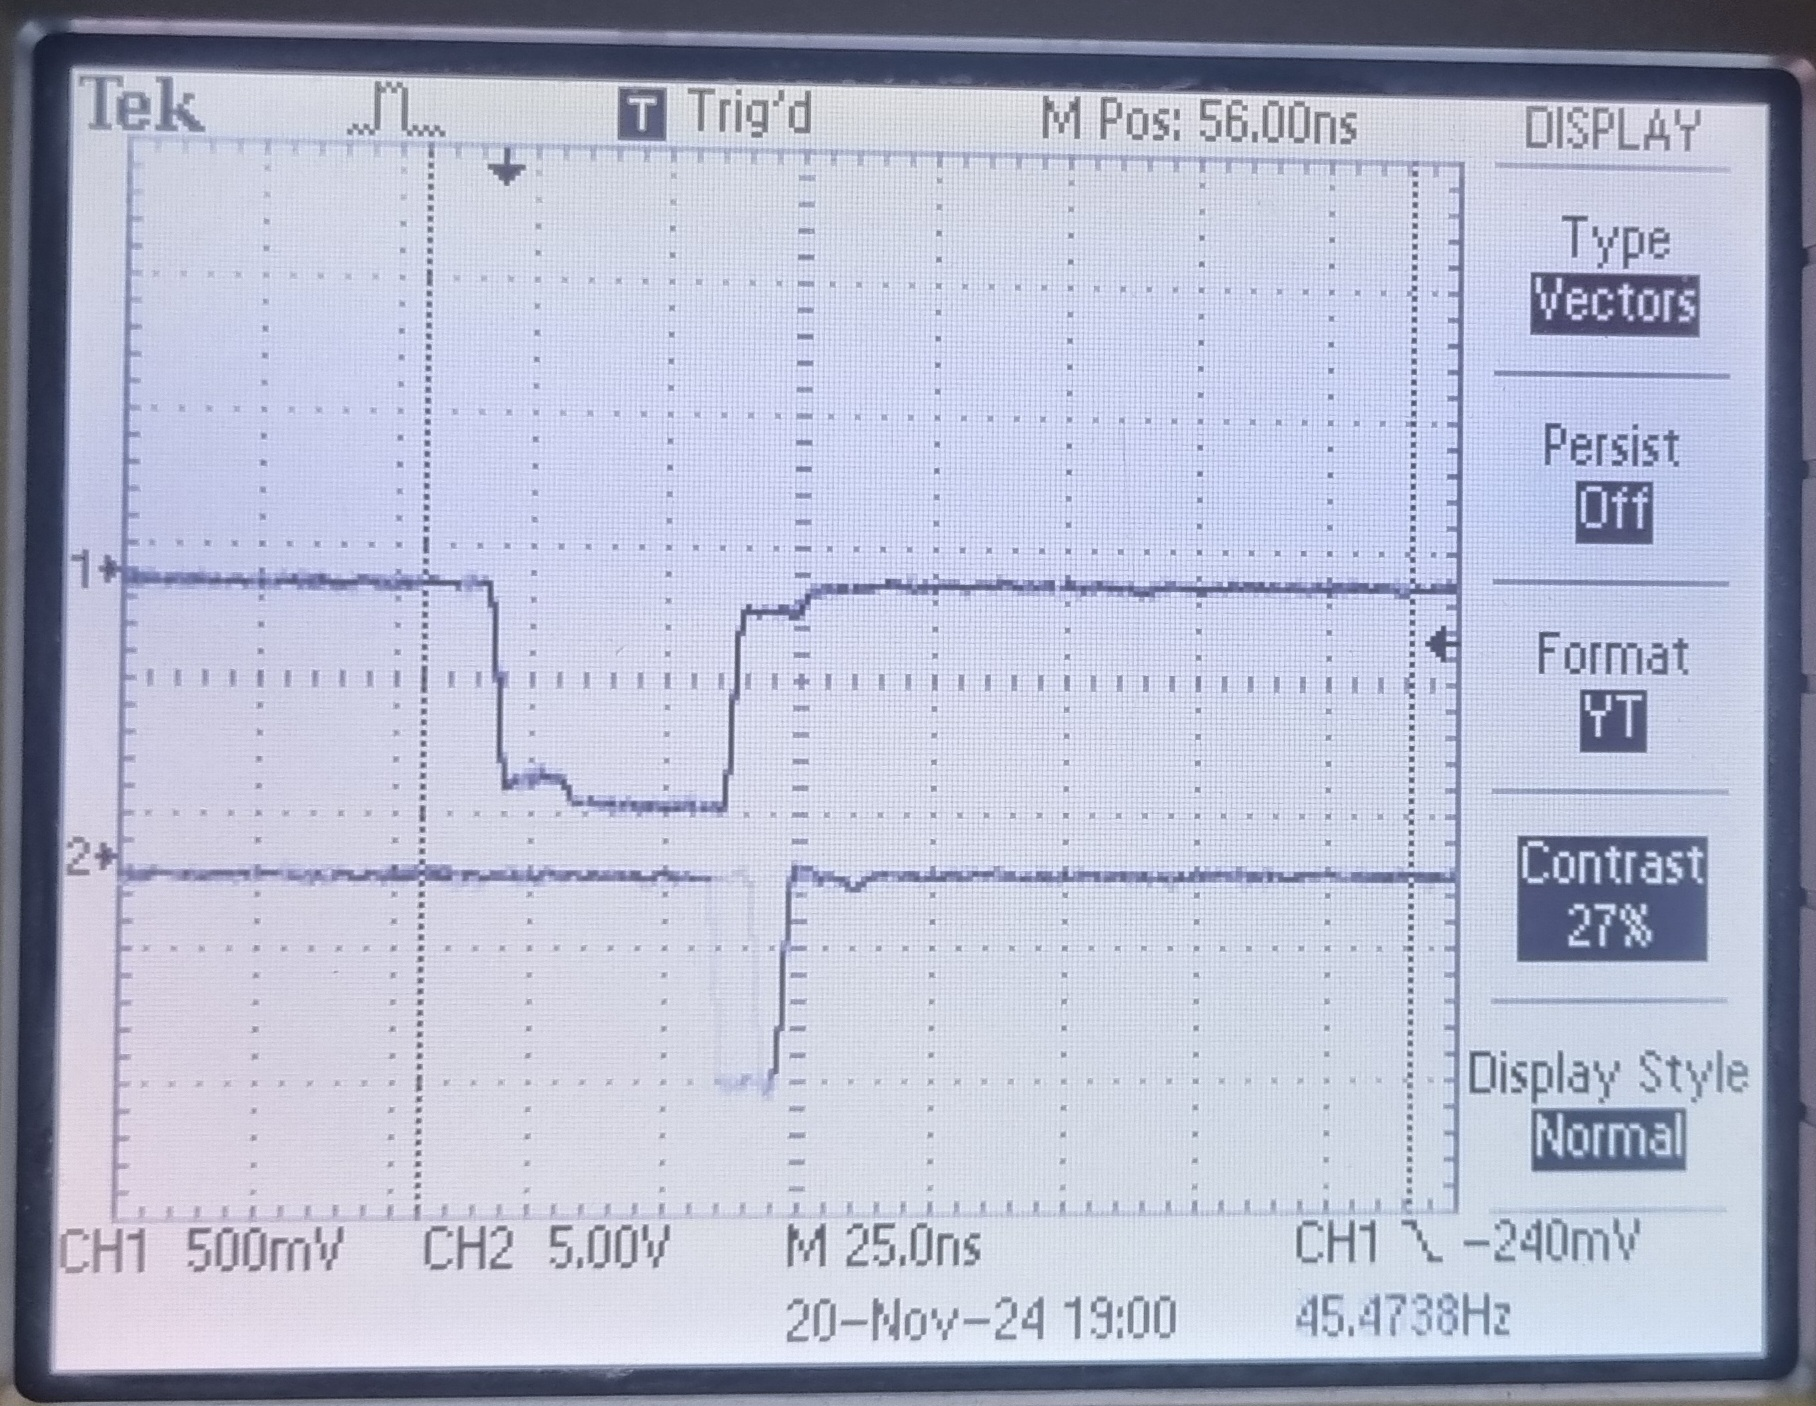
\includegraphics[width=0.3\textwidth]{Figures_Coincidences/C5_left-and-right.jpg}}
    %  \subfloat[][]
    %  {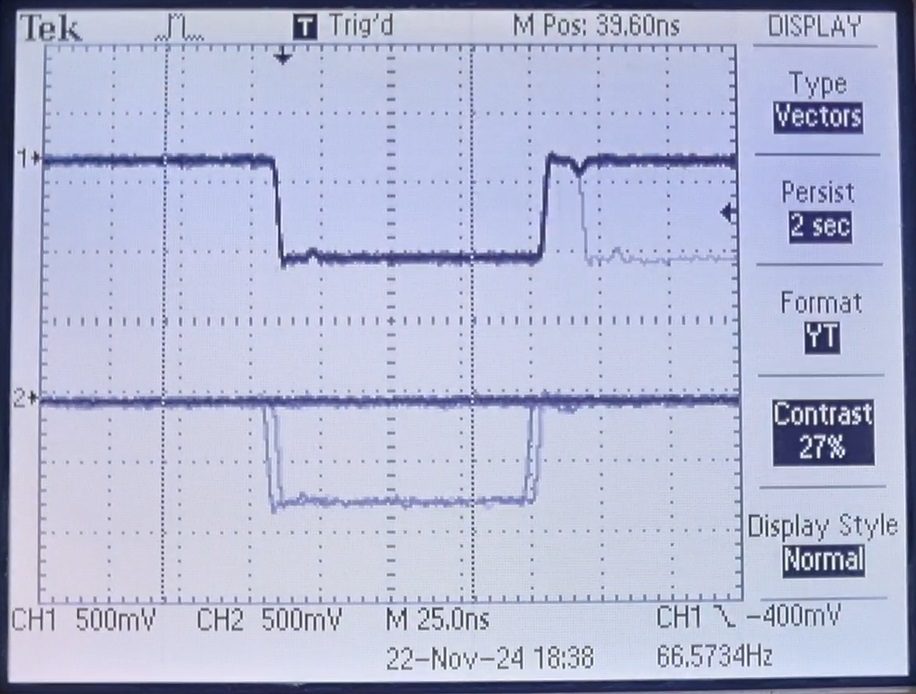
\includegraphics[width=0.35\textwidth]{Figures_Coincidences/C3_Up-and-down.jpg}}\quad\quad\quad
    % \subfloat[][]
    %  {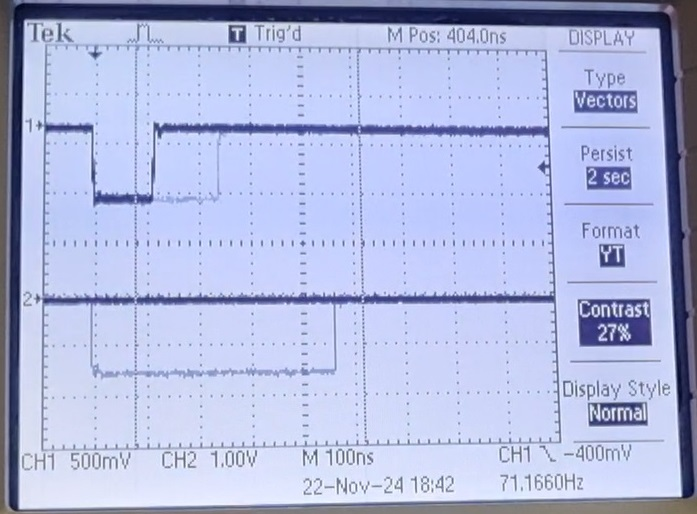
\includegraphics[width=0.35\textwidth]{Figures_Coincidences/C4_Up & down & T.jpg}}
     \caption{Inputs of left-right coincidence units: \textbf{(a)} scintillator UP, \textbf{(b)} scintillator DOWN. In every panel, Ch1 is the left signal while Ch2 the right one.%; in the last panel, Ch1 is  \textcolor{red}{can we add this?}
     }
     %Ch1 $\mathtt{UP_{left}}$, Ch2 $\mathtt{UP_{right}}$ delayed; \textbf{(b)} Ch1 $\mathtt{DOWN_{left}}$, Ch2 $\mathtt{DOWN_{right}}$ delayed.; \textbf{(c)} Ch1 $\mathtt{UP}$, Ch2 $\mathtt{DOWN}$; \textbf{(d)} Ch1 $\mathtt{UP\wedge DOWN}$, Ch2 $\mathtt{T}$ \textcolor{blue}{[This figure is just an idea (it could also have a better appearance)]}}
    \label{fig:coincidences}
\end{figure}
\vspace{-0.5 cm}
\begin{figure}[H]
    \centering
  %  \captionsetup{width=.9\linewidth}
     \subfloat[][$\mathtt{UP}$]
     {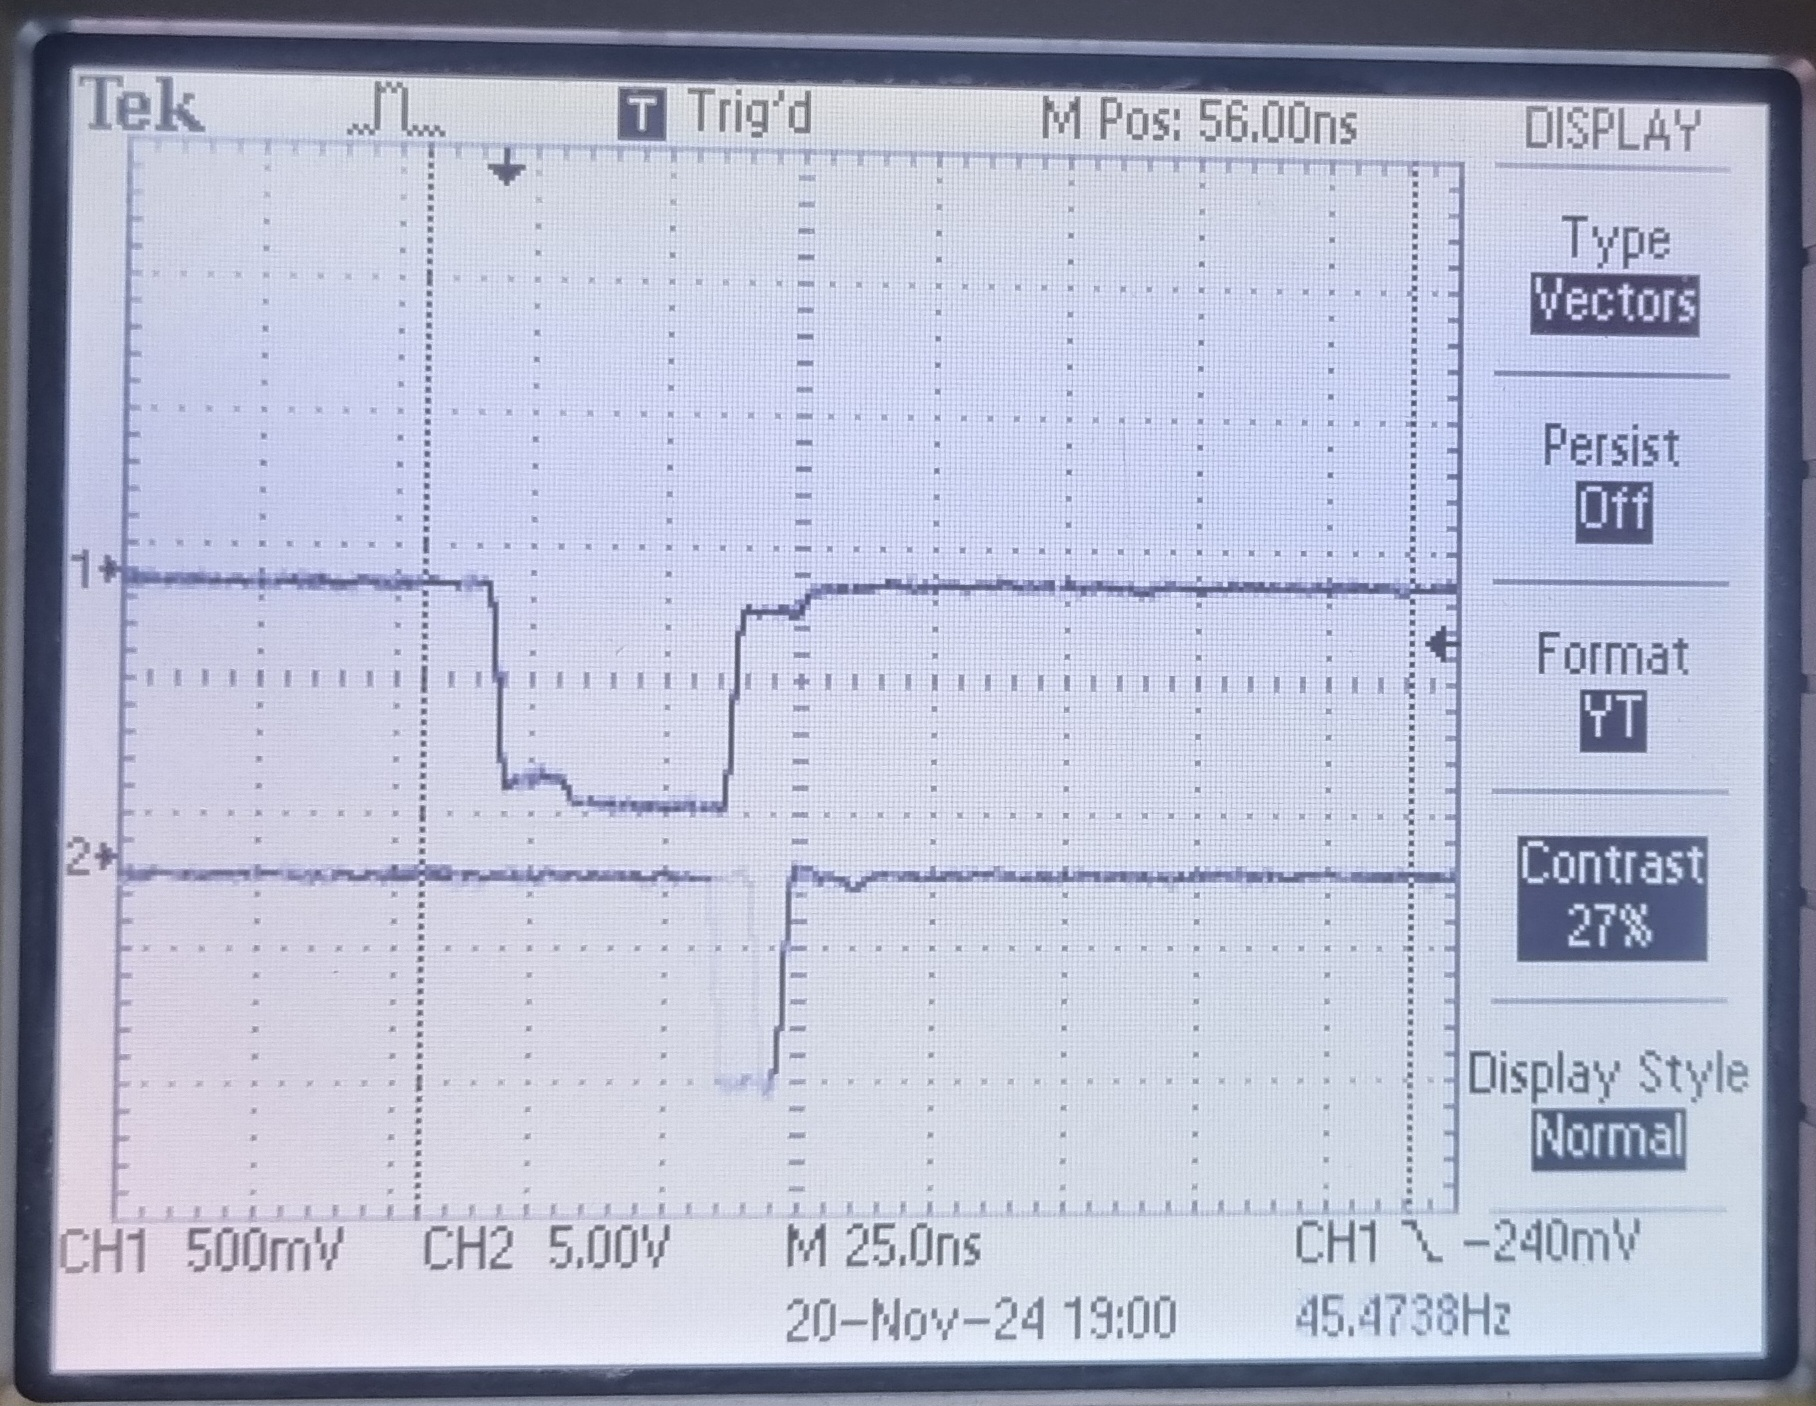
\includegraphics[height=0.35\linewidth]{Figures_Coincidences/C5_left-and-right.jpg}}\quad\quad\quad
     \subfloat[][$\mathtt{DOWN}$]
     {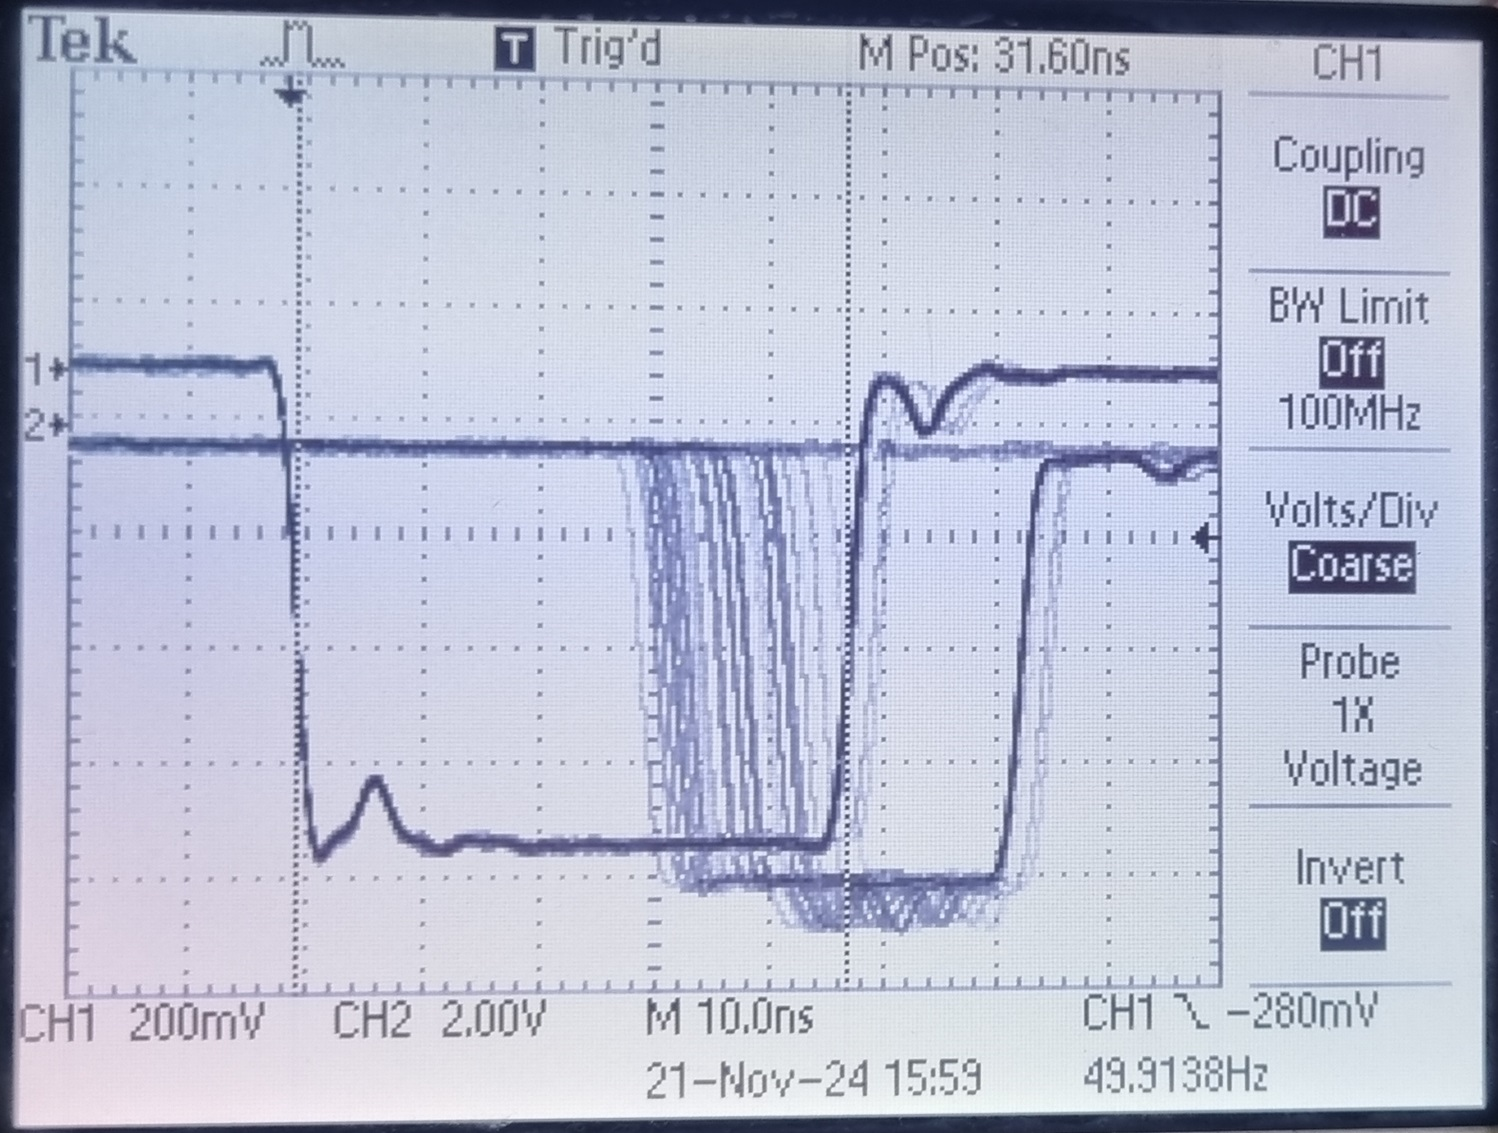
\includegraphics[height=0.35\linewidth]{Figures_Coincidences/overlapped_down.jpg}}
     \caption{Overlapped output signal from coincidence units \textbf{(a)} $\mathtt{UP}$ and \textbf{(b)} $\mathtt{DOWN}$. In every panel Ch1 is the left signal, while Ch2 is the overlapped output signal\protect\footnotemark.}
    \label{fig:overlapped}
\end{figure}
\footnotetext{Here again the vertical scale of Ch2 of the oscilloscope is amplified by a factor 10.}

\paragraph{2. Up and down}The output of the previous coincidence units are used as the inputs of another coincidence unit, which realizes the coincidence  $\mathtt{UP\wedge DOWN}$. 
Its output in turn is used as the trigger for the DAQ, thus limiting the directions of the accepted muons. 

The measured rate of these signals was calculated by recording the TAC scaler counts of the events arriving in $1\,\mathrm{s}$ during a time of $\approx20\,\mathrm{s}$ and then calculating their mean. The obtained value is $(3.0\pm0.4)\,\mathrm{Hz}$, where the uncertainty estimation is the standard deviation of the mean. 
% \textcolor{blue}{$(3%47619
% \pm2)$ Hz, where the uncertainty estimation is \textit{the square root of the mean value, according to the Poisson distribution} OR \textit{the empirical standard deviation}. (same value) OR $(3.5\pm0.4)$ if we consider the standard deviation of the mean} 

\paragraph{3. With the trackers} 
The output of each tracker, after being amplified, is connected to the input of a fast discriminator. 
The following coincidences are made: 
\begin{center}
$\mathtt{T_{1,up}\wedge T_{1,down}\equiv T_1}$ $~~~~~~~\mathtt{T_{2,up}\wedge T_{2,down}\equiv T_2}~~~~~~~$ $\mathtt{T_1\vee T_2\equiv T}$ %Here $\mathtt{T_1}$     
\end{center}
The output of the latter is sent to CH3 of the digitizer. The rate of the coincidence $\mathtt{T}$, measured with the CAEN scaler as explained above, is $(0.5\pm0.2)$ Hz. %OR $(0.5\pm0.6)$ Hz}.
The rate of the coincidence $\mathtt{UP \wedge DOWN \wedge T}$ turns out to be so low that the range of the CAEN scaler, set to $1\,\mathrm{s}$, is not enough to get a measure different from zero.

\subsubsection{TACs and time calibration} \label{sect:time calibration}
%UP TAC:
%start of tac: left and right (up)
%stop of tac: up left signal delayed

%same for down

%UP et down TAC:
%start of tac: up left and right 
%stop of tac: down left and right 

%FOR CALIBRATIONS:
%1. UP: up left and right to the delay box and then to the stop of TAC -> then we have a self-coincidence with a delay set in the delay box
%2. DOWN: same
%3. UP and DOWN: ...

%switch to the or position to have trigger for each valid coincidence in one of two detectors

%testo da rivedere in base al paragrafo sopra 
In this experiment three TACs (\textit{Time to Amplitude Converter}) were used: the first two were associated to the time difference between the left and right signals within UP and DOWN scintillators respectively, whereas the third one was related to the time difference between the two scintillators. The START and STOP signals of each TAC are summarized in the following table (Tab. \ref{tab:TACs}); in the third column the delay $T_d$ of the STOP with respect to the START is mentioned and in the fourth the TAC range is specified. The outputs were connected to the digitizer channels written in the last column. 
In the next pictures (Fig. \ref{fig:tacs}), the START and STOP signals for each TAC are shown as they appeared on the oscilloscope screen.

\begin{table}[H]
    \centering
    \begin{tabular}{|l|ccccc|}
    \hline
        TAC & START & STOP & $T_d$ (ns) & range (ns) & Digitizer ch.\\
        \hline
       UP & %$\mathtt{UP_{left} \wedge UP_{right}}$ 
       $\mathtt{UP}$ & $\mathtt{UP_{left}^{(delayed)}}$ & $\approx\! 20 \, \mathrm{ns}$& $\approx\!50\cdot10/10$& CH1\\
        DOWN & %$\mathtt{DOWN_{left} \wedge DOWN_{right}}$
        $\mathtt{DOWN}$& $\mathtt{DOWN_{left}^{(delayed)}}$ & $\approx \!20 \, \mathrm{ns}$& $\approx\!100\cdot10/10$& CH2\\
       DOWN-UP & $\mathtt{UP}$ %$\mathtt{UP_{left} \wedge UP_{right}}$
       & $\mathtt{DOWN^{(delayed)}}$ %$\mathtt{DOWN_{left} \wedge DOWN_{right}}$
       & $\approx \!20 \, \mathrm{ns}$& $\approx\!100\cdot10/10$& CH0\\
        \hline
    \end{tabular}
    \caption{START and STOP signals on each TAC, delay $T_d$ of the STOP with respect to the START, TAC range and digitizer channel}
    \label{tab:TACs}
\end{table}
    
\begin{figure}[H]
    \centering
    \subfloat[][UP]
    {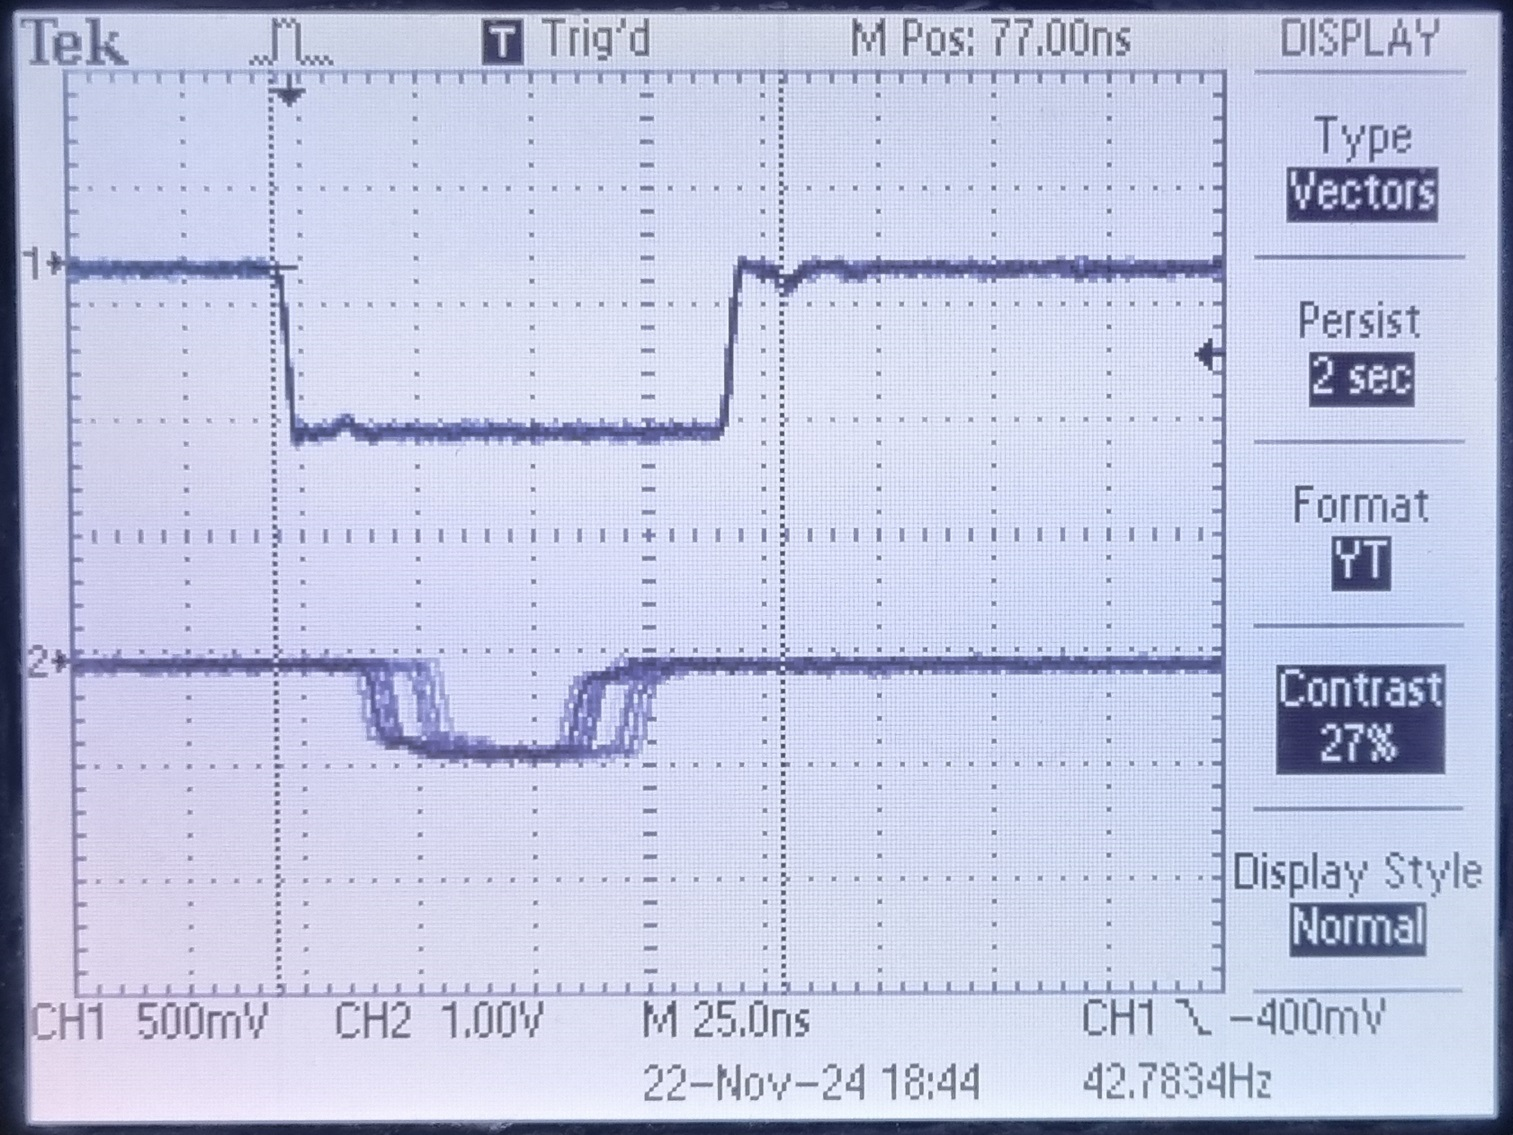
\includegraphics[width=0.30\textwidth]{Figures_TACs/1_TAC up.jpg}}\quad
     \subfloat[][DOWN]
     {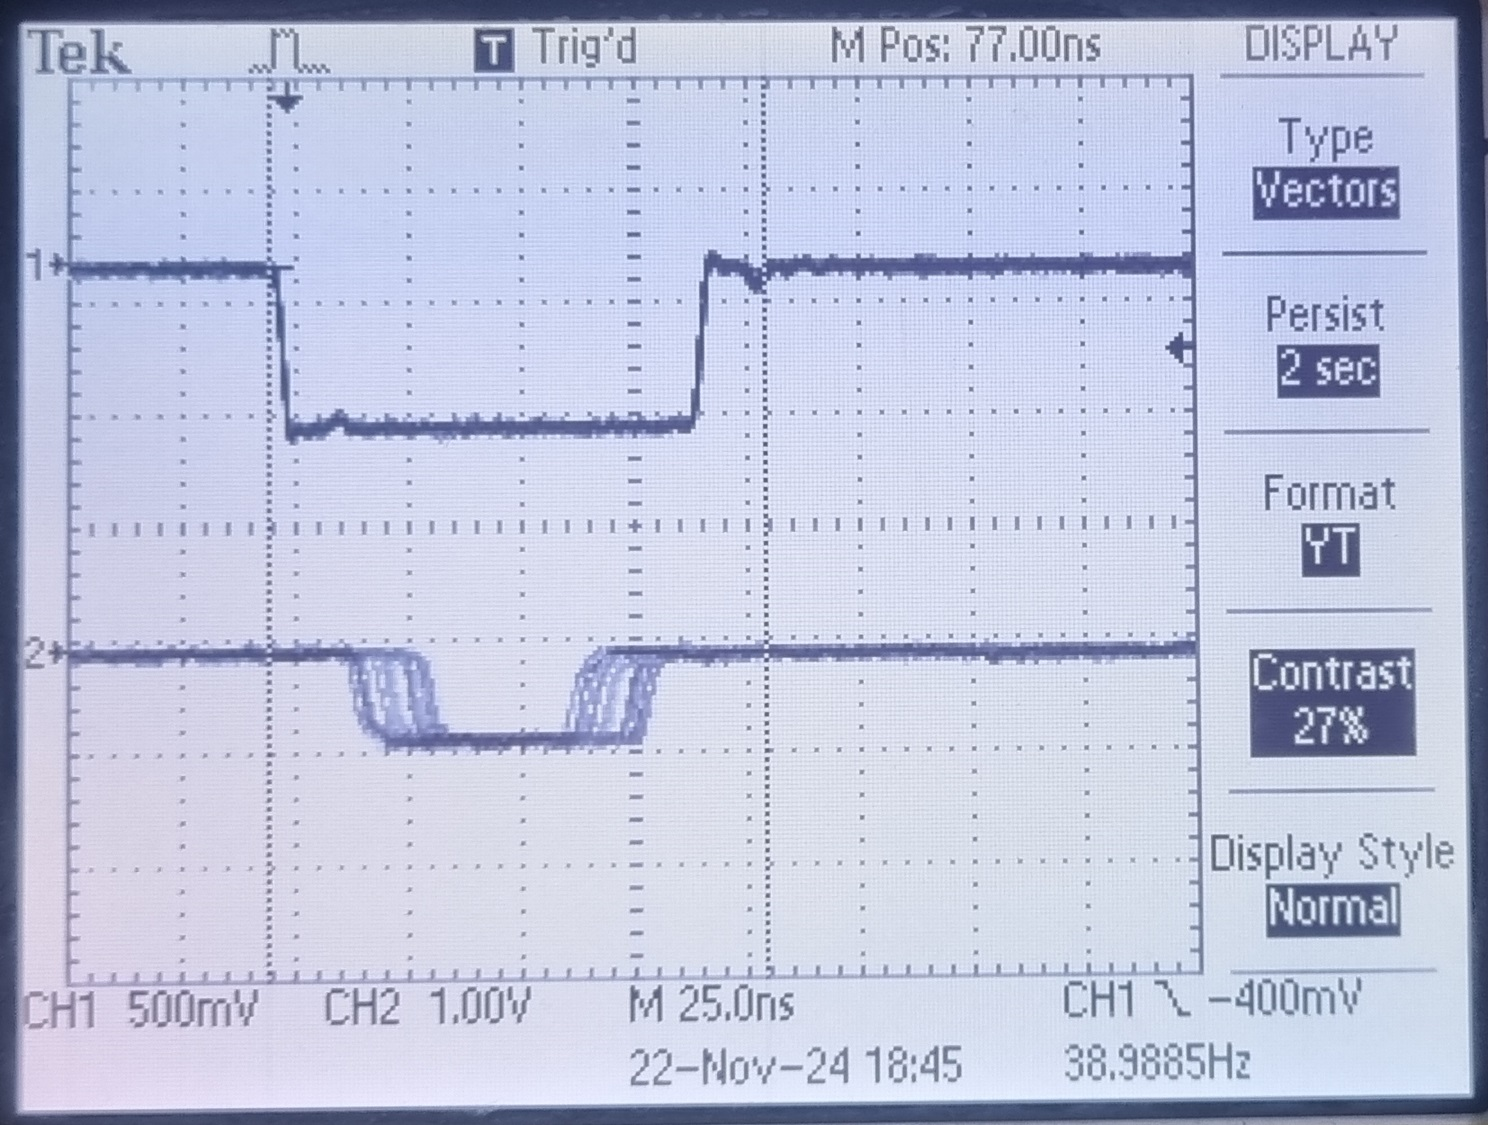
\includegraphics[width=0.30\textwidth]{Figures_TACs/2_TAC down.jpg}}\quad
     \subfloat[][DOWN-UP]
     {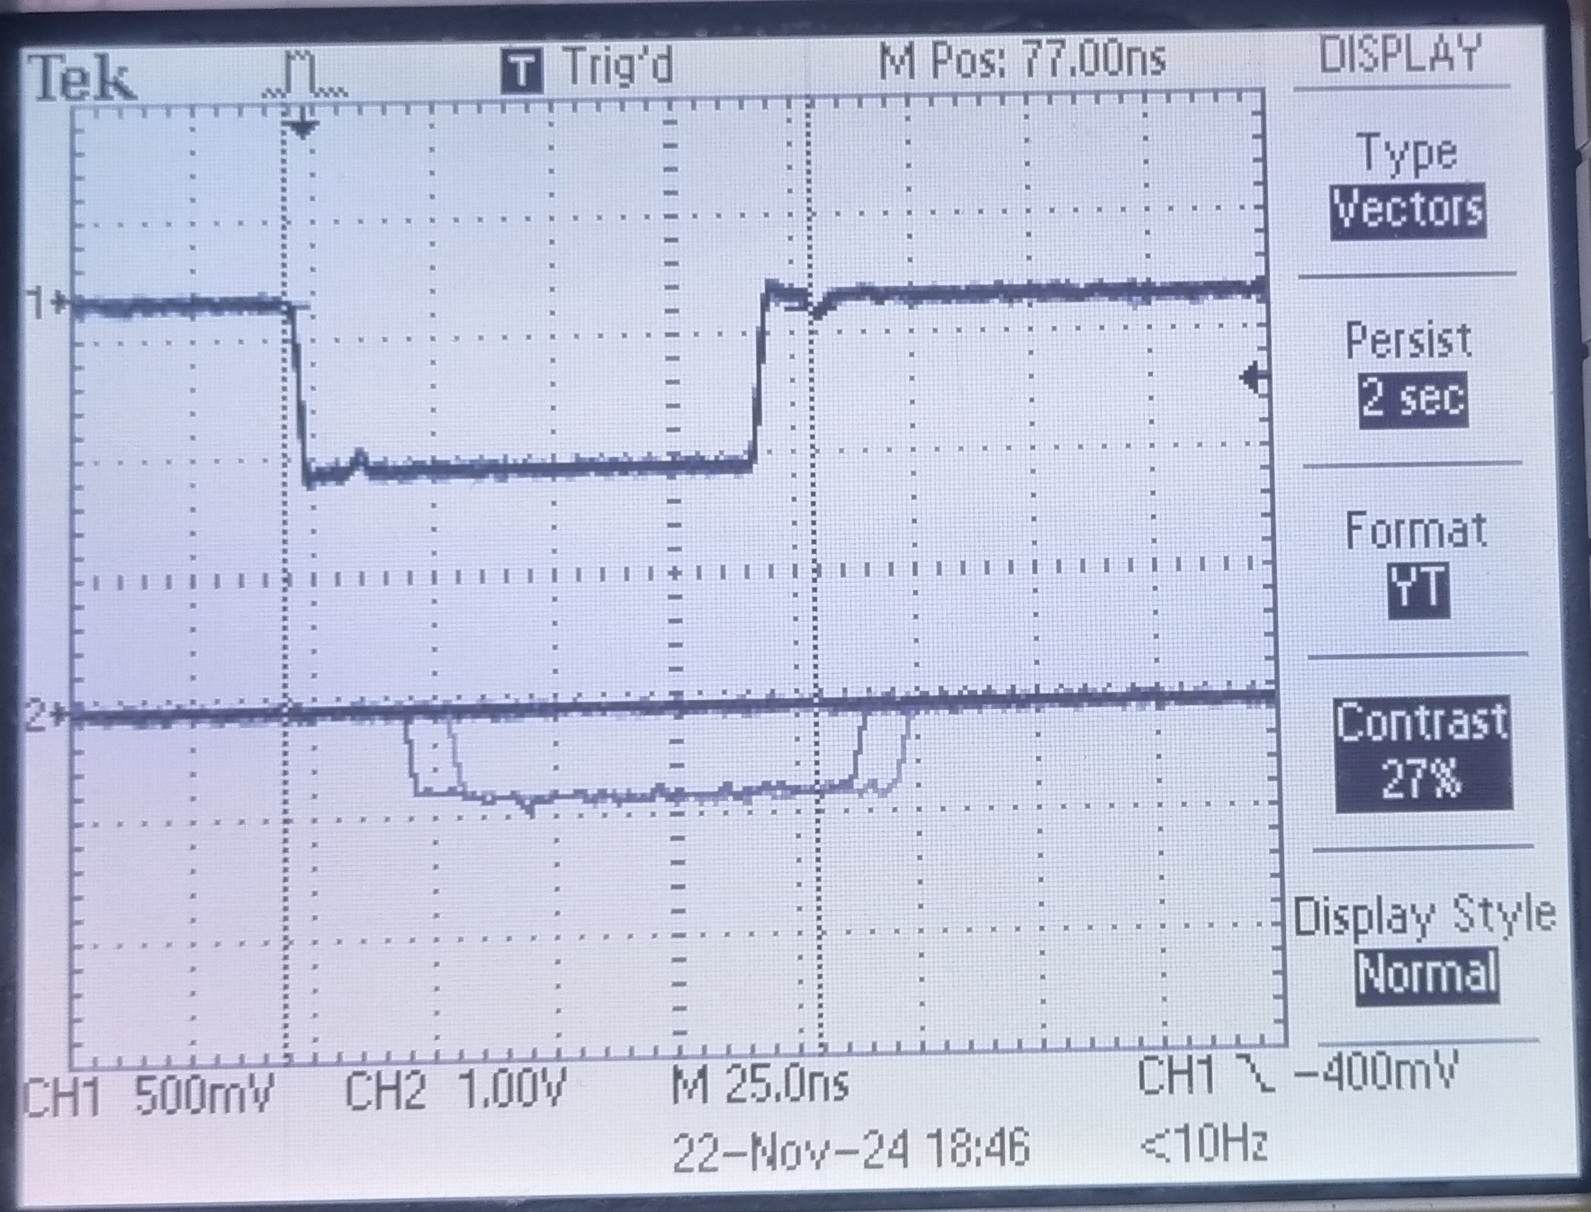
\includegraphics[width=0.30\textwidth]{Figures_TACs/3_TAC up & down.jpg}}
     \caption{Inputs of TACs: \textbf{(a)} UP, \textbf{(b)} DOWN, \textbf{(c)} DOWN-UP. In every panel, Ch1 is the START pulse, while Ch2 is the STOP one.}
    \label{fig:tacs}
\end{figure}

To calibrate the TACs, in time auto-coincidences were made by sending a copy of the coincidence signal -- already connected to the START of the TAC -- to a delay box and then to the STOP of the TAC. Then, by introducing different delays $D$ in the delay box, it was possible to associate the delays in $\mathrm{ns}$ to the ADC channels of the TAC. The trigger signal was $\mathtt{UP\vee DOWN}$. %The delay introduce by the cable is here neglectable.
The same procedure was followed for each TAC. 

For each TAC, the START and STOP signals were observed on the oscilloscope in order to delay enough the STOP signal, which must begin after the START signal. As a consequence, four delays $D$ were chosen and, for every delay, a $\simeq30\,\mathrm{s}$ long data acquisition was done. Then, with a Gaussian fit on the peak, the centroids were determined. The estimate for the delay error is 0.2 ns. %\textcolor{red}{explain the uncertainties on D!} 
The results are shown in the Tab. \ref{tab:tac_cal}.

\begin{table}[H]
    \centering
    \begin{tabular}{|c|ccc|}
    \hline
    $D\,\mathrm{(ns)}$ & $C_{\mathrm{UP}}\,\mathrm{(ch)}$& $C_{\mathrm{DOWN}}\,\mathrm{(ch)}$ & $C_{\mathrm{DOWN-UP}}\,\mathrm{(ch)}$ \\
    \hline
         $26.0\pm0.2$ & $1090.1\pm0.4$& $436.0\pm0.2$& $430.0\pm0.2$\\
         $34.0\pm0.2$ & $1331.0\pm0.6$& $556.4\pm0.3$& $543.8\pm0.2$\\
         $42.0\pm0.2$ & $1569.3\pm0.8$& $675.2\pm0.3$& $655.0\pm0.4$\\
         $50.0\pm0.2$ & $1805.6\pm0.7$& $792.9\pm0.3$& $766\pm1$ \\
    \hline
    \end{tabular}
    \caption{Delays $D$ introduced in the delay box and positions $C$ of the centroids for every TAC}
    \label{tab:tac_cal}
\end{table}

For each set of data in Tab. \ref{tab:tac_cal} a linear fit $C = m\cdot D + q$ was done with delays in $\mathrm{ns}$ and the centroids in ADC channels on the y-axis. The results are shown in the graphics in next picture (Fig. \ref{fig:tac_cal_time}) and in the following table (Tab. \ref{tab:fit_time_cal}). Let us notice from the residual plot that these points fluctuate around zero, as expected from a linear correlation. %fit.

\begin{figure}[H]
    \centering
    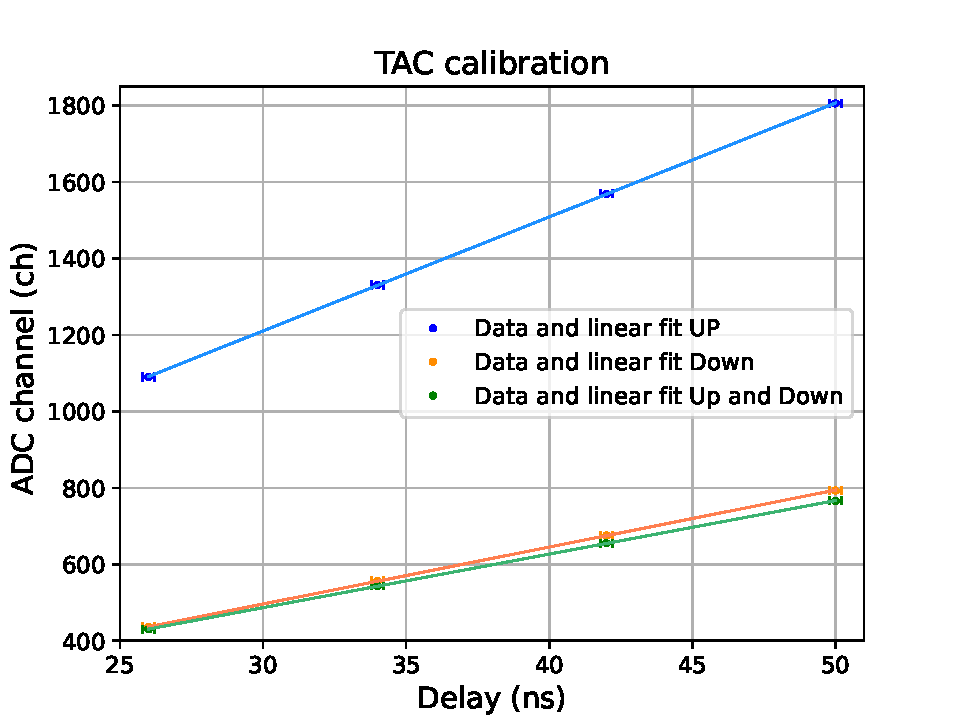
\includegraphics[width=0.48\linewidth]{linear_graph/tac_cal.pdf}
    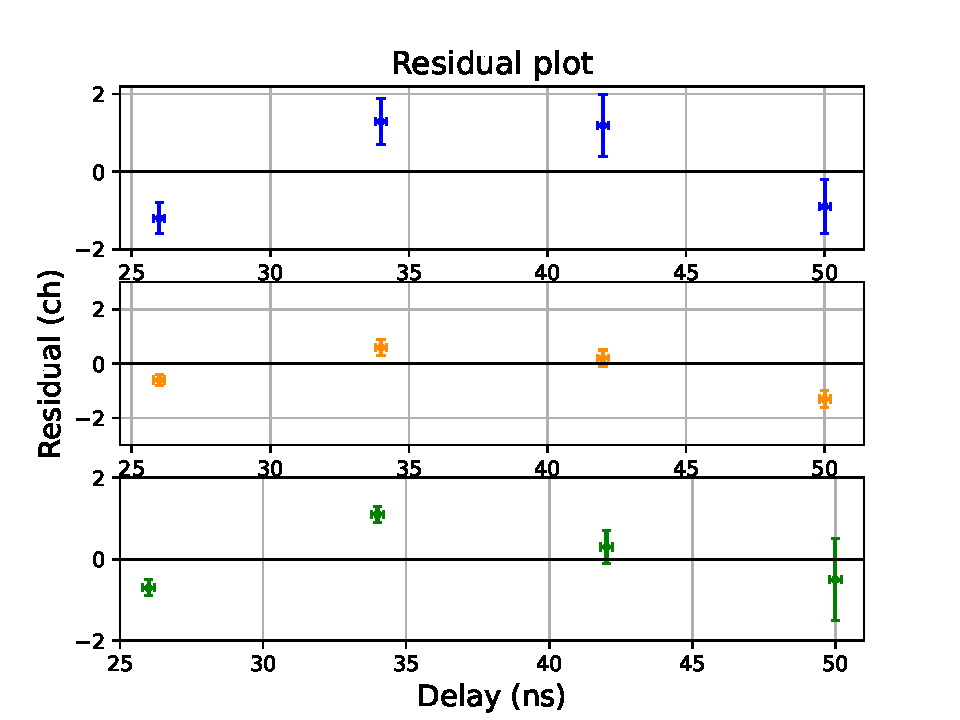
\includegraphics[width=0.48\linewidth]{linear_graph/tac_cal_res.pdf}
    \caption{Calibrations in time for TAC UP (blue), DOWN (orange) and DOWN-UP (green) and residual plot (see Tab. \ref{tab:fit_time_cal})}
    \label{fig:tac_cal_time}
\end{figure}

\begin{table}[H]
    \centering
    \begin{tabular}{|c|c|c|}
         \hline
         $m_{\mathrm{UP}}=(29.8\pm0.3) \, \frac{\mathrm{ch}}{\mathrm{ns}}$ &$m_{\mathrm{DOWN}}=(14.9\pm0.2) \, \frac{\mathrm{ch}}{\mathrm{ns}}$ & $m_{\mathrm{DOWN-UP}}=(14.0\pm0.2) \, \frac{\mathrm{ch}}{\mathrm{ns}}$\\
         $q_{\mathrm{UP}}=(320\pm10) \,\mathrm{ch}$&$q_{\mathrm{DOWN}}=(50\pm7) \,\mathrm{ch}$ & $q_{\mathrm{DOWN-UP}}=(67\pm6) \,\mathrm{ch}$\\
         \hline
         \end{tabular}
    \caption{Results of TACs calibrations in time}
    \label{tab:fit_time_cal}
\end{table}

%By these results it's now possible to obtain the value in $\mathrm{ns}$ for every measure in channels.

\subsection{Observation of the cosmic rays}
After the time calibration, the STOP inputs of the TACs were restored in the original configuration. 
A sample of cosmic rays events was then recorded overnight triggering on the coincidence $\mathtt{UP\wedge DOWN}$. 
Let us remember that CH0, CH1 and CH2 of the digitizer were measuring the quantities described in Tab. \ref{tab:TACs}, while CH3 was connected to the output of the $\mathtt{T}$ coincidence (Sect. \hyperlink{2.1.2}{2.1.2}). %(Sect. \hyperlink{2.1.2}{2.1.2}).

\subsubsection{Calibrated time spectra}
The previous time calibrations of the TAC amplitude spectra (Sect. \ref{sect:time calibration}) allow us to calibrate in time the spectra recorded by the TACs during the overnight acquisition. The resulting histograms are shown in Fig. \ref{fig:tac time spectra}.

\begin{figure}[H]
    \centering
  %  \subfloat[][UP]
    {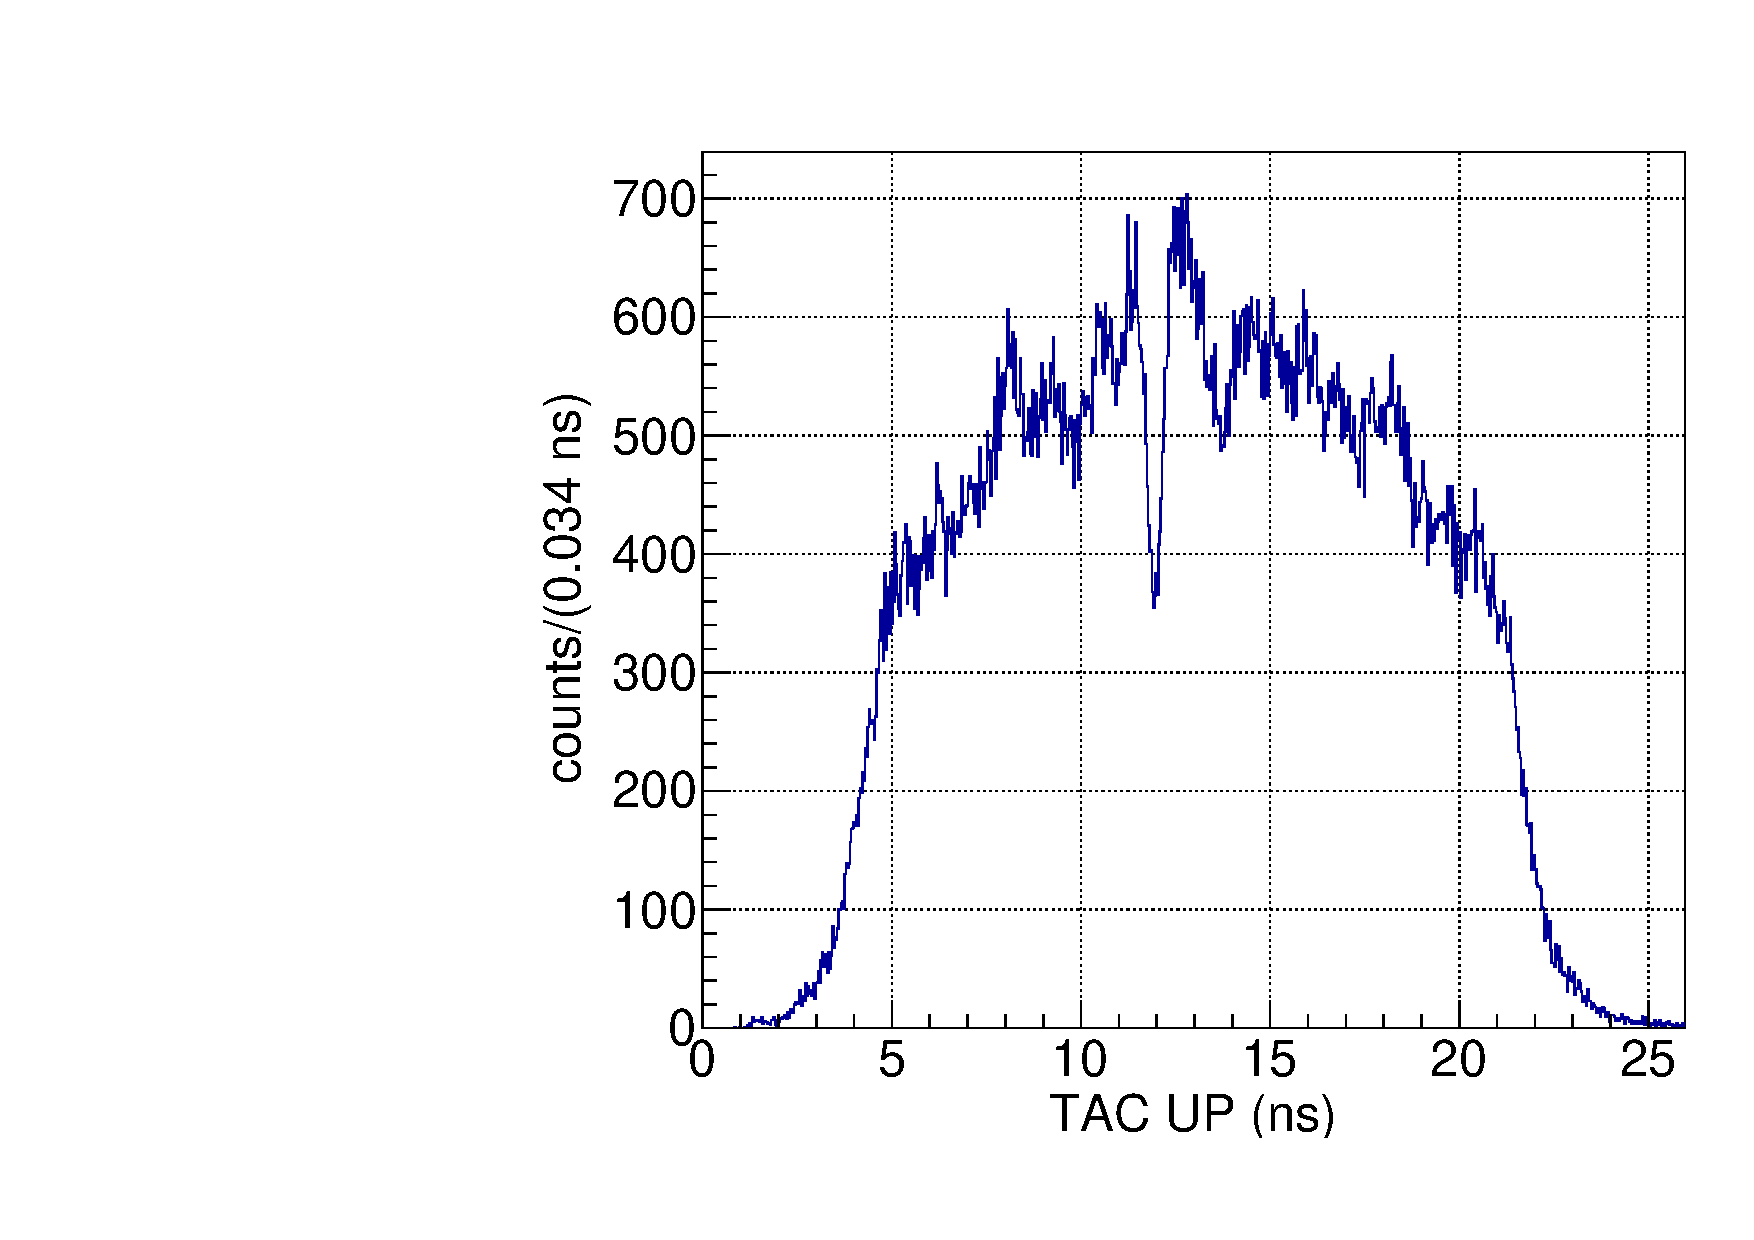
\includegraphics[width=0.32\linewidth]{Figures_TACs/calibrated_UP_3.pdf}}
    % \hspace{-0.1 cm}
   % \subfloat[][DOWN]
    {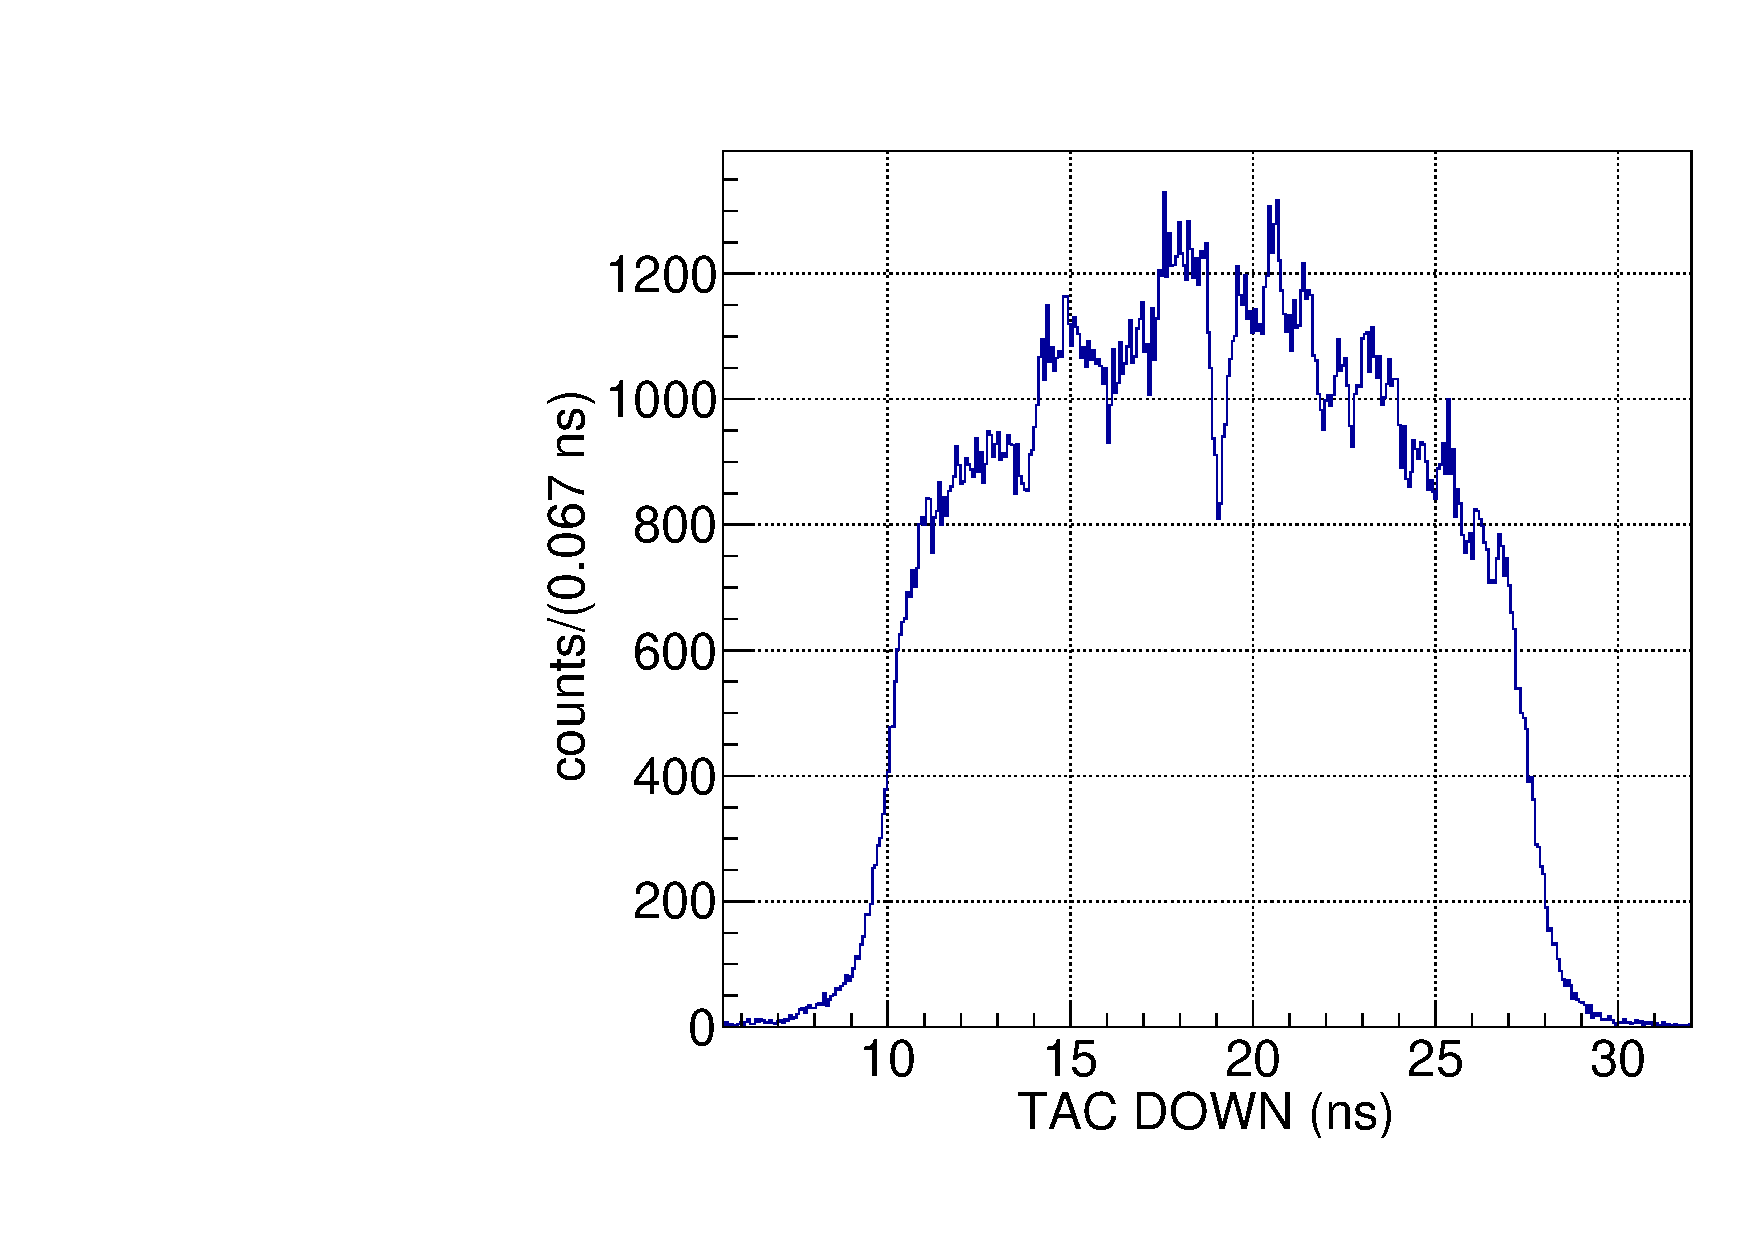
\includegraphics[width=0.32\linewidth]{Figures_TACs/calibrated_down_2.pdf}}
    % \hspace{-0.2 cm}
    % \subfloat[][DOWN-UP]
     {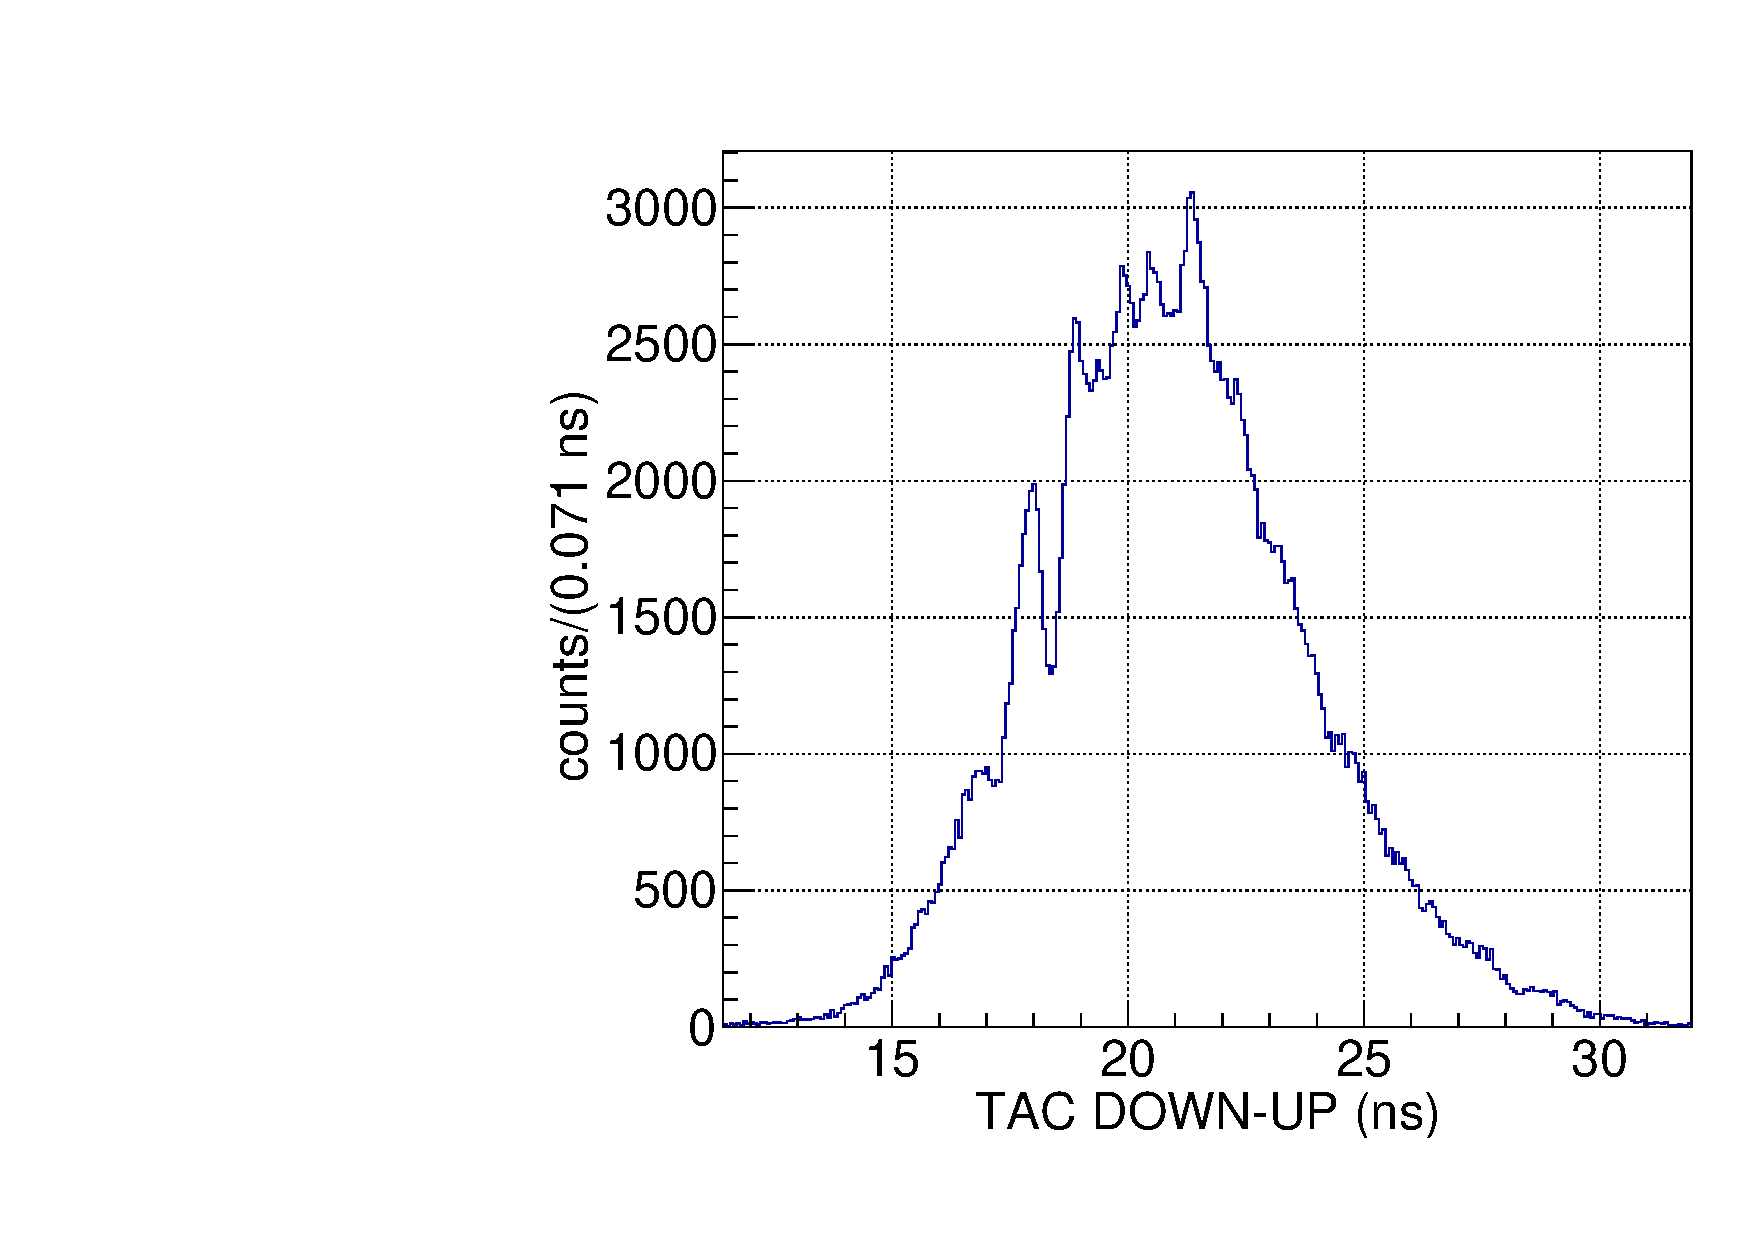
\includegraphics[width=0.32\linewidth]{Figures_TACs/calibrated_downup_3.pdf}}
     % \vspace{0.45 cm}
    %\caption{Time-calibrated spectra from \textbf{(a)} TAC UP, \textbf{(b)} TAC DOWN, \textbf{(c)} TAC DOWN-UP}
    \caption{Time-calibrated spectra from TAC UP, TAC DOWN, TAC DOWN-UP}
    \label{fig:tac time spectra}
\end{figure}

Let us point out that the first two spectra correspond to the distribution of
\begin{equation}\label{eq: time measured by tac up and down}
    \Delta t^{(i)}\equiv t_{\mathrm{left}}^{(i)}-t_\mathrm{right}^{(i)}+T_d^{(i)},\quad\quad i=\mathrm{UP,\,DOWN}
\end{equation}
while the last spectrum measures the distribution of
\begin{equation}\label{eq: time measured by tac down-up}
    \Delta t^{\mathrm{(D-U)}}\equiv t\mathrm{_{right}^{(D)}}-t\mathrm{_{right}^{(U)}}+T_d^\mathrm{(D-U)}
\end{equation}
where $T_d^\mathrm{(U)}$, $T_d^\mathrm{(D)}$, $T_d^\mathrm{(D-U)}\approx20$ ns have been introduced in Tab. \ref{tab:TACs}. Since $t_{\mathrm{left}}^{(i)}-t_\mathrm{right}^{(i)}$ is expected to vary uniformly between $\approx\!-8$ ns and $\approx\!8$ ns, %the first two spectra are expected to be centred at $T_d^{(i)}$. %This is true for TAC DOWN spectrum, whereas TAC UP calibration seems to be affected by a bias. 
the first two spectra are expected to have a width of $\approx \! 16\,\mathrm{ns}$ and to be centred at $T_d^{(i)}$, as indeed\footnote{The UP time spectrum is not centred around $T_d^{(\mathrm{U})}$, so the intercept of the calibration might be slight inaccurate.} obtained for the spectra in Fig. \ref{fig:tac time spectra}.

The first two spectra show a depletion of events almost in the middle of them. Looking at the input signals of the two TACs (Fig. \ref{fig:tacs}a, b), a similar effect may be inferred because the STOP signals appear temporarily split into two groups. Thus, the reason seems not to be a wrong TAC measurement nor a failure of the trigger condition $\mathtt{UP\wedge DOWN}$, but directly a lack of selected events in coincidences $\mathtt{UP_{left}\wedge UP_{right}}$ and $\mathtt{DOWN_{left}\wedge DOWN_{right}}$. 
%(Non so se abbia senso o se vogliamo scriverlo}
 
\subsubsection{Position calibration of TAC UP and TAC DOWN spectra}
The channel spectrum of TAC UP and the one of TAC DOWN plotted in Fig. \ref{fig:position calibration} (upper x-axes) 
%il that era per dire che non sono gli spettri completi
include only the events that produced a signal in CH3, i.e. satisfy the condition $\mathtt{UP\wedge DOWN\wedge T}$. 
Let's estimate the centroids of the peaks, in channels, in Fig. \ref{fig:position calibration}, through Gaussian fits. 
For each spectrum, the centroids are correlated  with the longitudinal positions $x_1\!=\!10$ cm and $x_2\!=\!110$ cm of the trackers with respect to the left end of the scintillators (Tab. \ref{tab:position cal}). Finally, a linear fit was performed for each TAC (Fig. \ref{fig:linear fit for position cal}). 
The obtained position calibrations, shown as the lower x-axis of Fig. \ref{fig:position calibration}, are
\[C_{\mathrm{UP}}=(4.12\pm 0.03)\mathrm{\tfrac{ch}{cm}}\cdot x+(453\pm 2)\,\mathrm{ch} \quad\quad\quad\quad 
C_{\mathrm{DOWN}}=(2.084\pm 0.005)\mathrm{\tfrac{ch}{cm}}\cdot x+(198.9\pm 0.4)\,\mathrm{ch}\]
The position-calibrated spectra containing all the recorded events (i.e. without the extra $\mathtt{T}$ coincidence) are shown in Fig. \ref{fig:calibrated spectra position}.
\begin{figure}[H]
    \centering
    %\subfloat[][UP]
    {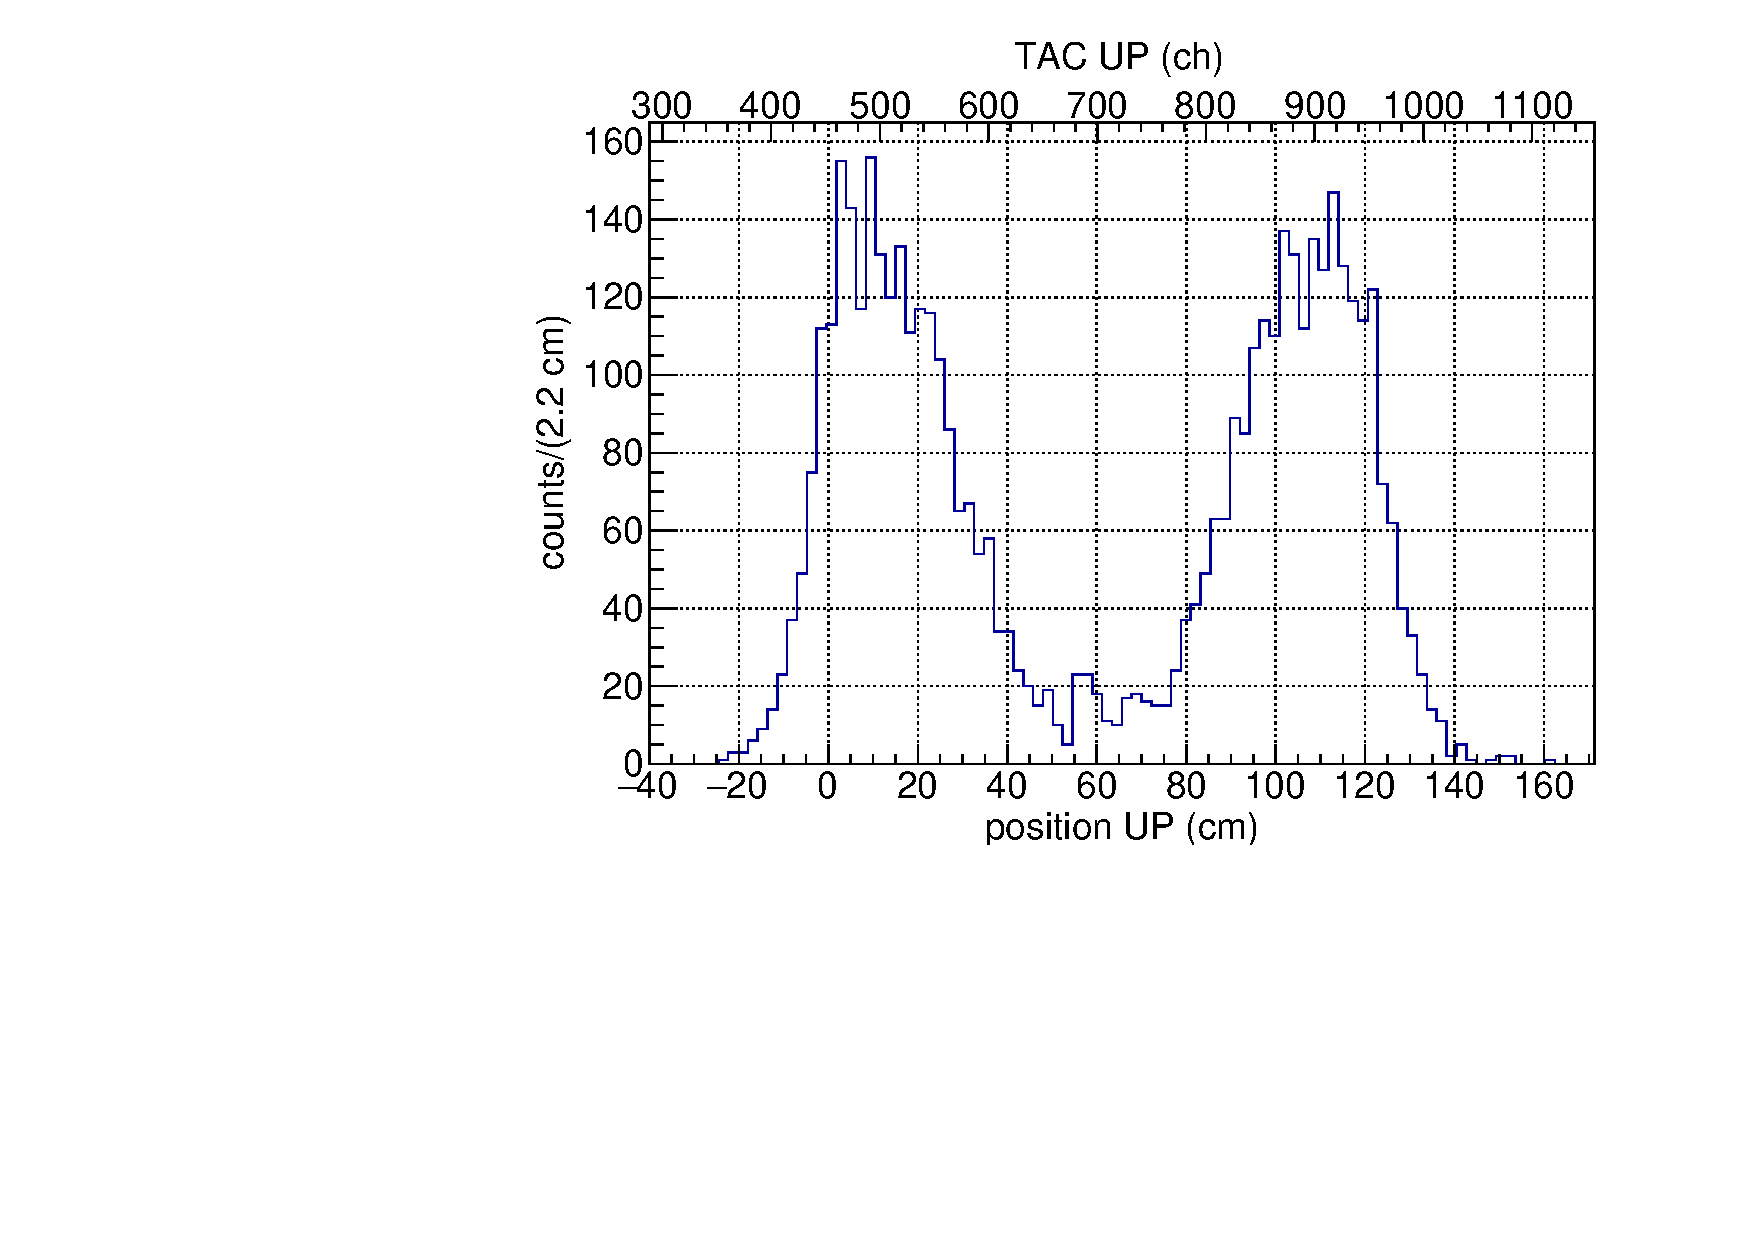
\includegraphics[width=0.48\linewidth]{Figures_TACs/Calibration_up.pdf}}
   % \hspace{-0.5 cm}
   %  \subfloat[][DOWN]
     {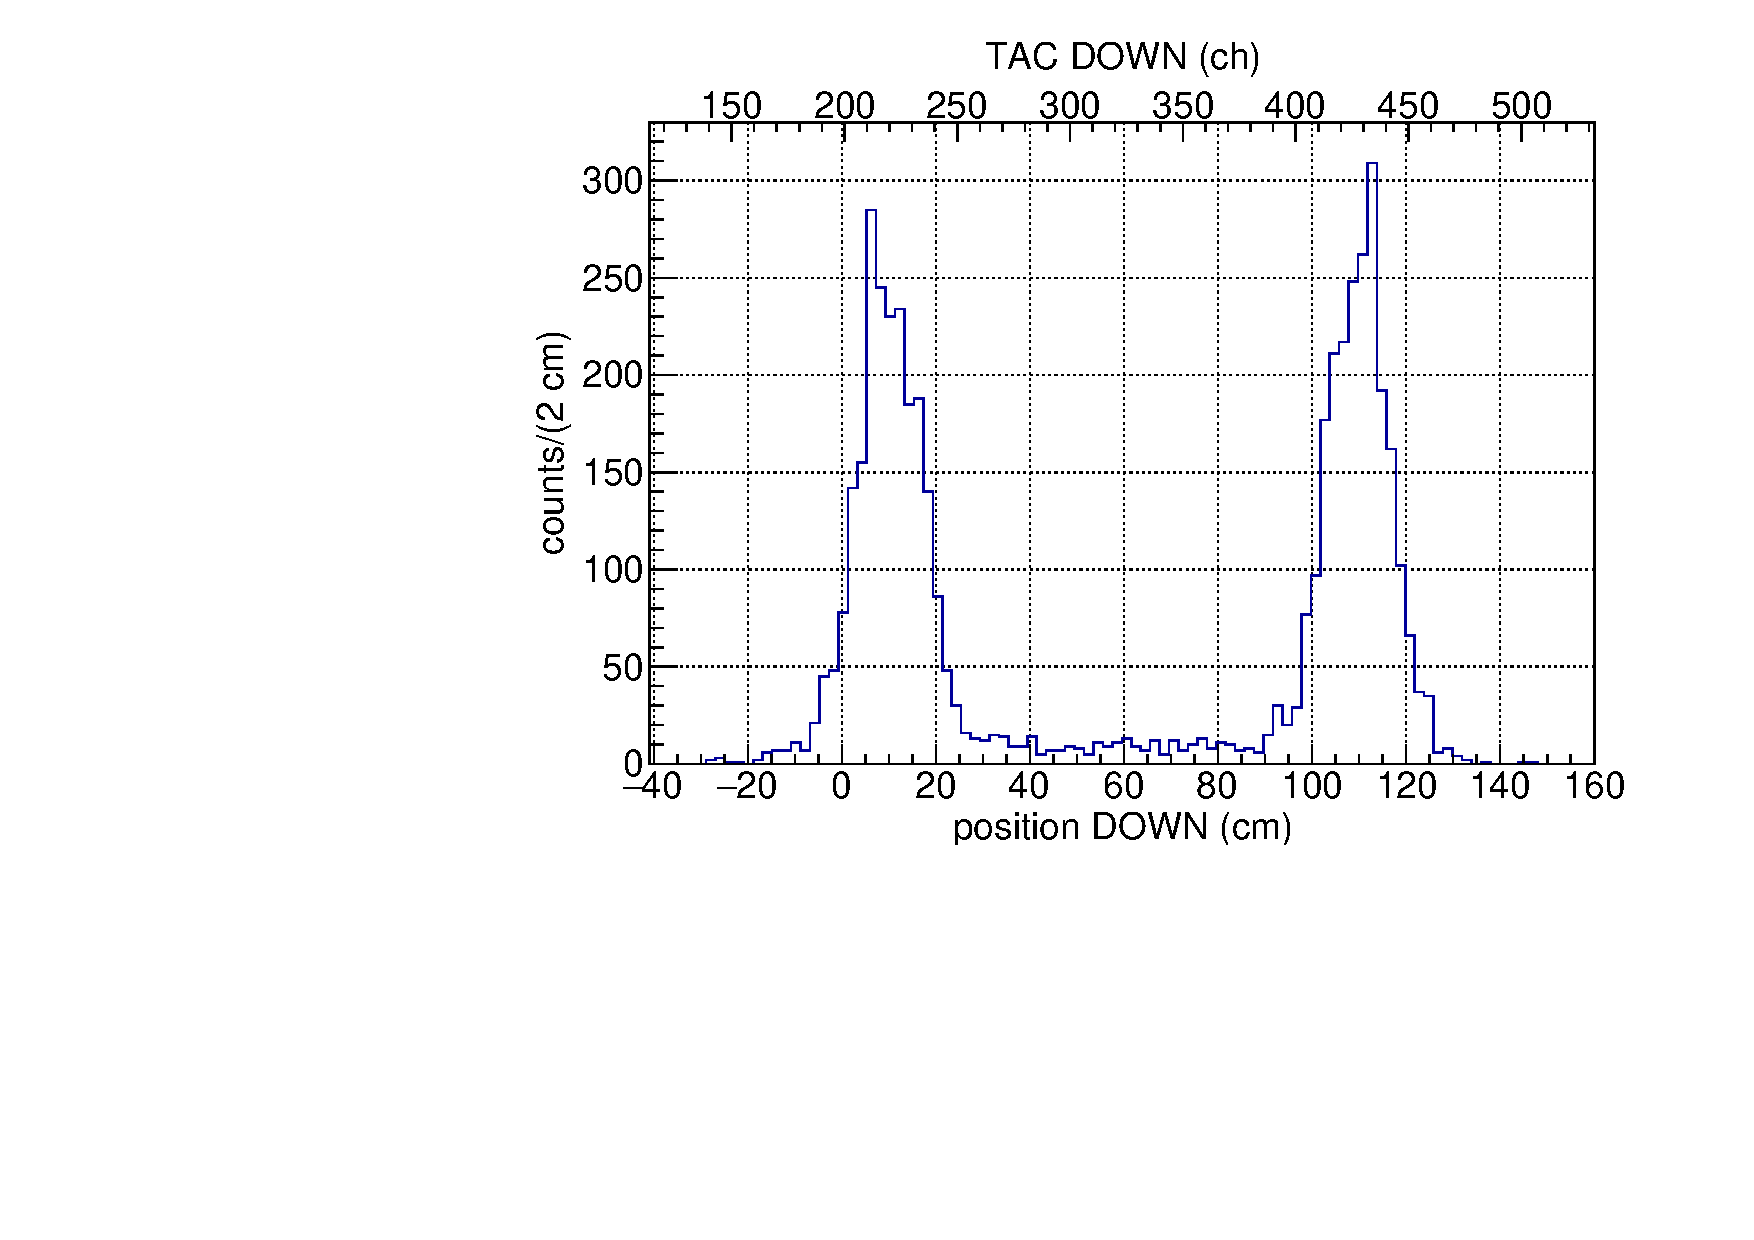
\includegraphics[width=0.48\linewidth]{Figures_TACs/Calibration_down.pdf}}
     %\caption{Events in coincidence with the trackers in scintillator \textbf{(a)} UP, \textbf{(b)} DOWN. The upper x-axis represents the original FPGA measure of the output of the TAC, while the lower x-axis is calibrated in position.}
     \caption{Events in coincidence with the trackers in scintillator UP (on the left) and DOWN (right). The upper x-axis represents the original FPGA measure of the output of the TAC, while the lower x-axis is calibrated in position.}
    \label{fig:position calibration}
\end{figure}

\vspace{-0.5cm}
\begin{table}[H]
    \centering
   % \captionsetup{width=.7\linewidth}
    \begin{tabular}{|c|cc|}
    \hline
       $x$ (cm)  & $C_\mathrm{UP}$ (ch) & $C_\mathrm{DOWN}$ (ch)  \\
       \hline
       10  & $494\pm2$ &$219.8\pm0.3$\\
       110 & $905\pm2$ & $428.1\pm0.3$\\
       \hline
    \end{tabular}
    \caption{Positions $x$ of the trackers and corresponding centroids $C$ in the UP and DOWN TAC spectra}
    \label{tab:position cal}
\end{table}
\vspace{-0.25cm}
\begin{figure}[H]
    \centering
    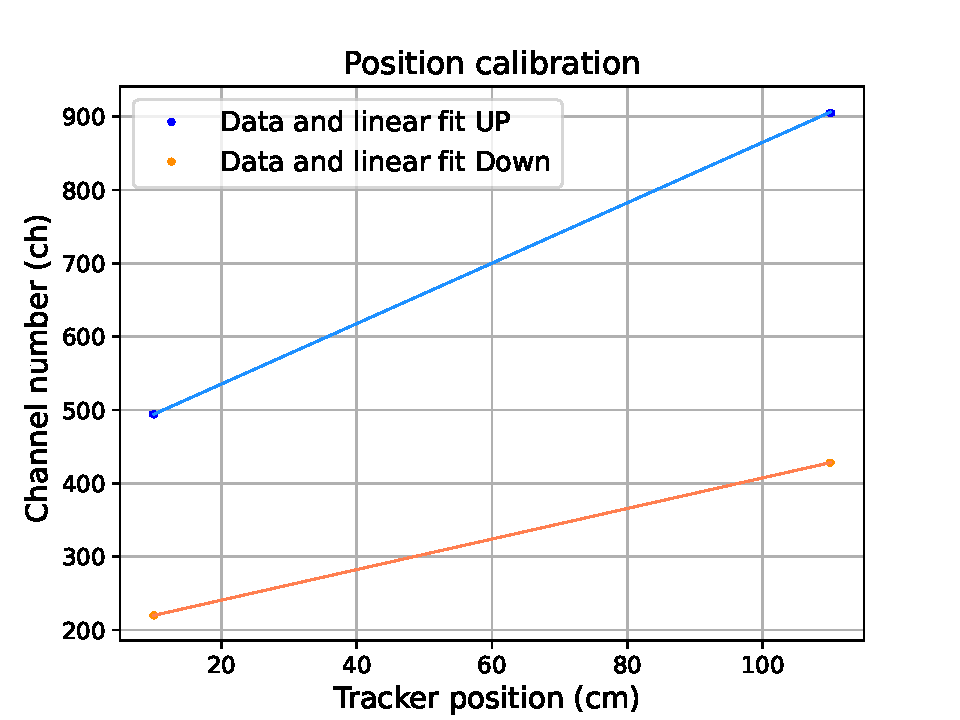
\includegraphics[width=0.48\linewidth]{linear_graph/position_cal.pdf}
    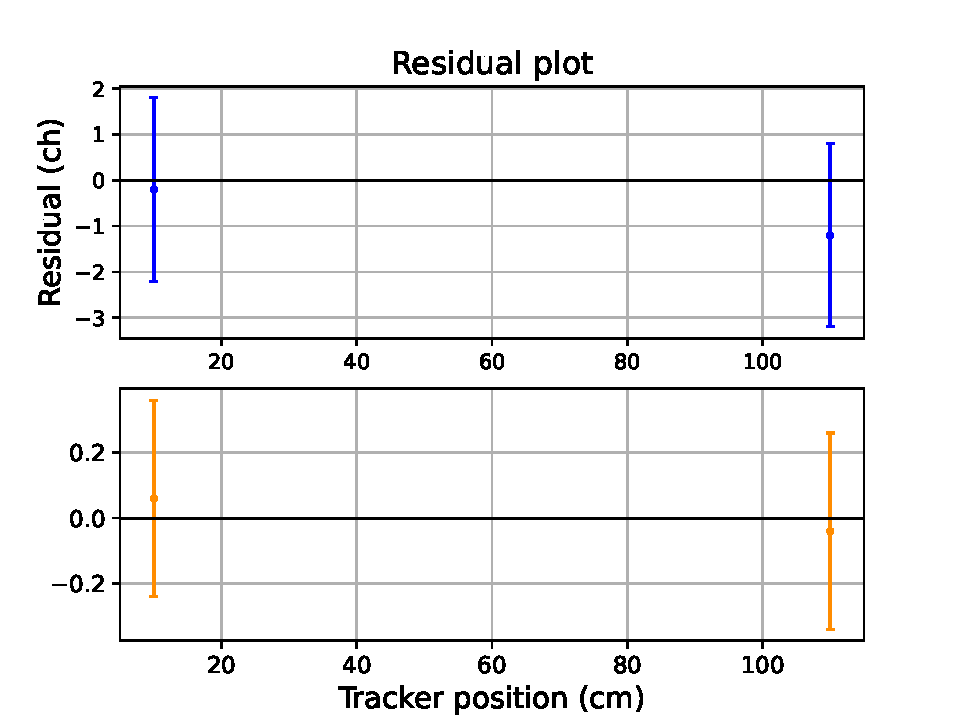
\includegraphics[width=0.48\linewidth]{linear_graph/position_cal_res.pdf}
    \caption{Position calibration of TAC UP (blue) and TAC DOWN (orange) and residuals: on the x-axis the positions $x$ and on the y-axis the centroids $C$ (see Tab. \ref{tab:position cal})}
    \label{fig:linear fit for position cal}
\end{figure}

\vspace{-0.25cm}
\begin{figure}[H]
    \centering
    %\subfloat[][UP]
    {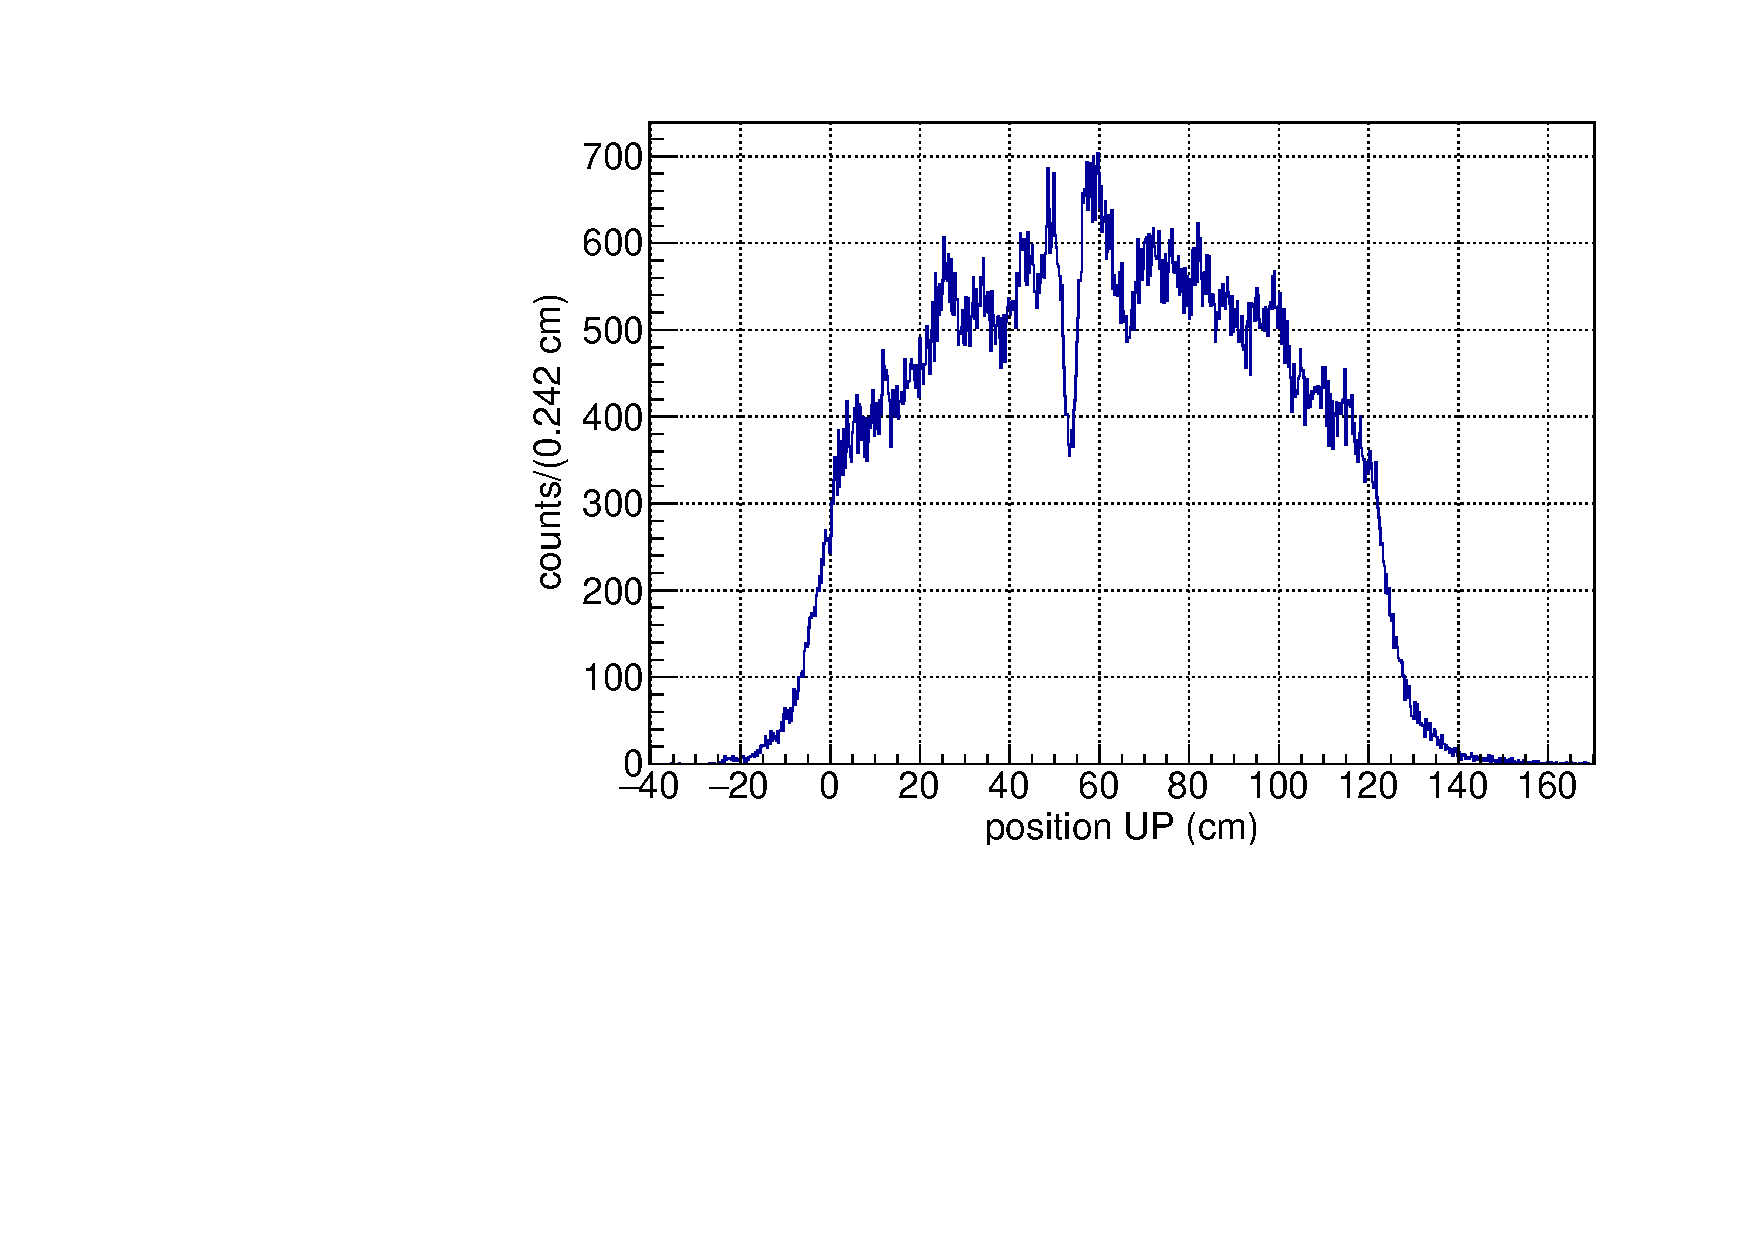
\includegraphics[width=0.48\linewidth]{Figures_TACs/spectrum_UP3.pdf}}
    %\hspace{-0.5 cm}
     %\subfloat[][DOWN]
     {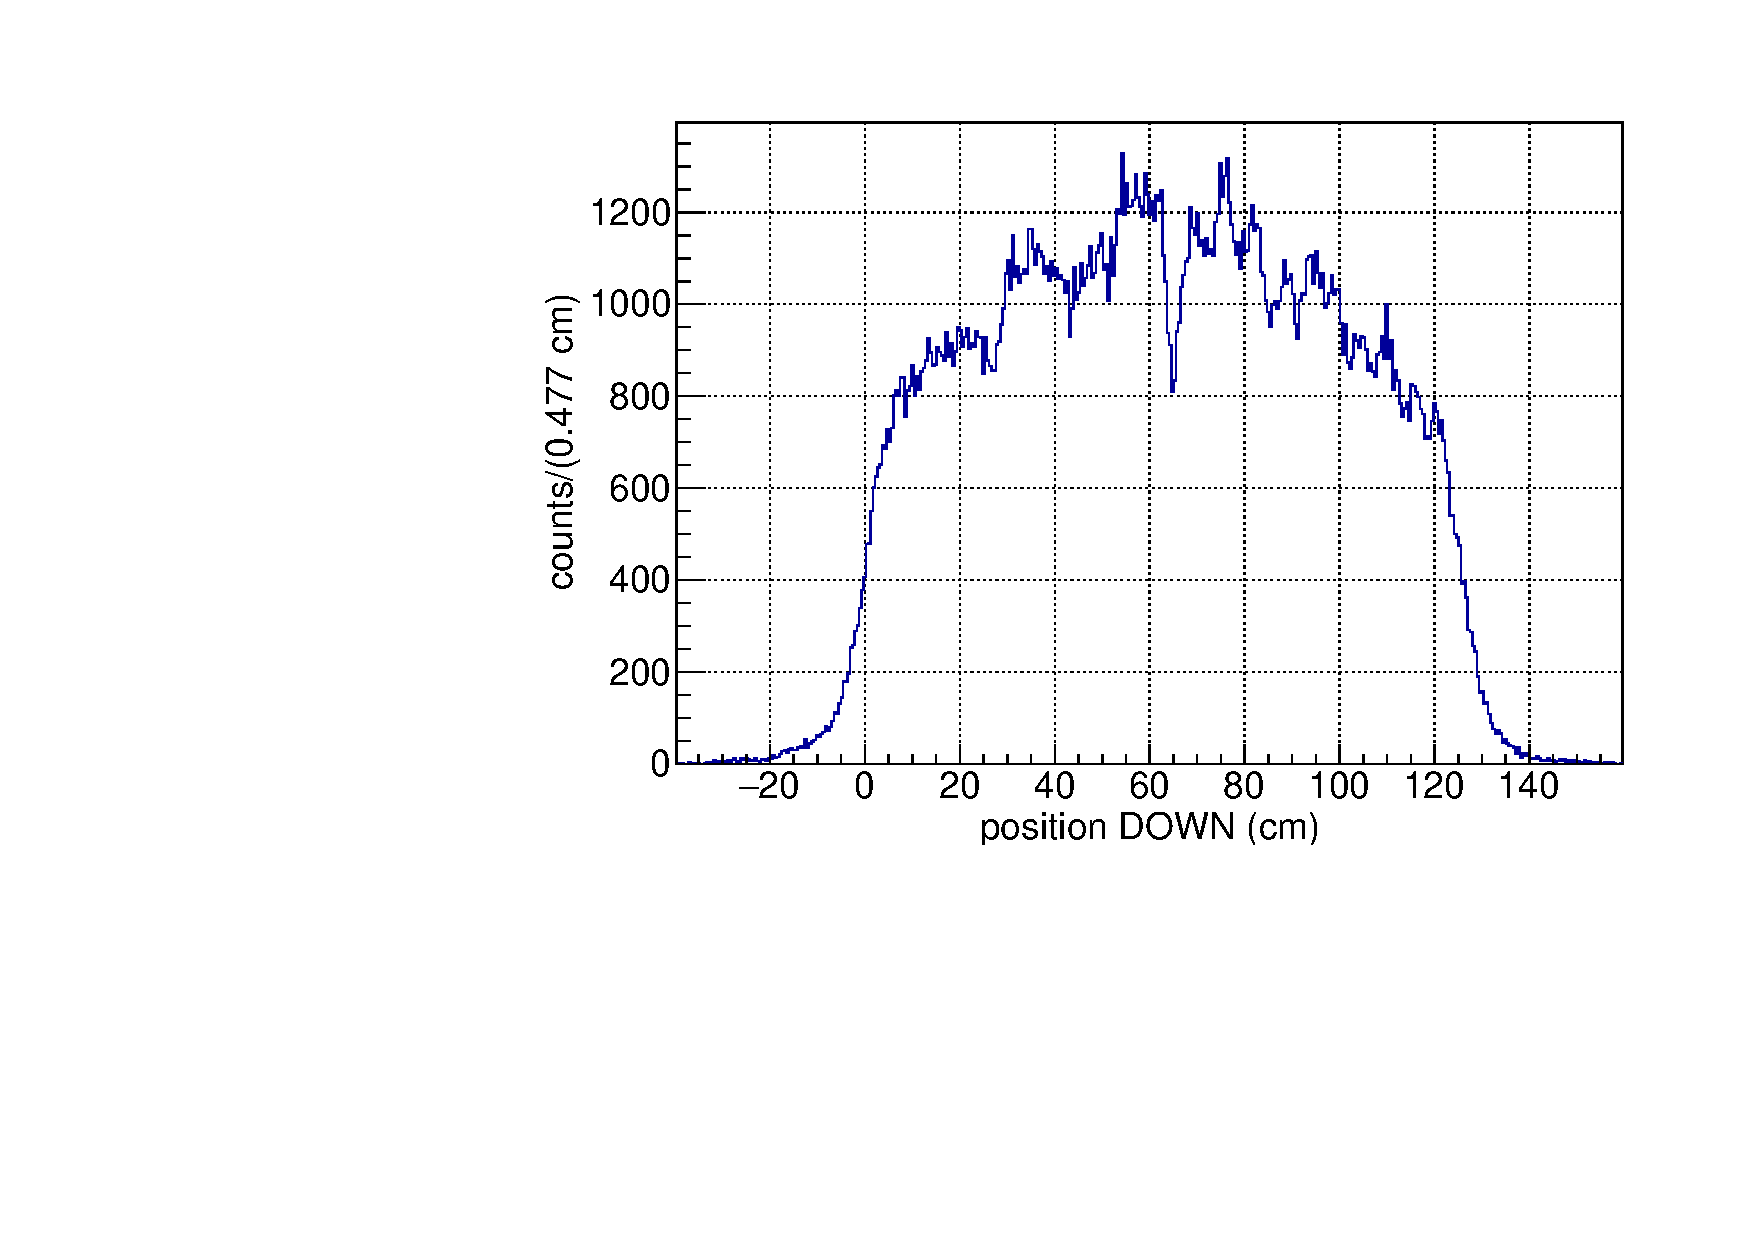
\includegraphics[width=0.48\linewidth]{Figures_TACs/spectrum_DOWN3.pdf}}
     %\caption{Position-calibrated spectra from \textbf{(a)} TAC UP, \textbf{(b)} TAC DOWN} 
    \caption{Position calibrated spectra from TAC UP and TAC DOWN} 
    \label{fig:calibrated spectra position}
\end{figure}

Since the horizontal dimensions of the trackers are finite, for geometrical reasons not a single muon direction but a whole set of muon directions is selected by the $\mathtt{T_1}$ (or $\mathtt{T_2}$) coincidence. %Considering for simplicity only the longitudinal degree of freedom, the range of muon directions that cross \textit{both} tracker UP and tracker DOWN is the one delimited by two lines: the line matching the left end of the longitudinal side of tracker UP to the right end of the DOWN one and the line matching the right UP end to the left DOWN end. The widths of the peaks in the position-calibrated spectra are then proportional to the distance of the respective scintillator (UP or DOWN) from the midpoint between the UP and DOWN trackers. 
In the setup of the experiment, the internal semi-width of the peaks is expected to be $\approx\!34$ cm in the UP scintillator and $\approx\!12$ cm in the DOWN scintillator\footnote{The external side of the peak has a lower extension with respect to the internal one because the scintillator ends.} (see Fig. \ref{fig:scheme}). 
The calibrated coincidence peaks in Fig. \ref{fig:position calibration} agree with these estimates.% \textcolor{red}{io aggiungerei lo schema in piccolo}

\begin{figure}[H]
    \centering
    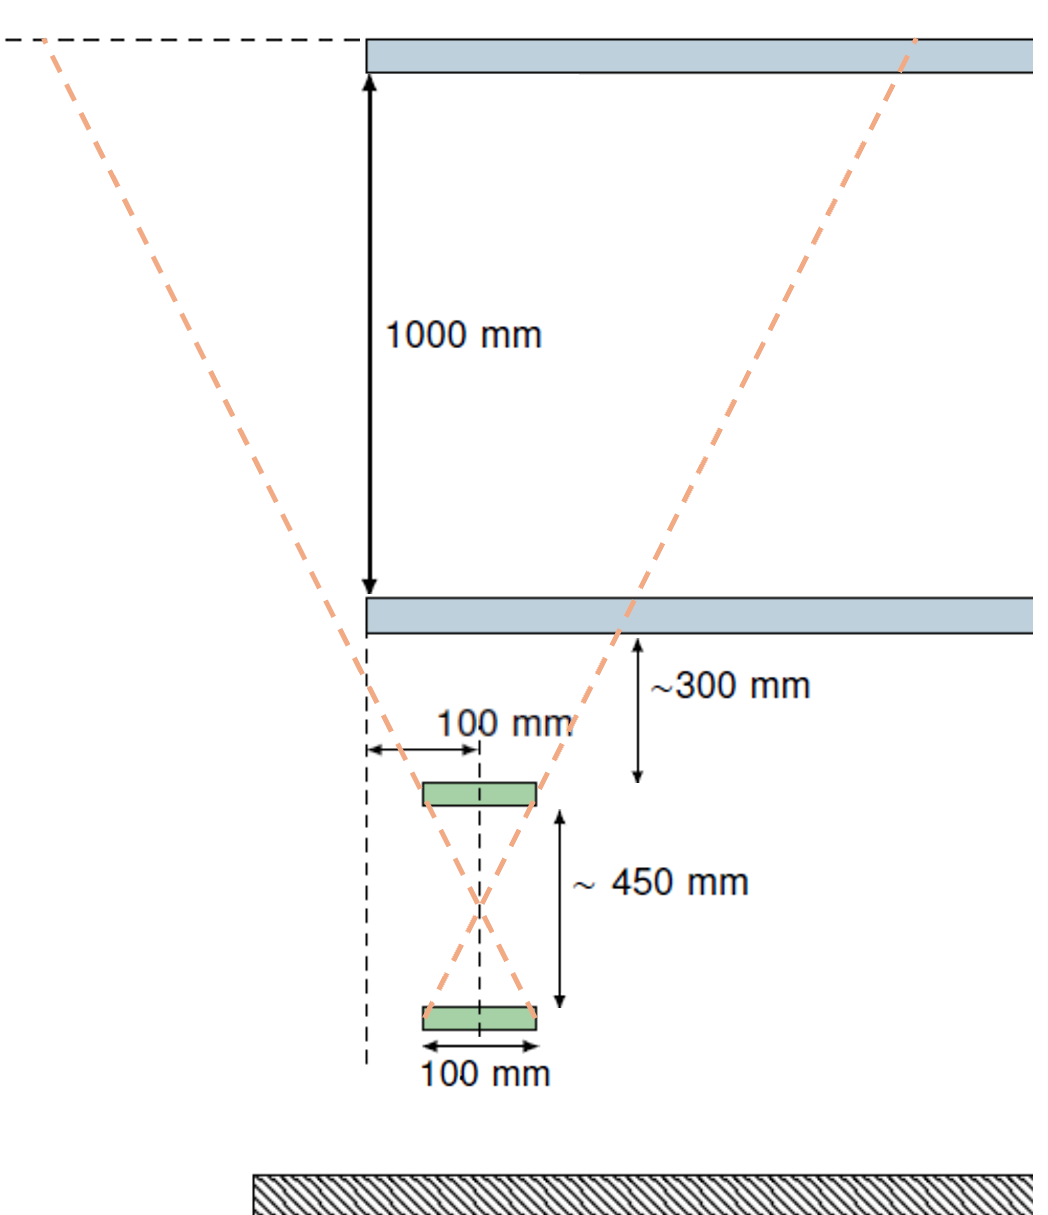
\includegraphics[height=0.45\linewidth]{Scheme/Immagine1.png}
    \caption{Considering for simplicity only the longitudinal degree of freedom, the range of muon directions that cross \textit{both} tracker UP and tracker DOWN is the one delimited by two lines. %: the line matching the left end of the longitudinal side of tracker UP to the right end of the DOWN one and the line matching the right UP end to the left DOWN end. 
    The widths of the peaks in the position-calibrated spectra are then proportional to the distance of the respective scintillator (UP or DOWN) from the midpoint between the UP and DOWN trackers.}
    \label{fig:scheme}
\end{figure}

Let us notice that, according to the \textit{time} calibrations of TAC UP and TAC DOWN (Sect. \ref{sect:time calibration}), the time difference between the two centroids of the same spectrum (Fig. \ref{fig:position calibration}) turns out to be $(13.8\pm0.2)$ ns and $(14.0\pm0.2)$ ns for TAC UP and TAC DOWN, respectively. 
If the path of scintillation light is approximated as a straight line in the longitudinal direction, these time differences are expected to be in the vicinity of \[\frac{2(x_2-x_1)}{v_\mathrm{s}}\approx14\,\mathrm{ns}\] where $v_\mathrm{s}\approx\tfrac{1\,\mathrm{m}}{7\,\mathrm{ns}}$ is an average speed of scintillation light inside the scintillators\footnote{Indeed, the TAC time measure corresponds to Eq. \eqref{eq: time measured by tac up and down} and the following holds:
% If we approximate the path of scintillation light as a straight line in the longitudinal direction, we get the following relation between the time 
$ t_{\mathrm{left}}^{(i)}-t_\mathrm{right}^{(i)}\approx \tfrac{x^{(i)}}{v_\mathrm{s}}-\tfrac{L-x^{(i)}}{v_\mathrm{s}}=\tfrac{2x^{(i)}-L}{v_\mathrm{s}},\quad \quad i=\mathrm{UP,\,DOWN.}$}. Hence, the estimates are compatible with the expected value within $1\sigma$.\\ %, whereas the TAC UP one is 10\% higher. The cause may be a slight inaccuracy either in determining the peaks' positions in the histogram of Fig. \ref{fig:position calibration} or in calibrating TAC UP in time.
 
Finally, it is possible to check the correlation between the measured position of the trackers and the corresponding time difference between the DOWN detector and the UP detector, shown in Fig. \ref{fig:time D-U vs position}. As expected, the events recorded by the trackers have roughly the same time difference between the UP detector and the DOWN detector, because the trajectory of those muons is almost perpendicular to the scintillators. 

\vspace{-0.4cm}
\begin{figure}[H]
    \centering
    %\subfloat[][UP]
    {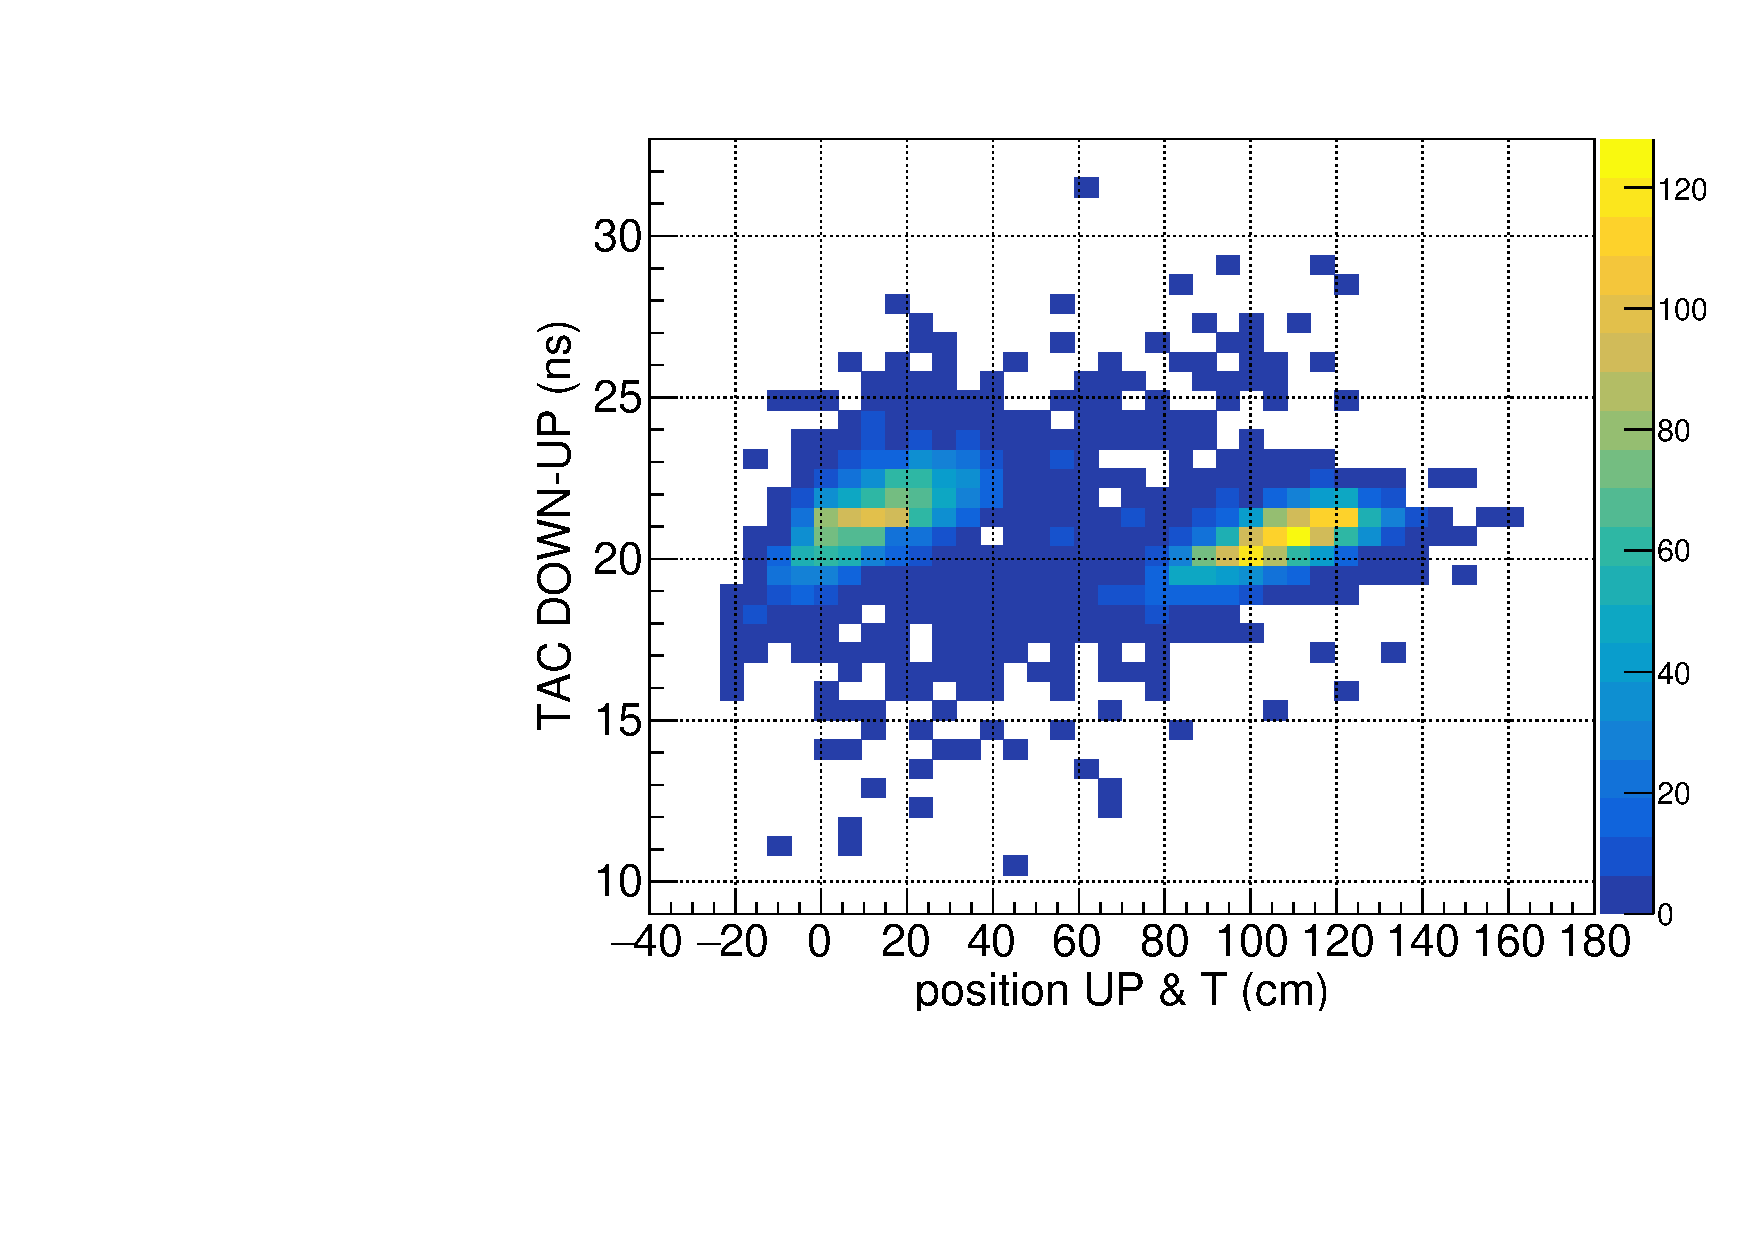
\includegraphics[width=0.4\textwidth]{Figures_TACs/time_DU_vs_U.pdf}} \quad\quad\quad
   % \hspace{0.4 cm}
    % \subfloat[][DOWN]
     {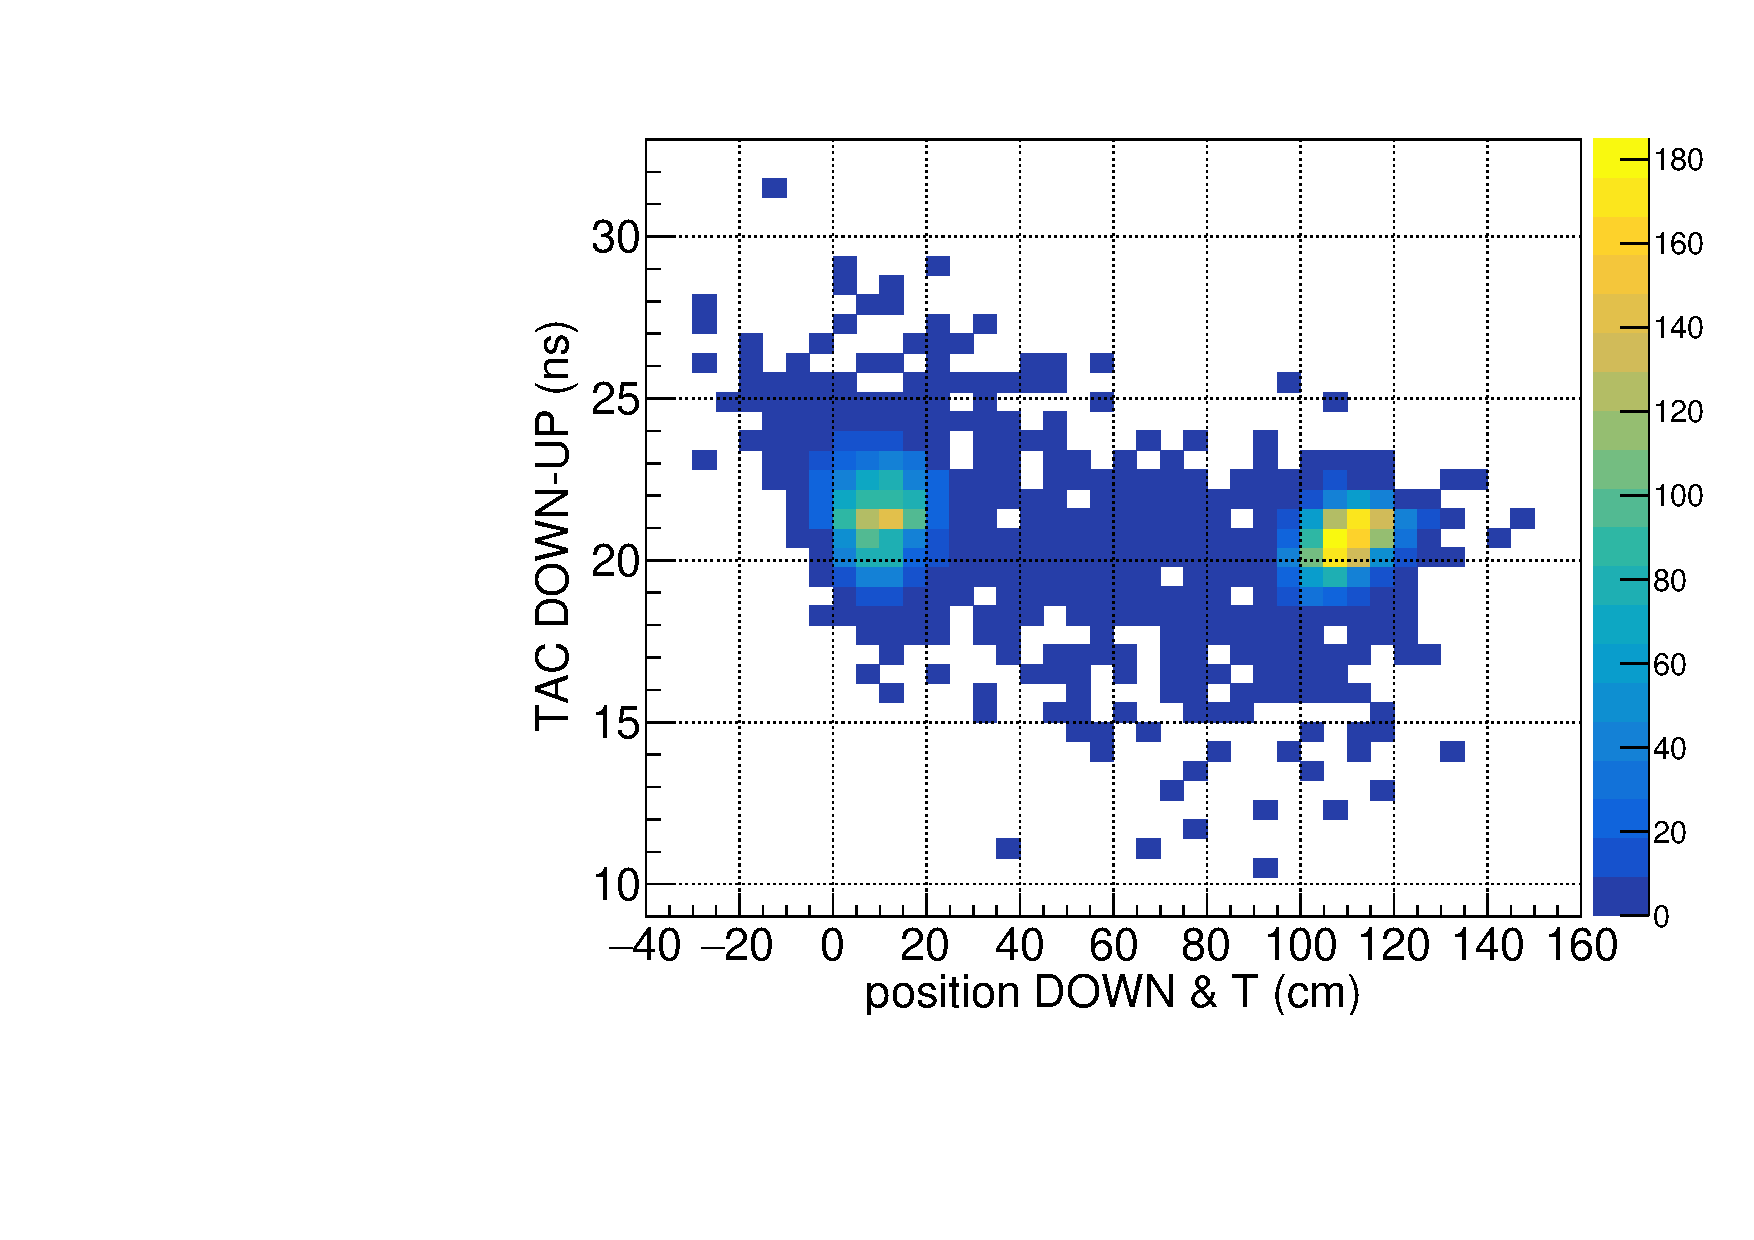
\includegraphics[width=0.4\textwidth]{Figures_TACs/time_DU_vs_D.pdf}}
     \caption{Correlation between the measured position and the time DOWN-UP: in both graphics the time measurement of the two peaks is the same; furthermore, comparing the two graphics, the time measurement is in agreement also for both UP and DOWN position.} 
    \label{fig:time D-U vs position}
\end{figure}


\subsubsection{Study of the correlation between TACs measurements}
\paragraph{1. DOWN position vs UP position}\hypertarget{DOWN vs UP}{}
Let's now study the correlation between the position UP $x_\mathrm{U}$ and the position DOWN $x_\mathrm{D}$. Indeed, the expected impact position of muons on the lower scintillator $x_\mathrm{D}$, assuming that their path is not changed and neglecting the thickness of the two scintillators, is given by the equation
\begin{equation}
    x_\mathrm{D}\approx x_\mathrm{U}+d\,\tan\alpha, \quad\alpha\in\big[\arctan(-\tfrac{x_\mathrm{U}}{d}),\,\arctan(\tfrac{L-x_\mathrm{U}}{d})\big]
\end{equation}
where $d$ is the spacing between the two scintillators and $\alpha$ is the angle of the muon direction with respect to the vertical in $x\!=\!x_\mathrm{U}$.

\begin{figure}[H]
    \centering
    %\subfloat[][]
    {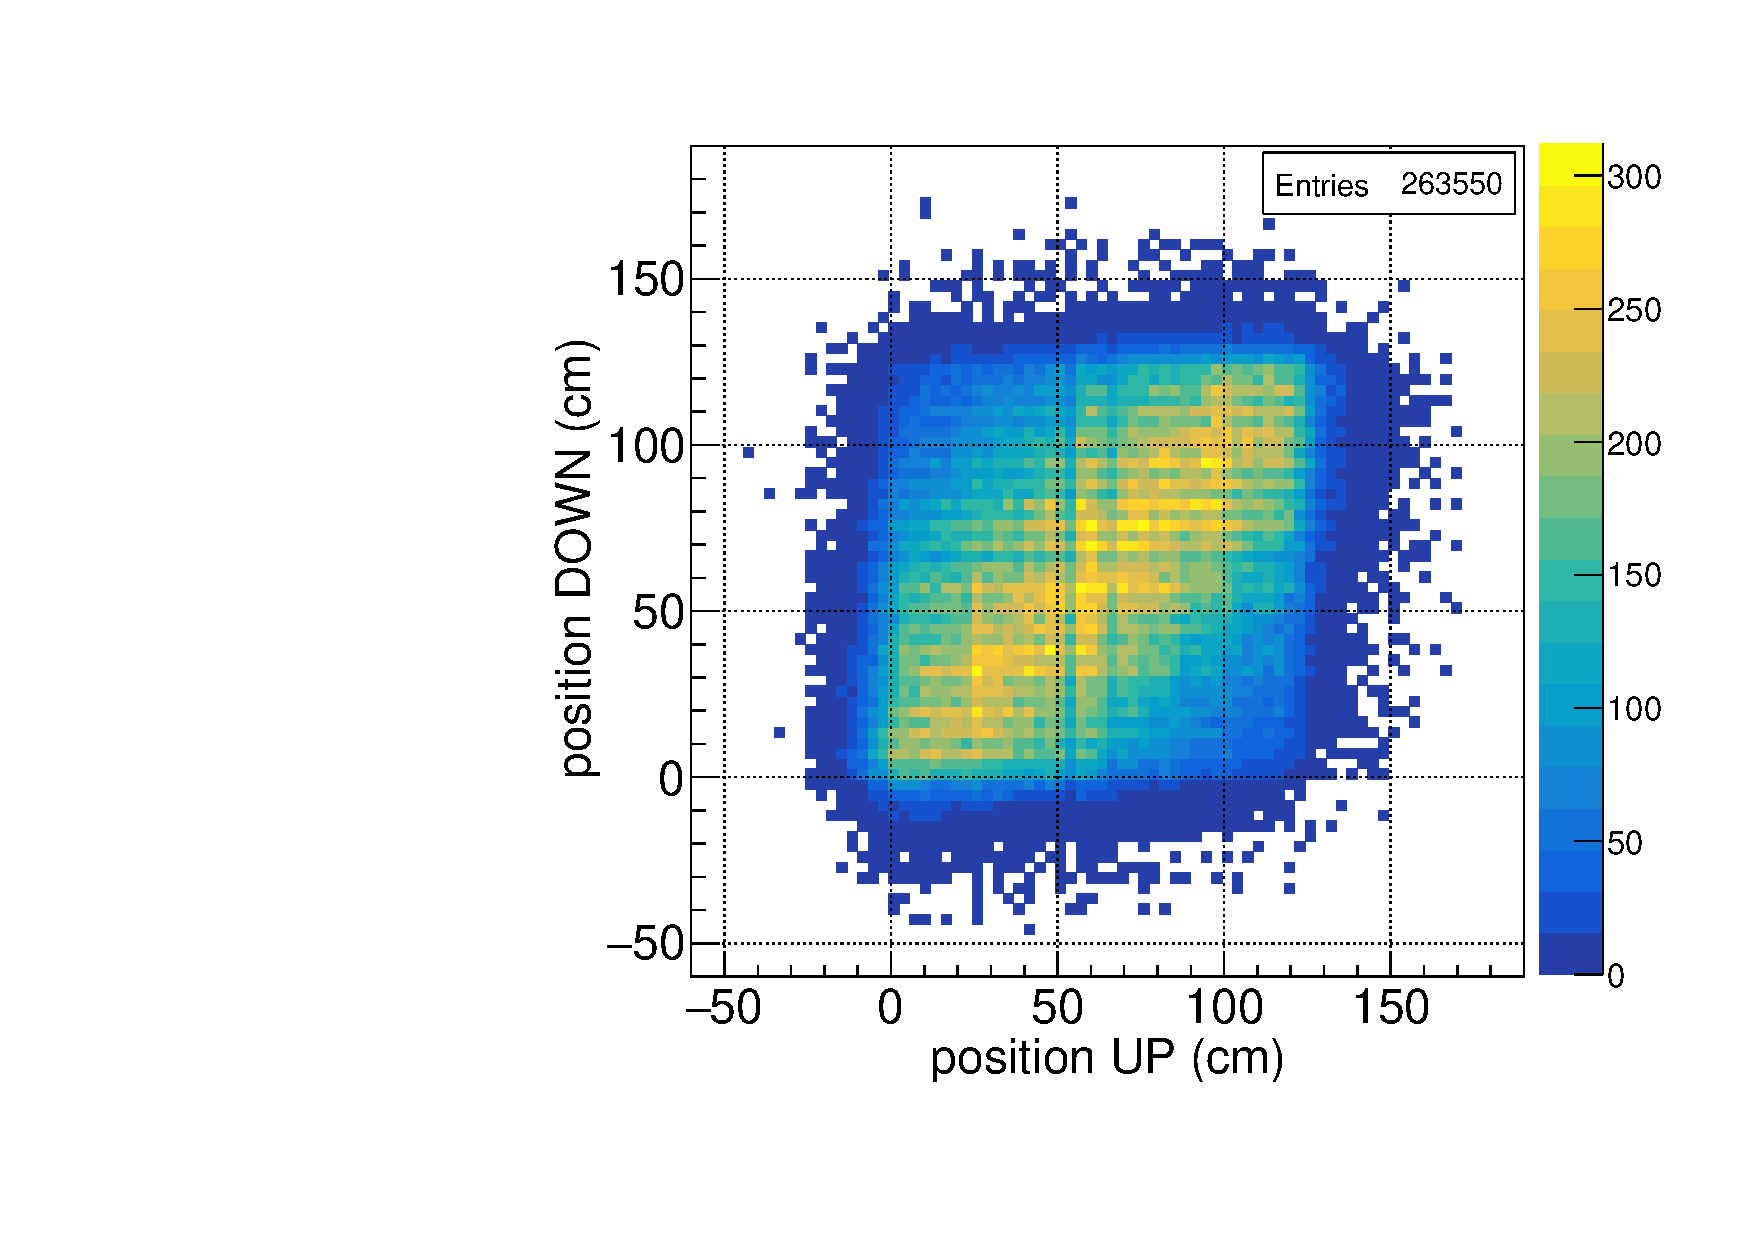
\includegraphics[width=0.48\linewidth]{Figures_Correlations/d-u3.pdf}}
    \hspace{-0.1 cm}
   %  \subfloat[][]
     {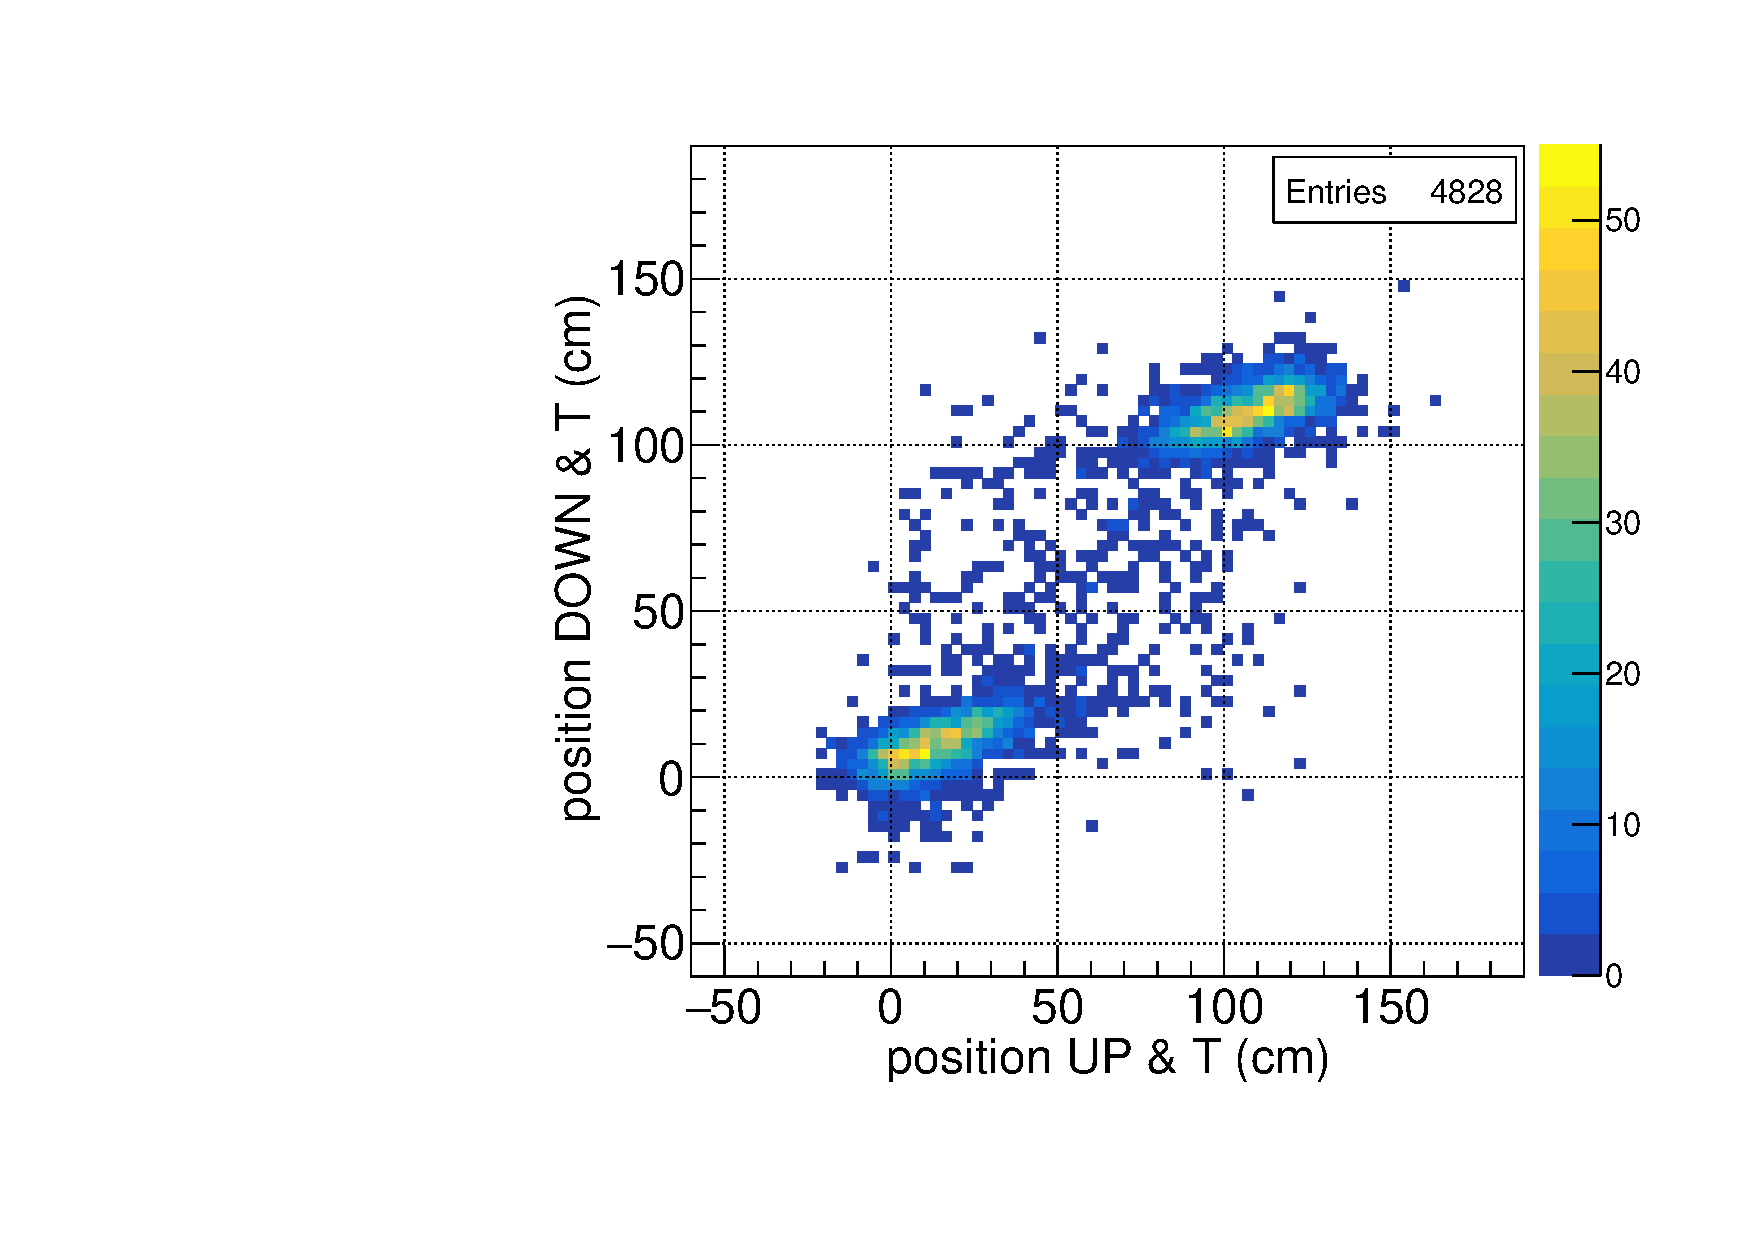
\includegraphics[width=0.48\linewidth]{Figures_Correlations/peaks.pdf}}
     \caption{Correlation between impact positions of the muons on upper and lower scintillator: on the left, the two spectra of UP and DOWN position; on the right, the same spectra including only the events in coincidence with the trackers.} 
    \label{fig:down vs up}
\end{figure}


%\vspace{3mm}
In the first graphic in Fig. \ref{fig:down vs up}, both the position spectra calibrated for UP and DOWN scintillators, already shown in Fig. \ref{fig:calibrated spectra position}, are plotted in a 2D histogram, respectively on the x-axis and the y-axis. As expected, a positive correlation is clearly visible.

Instead, in the graphic on the right, the two spectra of position, already calibrated, including only the events in coincidence with the trackers (Fig. \ref{fig:position calibration}), define two peaks, showing again the correlation between the impact positions of muons on UP and DOWN scintillators.
\paragraph{2. DOWN position as the UP position is fixed}
The relationship between position DOWN and position UP can be further investigated by checking the distribution of $x_\mathrm{D}$ (i.e. $ \tfrac{\mathrm{d}N}{\mathrm{d}x_\mathrm{_D}}$) for events whose $x_\mathrm{U}$ belongs to a small region, which accounts for "fixing $x_\mathrm{U}$". 
Let us plot in Fig. \ref{fig:down for up small} the distribution of $x_\mathrm{D}$ as $x_\mathrm{U}\in[25;35]$ cm (blue) and $x_\mathrm{U}\in[85;95]$ cm (red). 
In the first case, the particles impact near the UP PMT on the left, in the second case they impact near the UP right PMT. 
It may be seen clearly that the distributions reach their peak at the position $x_\mathrm{D}$ that is normal to the selected position $x_\mathrm{U}$.
\begin{figure}[H]
    \centering
    \captionsetup{width=.85\linewidth}
    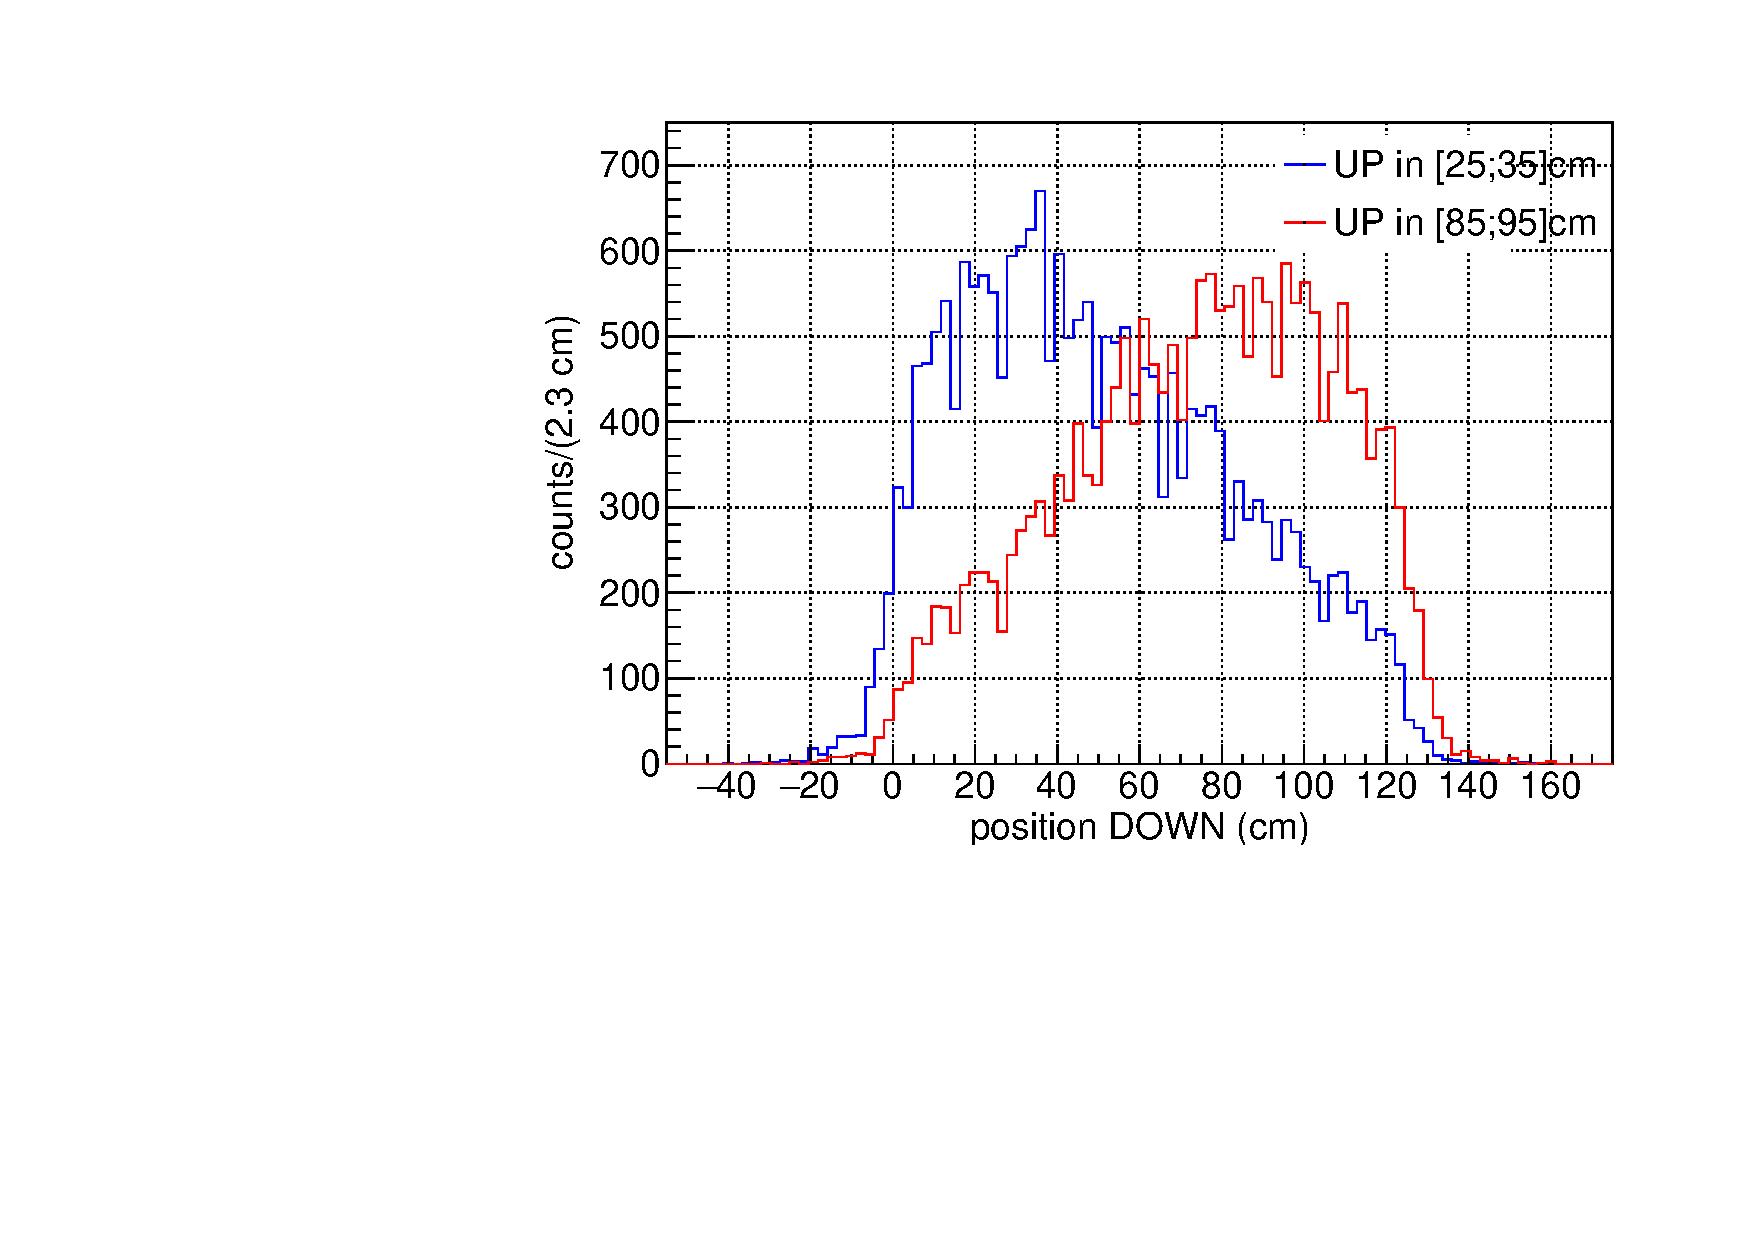
\includegraphics[width=0.6\linewidth]{Figures_Correlations/DOWN_UPsmall2.pdf}
    \caption{Distribution of position DOWN ($x_\mathrm{D}$) as the position UP ($x_\mathrm{U}$) belongs to two different small intervals}
    \label{fig:down for up small}
\end{figure}

When considering only the longitudinal position (i.e., neglecting the coordinate corresponding to the width of the scintillators), the expected analytical expression for the distribution is 
% \textcolor{blue}{(To be completed with the other angle?)} %we can just say that for semplicity we are considering just this angle, but that a further analysis can be done adding the solid angle.
\begin{equation}
    \frac{\mathrm{d}N}{\mathrm{d}x_\mathrm{D}}\bigg|_{x_\mathrm{U}}= \frac{\mathrm{d}N}{\mathrm{d}\alpha}\frac{\mathrm{d}\alpha}{\mathrm{d}x_\mathrm{D}}\bigg|_{x_\mathrm{U}}= \frac{\mathrm{d}N}{\mathrm{d}\alpha}\,\frac{1}{d\,(1+\tan^2\alpha)}= \frac{\mathrm{d}N}{\mathrm{d}\alpha}\,\frac{d}{d^2+(x_\mathrm{D}-x_\mathrm{U})^2}
\end{equation}
where $\alpha$ and $d$ are the quantities described in the paragraph \hyperlink{DOWN vs UP}{"DOWN vs UP"}. This function does have a maximum as $x_\mathrm{D}=x_\mathrm{U}$, in line with both Fig. \ref{fig:down vs up} and Fig. \ref{fig:down for up small}. 


\paragraph{3. DOWN-UP time vs. DOWN position as the UP position is fixed}
The same selections of events as in the previous paragraph can be used to study the correlation between the DOWN-UP time measurement and position DOWN. Indeed, the time spectrum of the DOWN-UP TAC is given by the sum of three terms (Eqn. \ref{eqn: spectra}): the first one is the time required for the muon to reach the lower scintillator (with an average speed $v_\mu\approx30 \,\mathrm{cm/ns}$), the second is the time difference for the light produced in the scintillator to propagate up to the right side and the third one the delay already discussed before (Sect. \ref{sect:time calibration})
\begin{equation} \label{eqn: spectra}
    \Delta t^\mathrm{(D-U)}= %\frac{d}{v\,\cos\alpha}+\frac{x_\mathrm{U}-x_\mathrm{D}}{v_\mathrm{s}}+T_d^\mathrm{(D-U)}= 
    \frac{\sqrt{d^2+(x_\mathrm{D}-x_\mathrm{U})^2}}{v_\mu}+\frac{x_\mathrm{U}-x_\mathrm{D}}{v_\mathrm{s}}+T_d^\mathrm{(D-U)}
\end{equation}

Therefore, in the next graphics this relation is studied by plotting the position DOWN distribution, obtained in Fig. \ref{fig:calibrated spectra position}, on the x-axis and the DOWN-UP time spectrum (third picture in Fig. \ref{fig:tac time spectra}) on y-axis; the graphic on the left refers to $x_\mathrm{U}\in\left[25;35\right]$ cm, whereas the one on the right to $x_\mathrm{U}\in\left[85;95\right]$ cm.


%\textcolor{blue}{%We should say that $v_\mu$ is roughly 30 cm/ns. 
%In case we want to, we may add the theoretical function in the pictures of Fig. 14, otherwise we may say "when plotting the theoretical function without showing it..." }

When plotting the theoretical function (Eqn. \ref{eqn: spectra}), it's possible to recognize the same decreasing trend.  %andamento
However, a proper fit in this case will not be provided because of the several approximations in the parameters of the function. Let's also notice that the negative correlation is confirmed.

\begin{figure}[H]
    \centering
    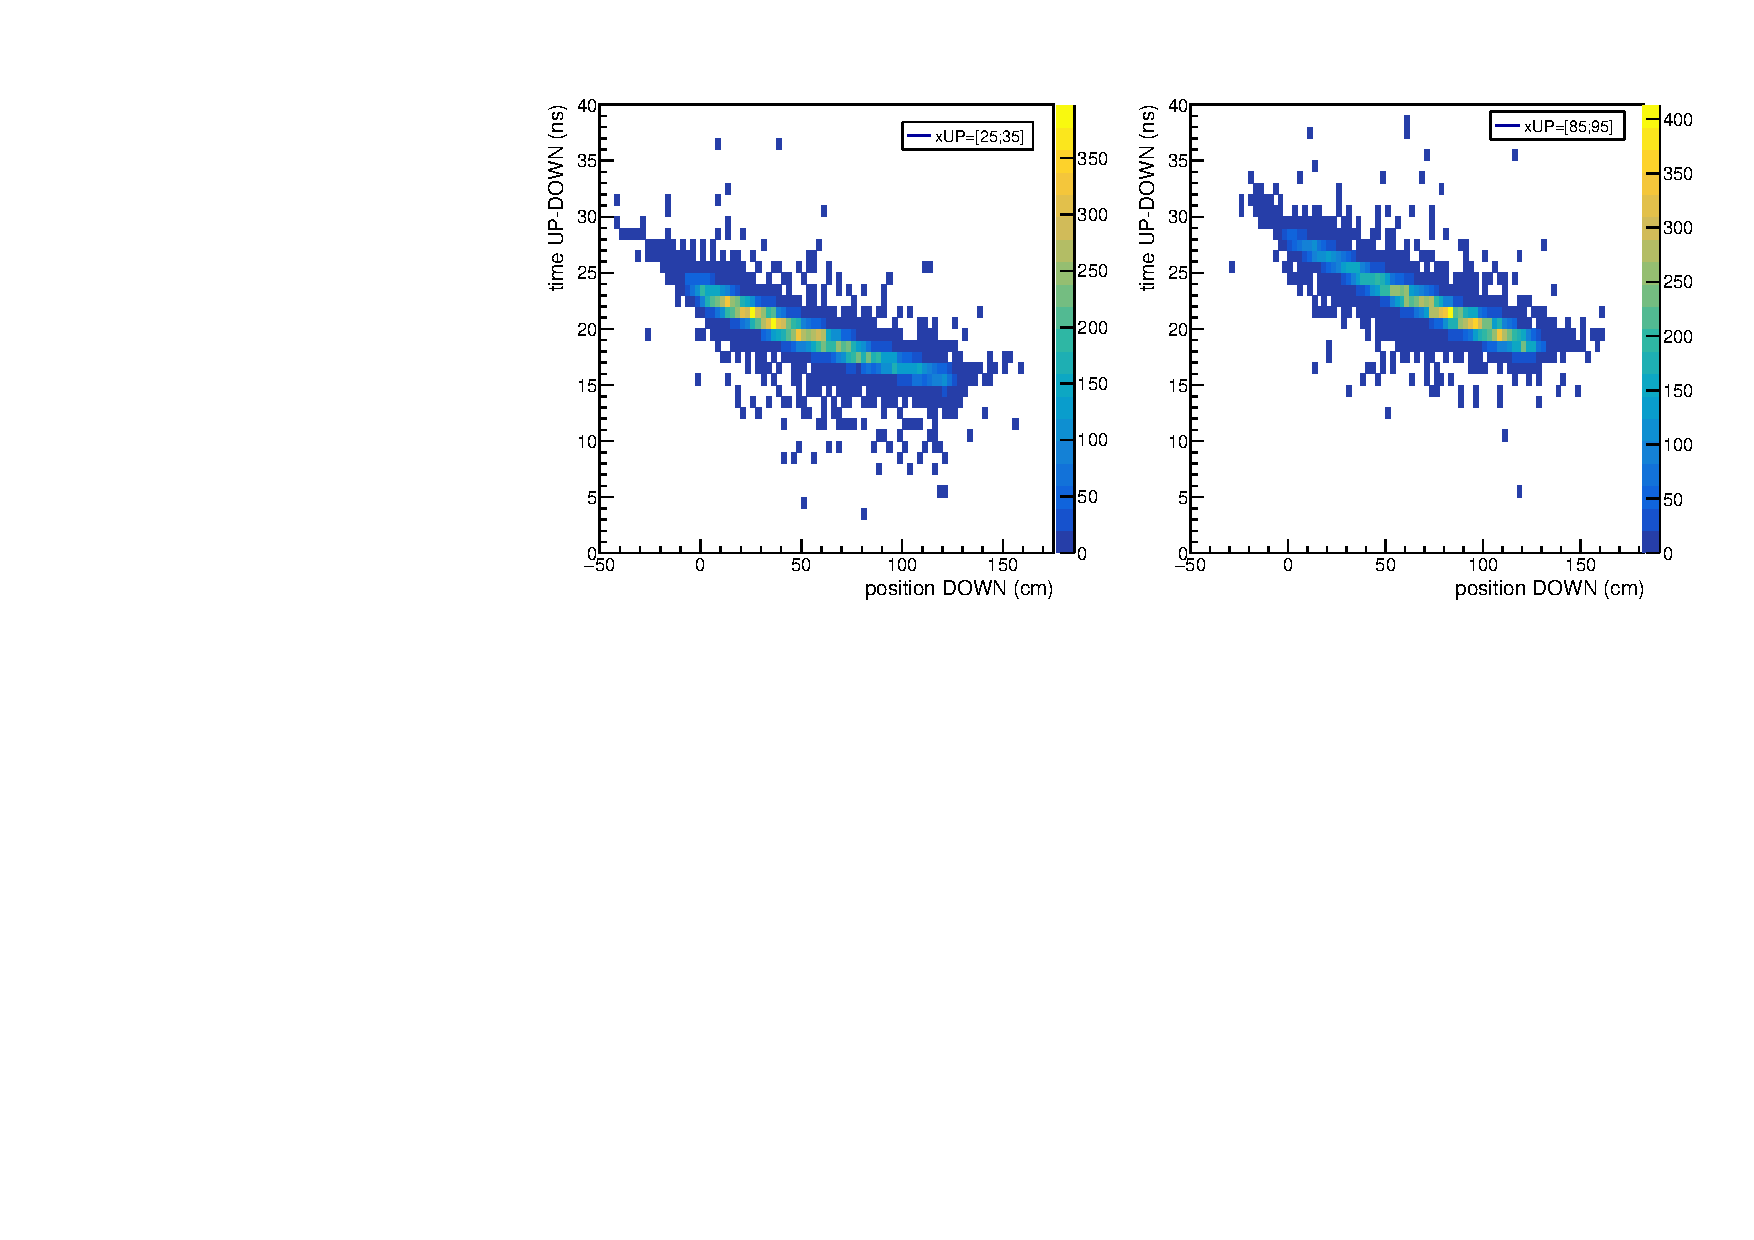
\includegraphics[width=\linewidth]{hint5.pdf}
    \caption{Correlation between time spectrum DOWN-UP and position spectrum DOWN constrained on the upper position: $x_\mathrm{U}\in[25;35]$ cm (on the left), $x_\mathrm{U}\in[85;95]$ cm (on the right). Again it's possible to observe a peak for $x_\mathrm{D}\simeq x_\mathrm{U}$.}
    \label{fig:hint5}
\end{figure}


\subsubsection{Efficiency measurement} 
\hypertarget{efficiency}{}
The efficiency of the telescope with respect to the trackers is defined as 
$$r\equiv\dfrac{N_{\mathtt{UP \wedge DOWN \wedge (T_1 \vee\, T_2)}}}{N_\mathtt{(T_1 \vee \,T_2)}}$$
where $N_{\mathtt{UP \wedge DOWN \wedge (T_1 \vee\, T_2)}}$ is the number of events seen both by the trackers and the pair of detectors, while $N_\mathtt{(T_1 \vee \,T_2)}$ is the number of events measured just by the trackers in the same time interval. 
 
Using the CAEN scaler, the rate of $\mathtt{T=T_1\vee T_2}$ events was measured as explained in the third paragraph of Sect. \hyperlink{2.1.2}{2.1.2}, where the rate estimate has been shown. Thus, in $1\,\mathrm{s}$ the number of recorded events is:
 $$N_\mathtt{T}=(0.5\pm0.2)$$
 
The rate of $\mathtt{UP\wedge DOWN\wedge T }$ events, being too low, cannot be measured effectively with a $1\,\mathrm{s}$ timer scaler, so let us estimate it in another way. From the overnight data set, the number of $\mathtt{UP\wedge DOWN\wedge T }$ events recorded during the acquisition is known\footnote{Because of the low rate, the dead-time can be neglected.}. Let us assume that its statistical uncertainty can be estimated as a Poisson standard deviation, obtaining $(4828\pm70)$ events. Since the acquisition lasted 20h 12min 14s, the average number of $\mathtt{UP\wedge DOWN\wedge T }$ events is %\textcolor{red}{non avevamo preso $\mathtt{UP\wedge DOWN \vee T }$?}
$$N_\mathtt{UP\wedge DOWN\wedge T} =(0.066 \pm0.001)$$
 
As a consequence, the efficiency measurement is 
$$r=(14\pm6)\%$$

This result seems very low considering just the detection efficiency of the apparatus; however, it must be considered that it is mainly due to the geometrical acceptance of the detectors-trackers system. 
Indeed, a geometrical argument similar to the one explained in Fig. \ref{fig:scheme} predicts that not all the events seen by the trackers are seen by the larger scintillators too\footnote{A very rough estimate of the geometrical acceptance is the ratio between the area of the UP scintillator covered by the set of $\mathtt{T}$ directions and the area of the section of that set by the plane containing the UP scintillator, which gives $r\approx 10\%$.}. 

%I don't know how to give a reliable estimate of the geometrical acceptance...
% Because of the geometry of the detectors-trackers system, the geometrical acceptance is expected to be $\approx...\%$, thus it is compatible with the measured value within the statistical uncertainty. \textcolor{blue}{Further considerations}
% In particular, the events that are measured by the trackers $\mathtt{T_1}$ or $\mathtt{T_2}$ are expected to be seen also by both the detectors UP and DOWN, because of the geometry of the telescope (i.e. the three detectors, UP, DOWN and T are positioned on the vertical axis).
 
% An efficiency measure is given by 
%  $$r=\dfrac{N_{\mathtt{UP \wedge DOWN \wedge (T_1 \vee\, T_2)}}}{N_\mathtt{(T_1 \vee \,T_2)}}$$
% \textcolor{blue}{[CONSIDERING ONLY THE LONGITUDINAL DIRECTION: Only the 65\% of the $\mathtt{T}$ events are expected to cross both scintillators. CONSIDERING ONLY THE TRANSVERSAL DIRECTION: Only the 15\% of the $\mathtt{T}$ events are expected to cross both scintillators => only the 0.15x0.65 of the trackers events are expected to cross both scintillators (CALCULATIONS TO BE CHECKED, probably wrong)]}

%just T: 0,1,1,0,0,1,0,0,1,1,0,2,0,0,0 => 0.4667 events/s (0.5 +- 0.2)
%up down and t: 0
%up and down
%UP & DOWN & T=(4828 events)/(72734 s)=0.066379 events/s$ (0.066 +-0.001)
% => (14 +- 6)\% efficiency


\subsection{Angular distribution}
In this section, let us study how the angle $\theta$ between the vertical axis of the detector and the zenith affects the rate of particles detected by the scintillators. The number of events is expected to be proportional to $\mathrm{cos}^2\theta$. 
Then, 15 minutes of acquisition were done for 5 different angles; the number of events $N_{\mathrm{events}}$, the corresponding counting rate and the counting rate observed with the CAEN scaler for each angle are shown in the following table. 
The uncertainties on the angle are estimated by considering a triangular distribution on $2^\circ$. As for the number of recorded events, being a single measure, let us assume again that it is drawn from a Poisson distribution and estimate its statistical uncertainty as $\sqrt{N_{\mathrm{events}}}$. In the last column, the counting rate read from the scaler is shown, estimated as in previous paragraphs. %\textcolor{blue}{possible systematic error} \textcolor{red}{mi pare sia apposto?}

\begin{table}[H] 
    \centering
    \begin{tabular}{|c|cccc|}
        \hline
        $\theta$ &  $\mathrm{cos}^2\theta$ & $N_{\mathrm{events}}$ & rate (Hz)&scaler rate (Hz) \\
        \hline
        $0.0^\circ\pm0.4^\circ$  & $1.000\pm 0.006$ & $3160\pm 60$ &$3.51\pm0.06$ &$3.0\pm0.4$ \\
        $30.0^\circ\pm0.4^\circ$ & $0.750\pm0.006$ & $2490\pm50$& $2.76\pm0.06$&$2.3\pm0.3$\\
        $45.0^\circ\pm0.4^\circ$ & $0.500\pm0.007$ & $1770\pm40$&$1.97\pm0.05$ &$1.6\pm0.3$\\
        $60.0^\circ\pm0.4^\circ$ & $0.250 \pm0.006$ & $940\pm30$&$1.04\pm0.03$ &$1.1\pm0.3$\\
        $90.0^\circ\pm0.4^\circ$ & $0.000 \pm0.006$ & $210\pm10$ & $0.23\pm0.02$ &$0.2\pm0.1$\\
        \hline
    \end{tabular}
    \caption{For each angle $\theta$, number $N_\mathrm{events}$ of recorded events, corresponding rate 
 and counting rate read from CAEN scaler }
    \label{tab:cos^2}
\end{table}

%0:  4,1,5,1,1,2,2,4,2,1,4,2,5,6,3,1,4,2,5,6,3 =>(3.0 +- 0.4)
%30: 1,4,2,3,2,3,0,3,2,0,3,2,2,3,0,3,4,3,3 =>(2.3 +- 0.3)
%45: 2,2,2,3,3,4,1,1,2,0.1.1.1,1.0.3,2,2,0 =>(1.6 +- 0.3)
%60: 4,3,0,1,1,0,1,1,0,1,2,0,0,0,0,2,2,1,1 =>(1.1 +- 0.3)
%90: 0,0,0,0,0,0,0,0,0,0,0,0,1,1,1,0,1,0,0 =>(0.2 +- 0.1)

%This function is studied on Fig. \ref{fig: cos^2}, therefore, to test the linearity on Tab. \ref{} some statistical tests are provided. %correlazione, chi quadro ma è un test per il fit più che per la linearità, ...

This linear dependence is studied with the graphics in Fig. \ref{fig: cos^2}, where the $\cos^2 \theta$ values are on x-axis and $N_\mathrm{events}$ on the y-axis. The dependence is clearly linear, as one can see also from the residual plot, where the points are well distributed around the zero. Furthermore, the correlation index is $0.9993$, which suggests a good linearity. For completeness, the parameters of the linear fit are  
$$N_\mathrm{events}(\theta) = (3010 \pm 40)\, \mathrm{counts} \cdot \mathrm{cos}^2 \theta + (210 \pm20)\,\mathrm{counts}$$
Let's notice that the intercept is not compatible with zero, and this may be probably due to the finite widths of the scintillators.

\begin{figure}[H]
    \centering
    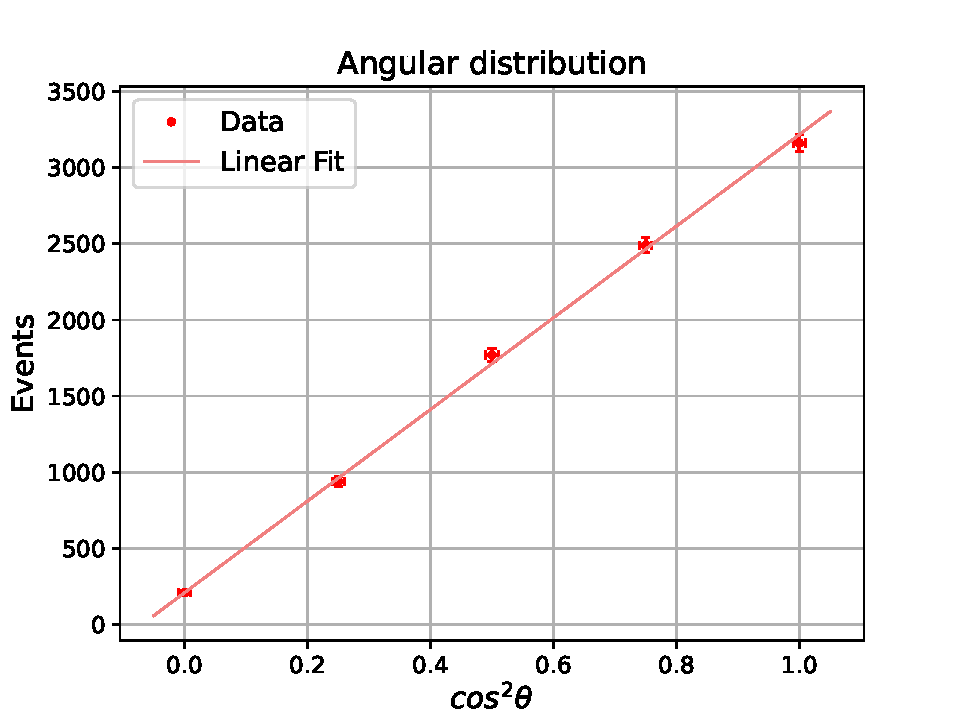
\includegraphics[width=0.48\linewidth]{linear_graph/ang_distr.pdf}
    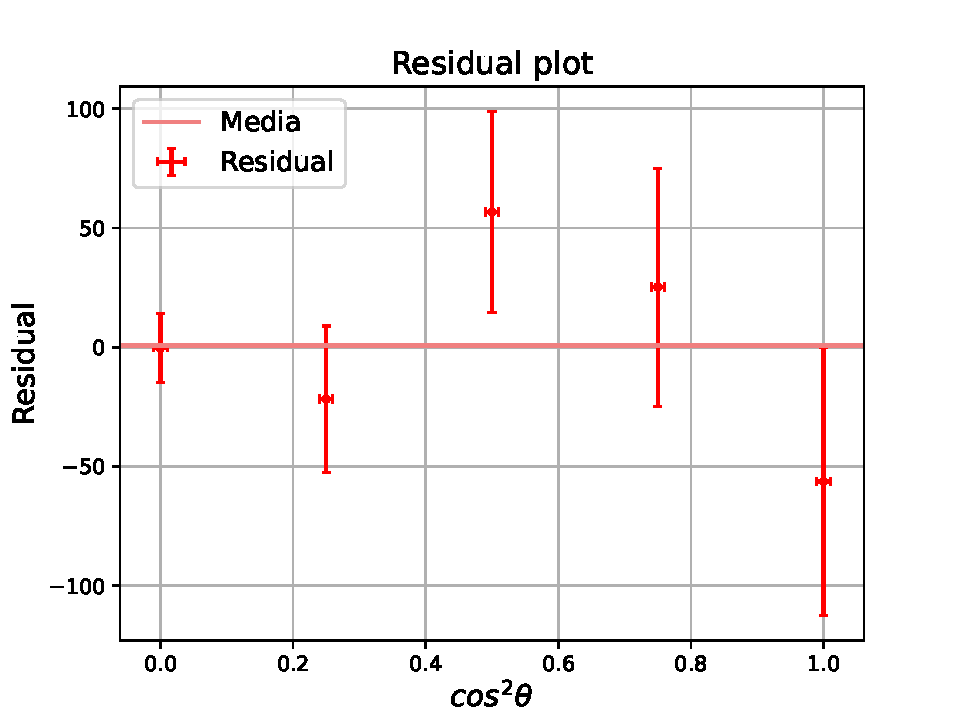
\includegraphics[width=0.48\linewidth]{linear_graph/res_ang_distr.pdf}
    \caption{Linear dependence on $\mathrm{cos}^2\theta$ of the number of particles detected by the telescope in a 15 minutes long acquisition (see Tab. \ref{tab:cos^2})}
    \label{fig: cos^2}
\end{figure}

\section{Results and conclusions}\label{sect:conclusions}
Hereafter an overview of the main results of this experiment.

The preliminary analysis of the signals and the creation of the coincidences have been successfully done. After the calibration of the three TACs, the outputs of the TACs, together with the logic signals from the trackers coincidence, were recorded overnight for $\mathtt{UP\wedge DOWN}$ events.

Apart from a narrow depletion in the middle and a possible inaccuracy in the intercept of TAC UP calibration, the 16-seconds-wide shapes of the calibrated time spectra are in agreement with the expectations. The calibration in position, which exploits the T coincidence, is compatible with the expected results. Furthermore, as a further validation of the analysis in both time and position, the time difference between the centroids in positions spectra is in line with the expected value derived considering the speed of the scintillation light inside the scintillators.

Correlations between the impact positions of muons on upper and lower scintillators have led to results in qualitative agreement with the expected ones, i.e. a positive correlation between position UP and position DOWN, a peaked distribution of $x_\mathrm{D}$ as $x_\mathrm{U}$ is fixed and a DOWN-UP time difference decreasing with $x_\mathrm{D}$.

The measured efficiency of the telescope with respect to the trackers is $r=(14\pm6)\%$. Since an accurate estimate of the geometrical acceptance has not been calculated, the contribution of the detection efficiency has not been evaluated.

The study of the angular distribution of cosmic rays with respect to the zenith was performed considering only a statistical error on the number of recorded events, assumed to be Poisson distributed. The angular distribution shows a good linearity in $\cos^2\theta$, even though the proportionality relation is not perfectly satisfied because of the finite width of the telescope.
% \begin{itemize}
%     \item[-] The preliminary analysis of the signals and the built up of the coincidences has been successfully done as shown by picture of the signals on the oscilloscope and by the calculation of the event rate made with the CAEN scaler. Furthermore the following analysis was coherent with the expectations.
%     \item[-] The calibration of the TAC in time shows that
%     %tac up time spostata
%     %tac up - down da commentare
%     %buco in mezzo
%     ; instead the calibration in position, which exploits the coincidence built at the beginning, was compatible with the expected result. Furthermore, as another validation of the analysis in both time and position, the time difference between the centroids in positions spectra is compatible with the expected value derived considering the speed of the scintillation light on the scintillators.
%     \item[-] Correlations between the impact positions of muons on upper and lower scintillators have been deeply studied on the devoted section, with results in agreement with the expected results.
%     \item[-] Efficiency
%     \item[-] The study of the angular distribution of cosmic rays respect to the zenith shows a good linearity that confirms the function $f(\theta)=k\cdot cos^2\theta$.
% \end{itemize}

\end{document}

